%%%%%%%%%%%%%%%%%%%%%%%%%%%%%%%%%%%%%%%%%%%%%%%%%%%%%%%%%%%%%%%%%%%%%%%%%%%
%% This file is part of the book
%%
%% Algorithmic Graph Theory
%% http://code.google.com/p/graph-theory-algorithms-book/
%%
%% Copyright (C) 2010 David Joyner <wdjoyner@gmail.com>
%% Copyright (C) 2009, 2010, 2011 Minh Van Nguyen <nguyenminh2@gmail.com>
%%
%% See the file COPYING for copying conditions.
%%%%%%%%%%%%%%%%%%%%%%%%%%%%%%%%%%%%%%%%%%%%%%%%%%%%%%%%%%%%%%%%%%%%%%%%%%%

\chapter{Tree Data Structures}
\label{chap:tree_data_structures}

\begin{quote}
\footnotesize
\includegraphics[scale=0.7]{image/tree-data-structures/tree.png} \\
\noindent
--- Randall Munroe\index{Munroe, Randall}, xkcd,
\url{http://xkcd.com/835/}
\end{quote}

\noindent
In Chapters~\ref{chap:graph_algorithms} and~\ref{chap:trees_forests},
we discussed various algorithms that rely on
priority\index{priority queue} queues as one of their fundamental data
structures. Such algorithms include
Dijkstra's\index{Dijkstra!algorithm} algorithm,
Prim's\index{Prim!algorithm} algorithm, and the algorithm for
constructing Huffman\index{Huffman tree} trees. The runtime of any
algorithm that uses priority queues crucially depends on an efficient
implementation of the priority queue data\index{data structure}
structure. This chapter discusses the general priority queue data
structure and various efficient implementations based on trees.
Section~\ref{sec:tree_data_structures:priority_queues} provides some
theoretical underpinning of priority queues and considers a simple
implementation of priority queues as sorted lists.
Section~\ref{sec:tree_data_structures:binary_heaps} discusses how to
use binary\index{binary tree} trees to realize an efficient
implementation of priority queues called a binary\index{binary heap}
heap. Although very useful in practice, binary heaps do not lend
themselves to being merged in an efficient manner, a setback rectified
in section~\ref{sec:tree_data_structures:binomial_heaps} by a priority
queue implementation called binomial\index{binomial heap} heaps. As a
further application of binary\index{binary tree} trees,
section~\ref{sec:tree_data_structures:binary_search_trees} discusses
binary\index{binary search tree} search trees as a general data
structure for managing data in a sorted order.


%%%%%%%%%%%%%%%%%%%%%%%%%%%%%%%%%%%%%%%%%%%%%%%%%%%%%%%%%%%%%%%%%%%%%%%%%%%

\section{Priority queues}
\label{sec:tree_data_structures:priority_queues}

A \emph{priority queue}\index{priority queue} is essentially a queue
data structure with various accompanying rules regarding how to access
and manage elements of the queue. Recall from
section~\ref{subsec:graph_algorithms:breadth_first_search} that an
ordinary queue $Q$ has the following basic accompanying functions for
assessing and managing its elements:
%%
\begin{itemize}
\item $\dequeue(Q)$ --- Remove the front of $Q$.

\item $\enqueue(Q, e)$ --- Append the element $e$ to the end of $Q$.
\end{itemize}

If $Q$ is now a priority queue, each element is associated with a key
or priority $p \in X$ from a totally ordered\index{total order} set
$X$. A binary relation denoted by an infix operator, say ``$\leq$'',
is defined on all elements of $X$ such that the following properties
hold for all $a,b,c \in X$:
%%
\begin{itemize}
\item Totality: We have $a \leq b$ or $b \leq a$.

\item Antisymmetry: If $a \leq b$ and $b \leq a$, then $a = b$.

\item Transitivity: If $a \leq b$ and $b \leq c$, then $a \leq c$.
\end{itemize}
%%
If the above three properties hold for the relation ``$\leq$'', then we
say that ``$\leq$'' is a \emph{total order}\index{total order} on $X$
and that $X$ is a
\emph{totally ordered set}\index{set!totally ordered}. In all, if the
key of each element of $Q$ belongs to the same totally ordered
set $X$, we use the total order defined on $X$ to compare the keys of
the queue elements. For example, the set $\Z$ of integers is totally
ordered by the ``less than or equal to'' relation. If the key of each
$e \in Q$ is an element of $\Z$, we use the latter relation to compare
the keys of elements of $Q$. In the case of an ordinary queue, the
key of each queue element is its position index.

To extract from a priority\index{priority queue} queue $Q$ an element
of lowest priority, we need to define the notion of smallest
priority or key. Let $p_i$ be the priority or key assigned to element
$e_i$ of $Q$. Then $p_{\min}$ is the lowest key if $p_{\min} \leq p$
for any element key $p$. The element with corresponding key
$p_{\min}$ is the minimum priority element. Based upon the notion of
key comparison, we define two operations on a priority queue:
%%
\begin{itemize}
\item $\insertElem(Q, e, p)$ --- Insert into $Q$ the element $e$ with
  key $p$.

\item $\extractMin(Q)$ --- Extract from $Q$ an element having the
  smallest priority.
\end{itemize}

An immediate application of priority queues is sorting a finite
sequence of items. Suppose $L$ is a finite list of $n > 0$ items on
which a total order is defined. Let $Q$ be an empty priority queue. In
the first phase of the priority queue sorting algorithm, we extract
each element $e \in L$ from $L$ and insert $e$ into $Q$ with key $e$
itself. In other words, each element $e$ is its own key. This first
phase of the sorting algorithm requires $n$ element extractions from
$L$ and $n$ element insertions into $Q$. The second phase of the
algorithm involves extracting elements from $Q$ via the $\extractMin$
operation. Queue elements are extracted via $\extractMin$ and inserted
back into $L$ in the order in which they are extracted from
$Q$. Algorithm~\ref{alg:tree_data_structures:priority_queue_sort}
presents pseudocode of our discussion. The runtime of
Algorithm~\ref{alg:tree_data_structures:priority_queue_sort} depends
on how the priority queue $Q$ is implemented.

\begin{algorithm}[!htbp]
%%%%%%%%%%%%%%%%%%%%%%%%%%%%%%%%%%%%%%%%%%%%%%%%%%%%%%%%%%%%%%%%%%%%%%%%%%%
%% This file is part of the book
%%
%% Algorithmic Graph Theory
%% http://code.google.com/p/graph-theory-algorithms-book/
%%
%% Copyright (C) 2009, 2010 Minh Van Nguyen <nguyenminh2@gmail.com>
%%
%% See the file COPYING for copying conditions.
%%%%%%%%%%%%%%%%%%%%%%%%%%%%%%%%%%%%%%%%%%%%%%%%%%%%%%%%%%%%%%%%%%%%%%%%%%%

\DontPrintSemicolon
\SetAlgoNoLine
%%
%% data section
\SetKwInOut{Input}{Input}
\SetKwInOut{Output}{Output}
%%
%% input/output
\Input{A finite list $L$ of $n > 0$ elements on which a total order is
  defined.}
\Output{The same list $L$ sorted by the total order relation defined
  on its elements.}
\BlankLine
%%
%% algorithm body
$Q \assign [\,]$\;
\For{$i \assign 1, 2, \dots, n$}{
  $e \assign \dequeue(L)$\;
  $\insertElem(Q, e, e)$\;
}
\For{$i \assign 1, 2, \dots, n$}{
  $e \assign \extractMin(Q)$\;
  $\enqueue(L, e)$\;
}

\caption{Sorting a sequence via priority queue.}
\label{alg:tree_data_structures:priority_queue_sort}
\end{algorithm}


%%%%%%%%%%%%%%%%%%%%%%%%%%%%%%%%%%%%%%%%%%%%%%%%%%%%%%%%%%%%%%%%%%%%%%%%%%%

\subsection{Sequence implementation}
\label{subsec:tree_data_structures:sequence_implementation}

A simple way to implement a priority queue is to maintain a sorted
sequence. Let $e_0, e_1, \dots, e_n$ be a sequence of $n + 1$ elements
with corresponding keys $\kappa_0, \kappa_1, \dots, \kappa_n$ and
suppose that the $\kappa_i$ all belong to the same totally ordered set
$X$ having total order $\leq$. Using the total order, we assume that
the $\kappa_i$ are sorted as
\[
\kappa_0 \leq \kappa_1 \leq \cdots \leq \kappa_n
\]
and $e_i \leq e_j$ if and only if $\kappa_i \leq \kappa_j$. Then we
consider the queue $Q = [e_0, e_1, \dots, e_n]$ as a priority queue in
which the head is always the minimum element and the tail is always
the maximum element. Extracting the minimum element is simply a
dequeue operation that can be accomplished in constant time
$O(1)$. However, inserting a new element into $Q$ takes linear time.

Let $e$ be an element with corresponding key $\kappa \in X$. Inserting
$e$ into $Q$ requires that we maintain elements of $Q$ sorted
according to the total order $\leq$. If $Q$ is empty, we simply
enqueue $e$ into $Q$. Suppose now that $Q$ is a nonempty priority
queue. If $\kappa \leq \kappa_0$, then $e$ becomes the new head of
$Q$. If $\kappa_n \leq \kappa$, then $e$ becomes the new tail of
$Q$. Inserting a new head or tail into $Q$ each requires constant time
$O(1)$. However, if $\kappa_1 \leq \kappa \leq \kappa_{n-1}$ then we
need to traverse $Q$ starting from $e_1$, searching for a position at
which to insert $e$. Let $e_i$ be the queue element at position $i$
within $Q$. If $\kappa \leq \kappa_i$ then we insert $e$ into $Q$ at
position $i$, thus moving $e_i$ to position $i + 1$. Otherwise we next
consider $e_{i+1}$ and repeat the above comparison process. By
hypothesis, $\kappa_1 \leq \kappa \leq \kappa_{n-1}$ and therefore
inserting $e$ into $Q$ takes a worst-case runtime of $O(n)$.


%%%%%%%%%%%%%%%%%%%%%%%%%%%%%%%%%%%%%%%%%%%%%%%%%%%%%%%%%%%%%%%%%%%%%%%%%%%

\section{Binary heaps}
\label{sec:tree_data_structures:binary_heaps}
\index{binary heap}

A sequence implementation of priority queues has the advantage of
being simple to understand. Inserting an element into a sequence-based
priority queue requires linear time, which can quickly become
infeasible for queues containing hundreds of thousands or even
millions of elements. Can we do any better? Rather than using a sorted
sequence, we can use a binary tree to realize an implementation of
priority queues that is much more efficient than a sequence-based
implementation. In particular, we use a data structure called a
\emph{binary heap}\index{binary heap}, which allows for element
insertion in logarithmic time.

In~\cite{Williams1964}, Williams\index{Williams, J. W. J.} introduced
the heapsort\index{heapsort} algorithm and described how to implement
a priority queue using a binary\index{binary heap} heap. A basic idea
is to consider queue elements as internal vertices in a binary tree
$T$, with external vertices or leaves being ``place-holders''. The
tree $T$ satisfies two further properties:
%%
\begin{enumerate}
\item A relational property specifying the relative ordering and
  placement of queue elements.

\item A structural property that specifies the structure of $T$.
\end{enumerate}
%%
The relational property of $T$ can be expressed as follows:

\begin{definition}
\textbf{Heap-order property.}\index{binary heap!order property}
Let $T$ be a binary tree and let $v$ be a vertex of $T$ other than the
root. If $p$ is the parent of $v$ and these vertices have corresponding
keys $\kappa_p$ and $\kappa_v$, respectively, then
$\kappa_p \leq \kappa_v$.
\end{definition}

The heap-order property\index{binary heap!order property} is defined in terms
of the total order used to compare the keys of the internal
vertices. Taking the total order to be the ordinary
``less than or equal to'' relation, it follows from the heap-order
property that the root of $T$ is always the vertex with a minimum
key. Similarly, if the total order is the usual
``greater than or equal to'' relation, then the root of $T$ is always
the vertex with a maximum key. In general, if $\leq$ is a total order
defined on the keys of $T$ and $u$ and $v$ are vertices of $T$, we say
that $u$ is less than or equal to $v$ if and only if $u \leq v$.
Furthermore, $u$ is said to be a minimum vertex of $T$ if and only if
$u \leq v$ for all vertices of $T$. From our discussion above, the
root is always a minimum vertex of $T$ and is said to be ``at the top
of the heap'', from which we derive the name ``heap'' for this data
structure.

Another consequence of the heap-order\index{binary heap!order property}
property becomes apparent when we trace out a path from the root of
$T$ to any internal vertex. Let $r$ be the root of $T$ and let $v$ be
any internal vertex of $T$. If $r, v_0, v_1, \dots, v_n, v$ is an
$r$-$v$ path with corresponding keys
\[
\kappa_r, \kappa_{v_0}, \kappa_{v_1}, \dots, \kappa_{v_n}, \kappa_v
\]
then we have
\[
\kappa_r \leq \kappa_{v_0} \leq \kappa_{v_1} \leq \cdots \leq
\kappa_{v_n} \leq \kappa_v.
\]
In other words, the keys encountered on the path from $r$ to $v$ are
arranged in nondecreasing order.

The structural property of $T$ is used to enforce that $T$ be of as
small a height as possible. Before stating the structural property, we
first define the level\index{level!binary tree} of a binary
tree. Recall that the depth of a vertex in $T$ is its distance from
the root. Level\index{level!binary tree} $i$ of a binary tree $T$
refers to all vertices of $T$ that have the same depth $i$. We are now
ready to state the heap-structure property.

\begin{definition}
\textbf{Heap-structure property.}\index{binary heap!structure property}
Let $T$ be a binary tree with height $h$. Then $T$ satisfies the
heap-structure property if $T$ is nearly a
complete\index{binary tree!nearly complete} binary tree. That is, level
$0 \leq i \leq h - 1$ has $2^i$ vertices, whereas level $h$ has
$\leq 2^h$ vertices. The vertices at level $h$ are filled from left to
right.
\end{definition}

\begin{figure}[!htbp]
\centering
%%%%%%%%%%%%%%%%%%%%%%%%%%%%%%%%%%%%%%%%%%%%%%%%%%%%%%%%%%%%%%%%%%%%%%%%%%%
%% This file is part of the book
%%
%% Algorithmic Graph Theory
%% http://code.google.com/p/graph-theory-algorithms-book/
%%
%% Copyright (C) 2009, 2010, 2011 Minh Van Nguyen <nguyenminh2@gmail.com>
%%
%% See the file COPYING for copying conditions.
%%%%%%%%%%%%%%%%%%%%%%%%%%%%%%%%%%%%%%%%%%%%%%%%%%%%%%%%%%%%%%%%%%%%%%%%%%%

\documentclass{article}

\usepackage{subfigure}
\usepackage{tikz}
\usetikzlibrary{external}
\usetikzlibrary{trees}
\tikzexternalize{sample-binary-heaps}

\begin{document}

\begin{figure}
\subfigure[]{
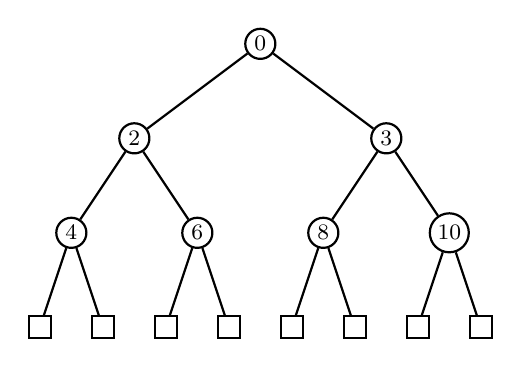
\begin{tikzpicture}
[-,thick,%
  every node/.style={shape=circle,inner sep=1.5pt,draw,thick},%
  scale=0.8]
\footnotesize
\node {$0$}
  [sibling distance=4cm]
  child {node {$2$}
    [sibling distance=2cm]
    child {node {$4$}
      [sibling distance=1cm]
      child {node[rectangle,inner sep=4pt,draw,thick] {}}
      child {node[rectangle,inner sep=4pt,draw,thick] {}}
    }
    child {node {$6$}
      [sibling distance=1cm]
      child {node[rectangle,inner sep=4pt,draw,thick] {}}
      child {node[rectangle,inner sep=4pt,draw,thick] {}}
    }
  }
  child {node {$3$}
    [sibling distance=2cm]
    child {node {$8$}
      [sibling distance=1cm]
      child {node[rectangle,inner sep=4pt,draw,thick] {}}
      child {node[rectangle,inner sep=4pt,draw,thick] {}}
    }
    child {node {$10$}
      [sibling distance=1cm]
      child {node[rectangle,inner sep=4pt,draw,thick] {}}
      child {node[rectangle,inner sep=4pt,draw,thick] {}}
    }
  };
\end{tikzpicture}
}
%%
%%
\subfigure[]{
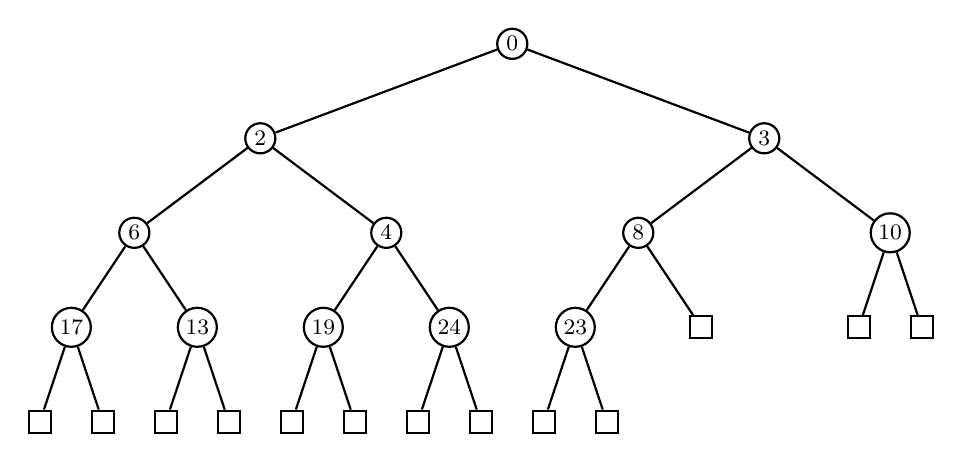
\begin{tikzpicture}
[-,thick,%
  every node/.style={shape=circle,inner sep=1.5pt,draw,thick},%
  scale=0.8]
\footnotesize
\node {$0$}
  [sibling distance=8cm]
  child {node {$2$}
    [sibling distance=4cm]
    child {node {$6$}
      [sibling distance=2cm]
      child {node {$17$}
        [sibling distance=1cm]
        child {node[rectangle,inner sep=4pt,draw,thick] {}}
        child {node[rectangle,inner sep=4pt,draw,thick] {}}
      }
      child {node {$13$}
        [sibling distance=1cm]
        child {node[rectangle,inner sep=4pt,draw,thick] {}}
        child {node[rectangle,inner sep=4pt,draw,thick] {}}
      }
    }
    child {node {$4$}
      [sibling distance=2cm]
      child {node {$19$}
        [sibling distance=1cm]
        child {node[rectangle,inner sep=4pt,draw,thick] {}}
        child {node[rectangle,inner sep=4pt,draw,thick] {}}
      }
      child {node {$24$}
        [sibling distance=1cm]
        child {node[rectangle,inner sep=4pt,draw,thick] {}}
        child {node[rectangle,inner sep=4pt,draw,thick] {}}
      }
    }
  }
  child {node {$3$}
    [sibling distance=4cm]
    child {node {$8$}
      [sibling distance=2cm]
      child {node {$23$}
        [sibling distance=1cm]
        child {node[rectangle,inner sep=4pt,draw,thick] {}}
        child {node[rectangle,inner sep=4pt,draw,thick] {}}
      }
      child {node[rectangle,inner sep=4pt,draw,thick] {}}
    }
    child {node {$10$}
      [sibling distance=1cm]
      child {node[rectangle,inner sep=4pt,draw,thick] {}}
      child {node[rectangle,inner sep=4pt,draw,thick] {}}
    }
  };
\end{tikzpicture}
}
%%
%%
\subfigure[]{
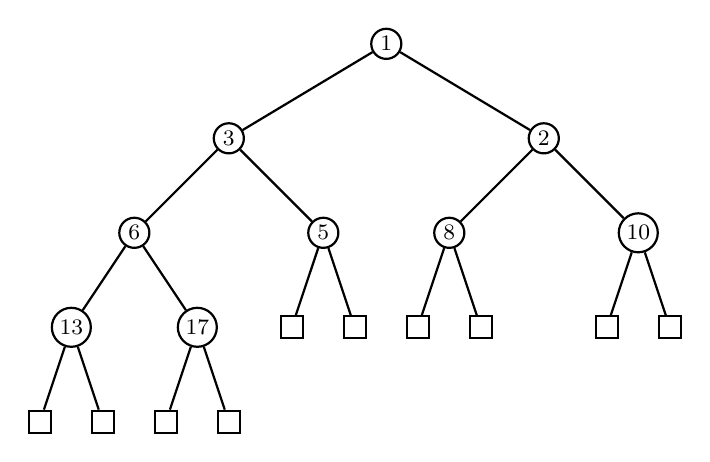
\begin{tikzpicture}
[-,thick,%
  every node/.style={shape=circle,inner sep=1.5pt,draw,thick},%
  scale=0.8]
\footnotesize
\node {$1$}
  [sibling distance=5cm]
  child {node {$3$}
    [sibling distance=3cm]
    child {node {$6$}
      [sibling distance=2cm]
      child {node {$13$}
        [sibling distance=1cm]
        child {node[rectangle,inner sep=4pt,draw,thick] {}}
        child {node[rectangle,inner sep=4pt,draw,thick] {}}
      }
      child {node {$17$}
        [sibling distance=1cm]
        child {node[rectangle,inner sep=4pt,draw,thick] {}}
        child {node[rectangle,inner sep=4pt,draw,thick] {}}
      }
    }
    child {node {$5$}
      [sibling distance=1cm]
      child {node[rectangle,inner sep=4pt,draw,thick] {}}
      child {node[rectangle,inner sep=4pt,draw,thick] {}}
    }
  }
  child {node {$2$}
    [sibling distance=3cm]
    child {node {$8$}
      [sibling distance=1cm]
      child {node[rectangle,inner sep=4pt,draw,thick] {}}
      child {node[rectangle,inner sep=4pt,draw,thick] {}}
    }
    child {node {$10$}
      [sibling distance=1cm]
      child {node[rectangle,inner sep=4pt,draw,thick] {}}
      child {node[rectangle,inner sep=4pt,draw,thick] {}}
    }
  };
\end{tikzpicture}
}
\end{figure}

\end{document}

\caption{Examples of binary heaps with integer keys.}
\label{fig:tree_data_structures:binary_heaps_integer_keys}
\end{figure}

If a binary tree $T$ satisfies both the heap-order and heap-structure
properties, then $T$ is referred to as a binary heap. By insisting
that $T$ satisfy the heap-order\index{binary heap!order property} property,
we are able to determine the minimum vertex of $T$ in constant time
$O(1)$. Requiring that $T$ also satisfy the
heap-structure\index{binary heap!structure property} property allows us to
determine the last vertex of $T$. The last vertex of $T$ is identified
as the right-most internal vertex of $T$ having the greatest depth.
Figure~\ref{fig:tree_data_structures:binary_heaps_integer_keys}
illustrates various examples of binary heaps. The heap-structure
property together with
Theorem~\ref{thm:trees_forests:complete_binary_tree_exact_order}
result in the following corollary on the height of a binary heap.

\begin{corollary}
\label{cor:tree_data_structures:height_binary_heap}
A binary heap $T$ with $n$ internal vertices has height
\[
h
=
\big\lceil \lg(n + 1) \big\rceil.\index{$\lg$}
\]
\end{corollary}

\begin{proof}
Level $h - 1$ has at least one internal vertex. Apply
Theorem~\ref{thm:trees_forests:complete_binary_tree_exact_order} to
see that $T$ has at least
\[
2^{h - 2 + 1} - 1 + 1
=
2^{h - 1}
\]
internal vertices. On the other hand, level $h - 1$ has at most
$2^{h-1}$ internal vertices. Another application of
Theorem~\ref{thm:trees_forests:complete_binary_tree_exact_order} shows
that $T$ has at most
\[
2^{h - 1 + 1} - 1
=
2^h - 1
\]
internal vertices. Thus $n$ is bounded by
\[
2^{h - 1} \leq n \leq 2^h - 1.
\]
Taking logarithms of each side in the latter bound results in
\[
\lg(n + 1) \leq h \leq \lg n + 1
\]
and the corollary follows.
\end{proof}

\begin{figure}[!htbp]
\centering
%%%%%%%%%%%%%%%%%%%%%%%%%%%%%%%%%%%%%%%%%%%%%%%%%%%%%%%%%%%%%%%%%%%%%%%%%%%
%% This file is part of the book
%%
%% Algorithmic Graph Theory
%% http://code.google.com/p/graph-theory-algorithms-book/
%%
%% Copyright (C) 2009, 2010, 2011 Minh Van Nguyen <nguyenminh2@gmail.com>
%%
%% See the file COPYING for copying conditions.
%%%%%%%%%%%%%%%%%%%%%%%%%%%%%%%%%%%%%%%%%%%%%%%%%%%%%%%%%%%%%%%%%%%%%%%%%%%

\documentclass{article}

\usepackage{subfigure}
\usepackage{tikz}
\usetikzlibrary{external}
\tikzexternalize{sample-binary-heaps-array}

\begin{document}

\begin{figure}
\subfigure[]{
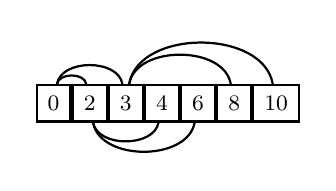
\begin{tikzpicture}
[every node/.style={inner sep=4pt,draw,thick},%
  lineDecorate/.style={-,thick}]
\footnotesize
\pgfmatrix{rectangle}{center}{}
{\pgfusepath{}}{\pgfpointorigin}{\let\&=\pgfmatrixnextcell}
{
  \node(0){$0$}; \& \node(2){$2$}; \& \node(3){$3$}; \& \node(4){$4$}; \&
  \node(6){$6$}; \& \node(8){$8$}; \& \node(10){$10$}; \\
}
\path
\foreach \startNode/\endNode/\bend in {
  0/2/bend left, 0/3/bend left, 2/4/bend right, 2/6/bend right,
  3/8/bend left, 3/10/bend left}
{
  (\startNode) edge[lineDecorate,\bend=80] (\endNode)
};
\end{tikzpicture}
}
%%
%%
\qquad
\subfigure[]{
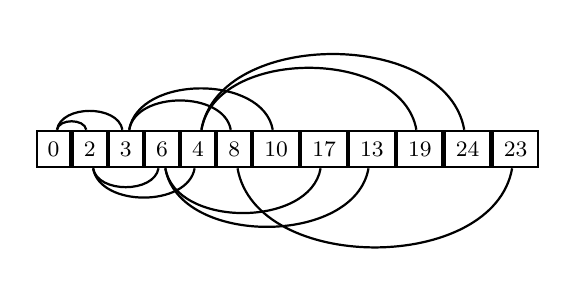
\begin{tikzpicture}
[every node/.style={inner sep=4pt,draw,thick},%
  lineDecorate/.style={-,thick}]
\footnotesize
\pgfmatrix{rectangle}{center}{}
{\pgfusepath{}}{\pgfpointorigin}{\let\&=\pgfmatrixnextcell}
{
  \node(0){$0$}; \& \node(2){$2$}; \& \node(3){$3$}; \& \node(6){$6$}; \&
  \node(4){$4$}; \& \node(8){$8$}; \& \node(10){$10$}; \& \node(17){$17$}; \&
  \node(13){$13$}; \& \node(19){$19$}; \& \node(24){$24$}; \&
  \node(23){$23$}; \\
}
\path
\foreach \startNode/\endNode/\bend in {
  0/2/bend left, 0/3/bend left, 2/6/bend right, 2/4/bend right,
  3/8/bend left, 3/10/bend left, 6/17/bend right, 6/13/bend right,
  4/19/bend left, 4/24/bend left, 8/23/bend right}
{
  (\startNode) edge[lineDecorate,\bend=80] (\endNode)
};
\end{tikzpicture}
}
%%
%%
\subfigure[]{
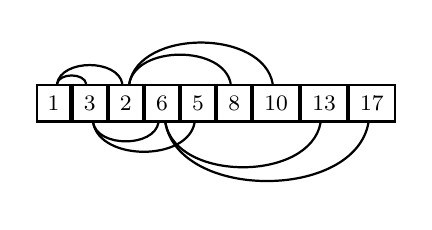
\begin{tikzpicture}
[every node/.style={inner sep=4pt,draw,thick},%
  lineDecorate/.style={-,thick}]
\footnotesize
\pgfmatrix{rectangle}{center}{}
{\pgfusepath{}}{\pgfpointorigin}{\let\&=\pgfmatrixnextcell}
{
  \node(1){$1$}; \& \node(3){$3$}; \& \node(2){$2$}; \& \node(6){$6$}; \&
  \node(5){$5$}; \& \node(8){$8$}; \& \node(10){$10$}; \&
  \node(13){$13$}; \& \node(17){$17$}; \\
}
\path
\foreach \startNode/\endNode/\bend in {
  1/3/bend left, 1/2/bend left, 3/6/bend right, 3/5/bend right,
  2/8/bend left, 2/10/bend left, 6/13/bend right, 6/17/bend right}
{
  (\startNode) edge[lineDecorate,\bend=80] (\endNode)
};
\end{tikzpicture}
}
\end{figure}

\end{document}

\caption{Sequence representations of various binary heaps.}
\label{fig:tree_data_structures:sequence_representations_binary_heaps}
\end{figure}


%%%%%%%%%%%%%%%%%%%%%%%%%%%%%%%%%%%%%%%%%%%%%%%%%%%%%%%%%%%%%%%%%%%%%%%%%%%

\subsection{Sequence representation}

Any binary heap can be represented as a binary tree. Each vertex in
the tree must know about its parent and its two children. However, a
more common approach is to represent a binary heap as a sequence such
as a list, array, or vector. Let $T$ be a binary heap consisting of
$n$ internal vertices and let $L$ be a list of $n$ elements. The root
vertex is represented as the list element $L[0]$. For each index $i$,
the children of $L[i]$ are $L[2i + 1]$ and $L[2i + 2]$ and the parent
of $L[i]$ is
\[
L\left[ \left\lfloor \frac{i - 1}{2} \right\rfloor \right].
\]
With a sequence representation of a binary heap, each vertex needs not
know about its parent and children. Such information can be obtained
via simple arithmetic on sequence indices. For example, the binary
heaps in
Figure~\ref{fig:tree_data_structures:binary_heaps_integer_keys} can be
represented as the corresponding lists in
Figure~\ref{fig:tree_data_structures:sequence_representations_binary_heaps}.
Note that it is not necessary to store the leaves of $T$ in the
sequence representation.


%%%%%%%%%%%%%%%%%%%%%%%%%%%%%%%%%%%%%%%%%%%%%%%%%%%%%%%%%%%%%%%%%%%%%%%%%%%

\subsection{Insertion and sift-up}
\label{subsec:tree_data_structures:insertion_sift_up}

We now consider the problem of inserting a vertex $v$ into a binary
heap $T$. If $T$ is empty, inserting a vertex simply involves the
creation of a new internal vertex. We let that new internal vertex be
$v$ and let its two children be leaves. The resulting binary heap
augmented with $v$ has exactly one internal vertex and satisfies both
the heap-order and heap-structure properties, as shown in
Figure~\ref{fig:tree_data_structures:insert_vertex_into_empty_binary_heap}.
In other words, any binary heap with one internal vertex trivially
satisfies the heap-order property.

\begin{figure}[!htbp]
\centering
\input{image/tree-data-structures/binary-heap-insert-empty.tex}
\caption{Inserting a vertex into an empty binary heap.}
\label{fig:tree_data_structures:insert_vertex_into_empty_binary_heap}
\end{figure}

Let $T$ now be a nonempty binary heap, i.e. $T$ has at least one
internal vertex, and suppose we want to insert into $T$ an internal
vertex $v$. We must identify the correct leaf of $T$ at which to
insert $v$. If the $n$ internal vertices of $T$ are
$r = v_0, v_1, \dots, v_{n-1}$, then by the sequence representation of
$T$ we can identify the last internal vertex $v_{n-1}$ in constant
time. The correct leaf at which to insert $v$ is the sequence element
immediately following $v_{n-1}$, i.e. the element at position $n$ in
the sequence representation of $T$. We replace with $v$ the leaf at
position $n$ in the sequence so that $v$ now becomes the last vertex
of $T$.

The binary heap $T$ augmented with the new last vertex $v$ satisfies
the heap-structure property, but may violate the heap-order
property. To ensure that $T$ satisfies the heap-order property, we
perform an operation on $T$ called
\emph{sift-up}\index{binary heap!sift-up} that involves possibly
moving $v$ up through various levels of $T$. Let $\kappa_v$ be the key
of $v$ and let $\kappa_{p(v)}$ be the key of $v$'s parent. If the
relation $\kappa_{p(v)} \leq \kappa_v$ holds, then $T$ satisfies the
heap-order property. Otherwise we swap $v$ with its parent,
effectively moving $v$ up one level to be at the position previously
occupied by its parent. The parent of $v$ is moved down one level and
now occupies the position where $v$ was previously. With $v$ in its
new position, we perform the same key comparison process with $v$'s
new parent. The key comparison and swapping continue until the
heap-order property holds for $T$. In the worst case, $v$ would become
the new root of $T$ after undergoing a number of swaps that is
proportional to the height of $T$. Therefore, inserting a new internal
vertex into $T$ can be achieved in time $O(\lg n)$.
Figure~\ref{fig:tree_data_structures:insert_sift_up_binary_heap}
illustrates the insertion of a new internal vertex into a nonempty
binary heap and the resulting sift-up operation to maintain the
heap-order property.
Algorithm~\ref{alg:tree_data_structures:binary_heap_insert} presents
pseudocode of our discussion for inserting a new internal vertex into
a nonempty binary heap. The pseudocode is adapted from
Howard~\cite{Howard2010}, which provides a C implementation of binary
heaps.

\begin{figure}[!htbp]
\centering
%%%%%%%%%%%%%%%%%%%%%%%%%%%%%%%%%%%%%%%%%%%%%%%%%%%%%%%%%%%%%%%%%%%%%%%%%%%
%% This file is part of the book
%%
%% Algorithmic Graph Theory
%% http://code.google.com/p/graph-theory-algorithms-book/
%%
%% Copyright (C) 2009, 2010 Minh Van Nguyen <nguyenminh2@gmail.com>
%%
%% See the file COPYING for copying conditions.
%%%%%%%%%%%%%%%%%%%%%%%%%%%%%%%%%%%%%%%%%%%%%%%%%%%%%%%%%%%%%%%%%%%%%%%%%%%

\subfigure[]{
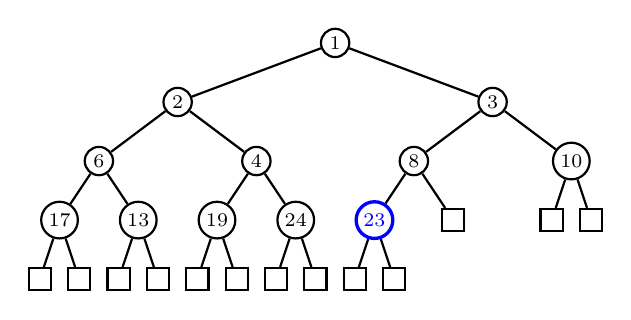
\begin{tikzpicture}
[-,thick,%
  every node/.style={shape=circle,inner sep=1.5pt,draw,thick},%
  scale=0.5]
\scriptsize
\node {$1$}
  [sibling distance=8cm]
  child {node {$2$}
    [sibling distance=4cm]
    child {node {$6$}
      [sibling distance=2cm]
      child {node {$17$}
        [sibling distance=1cm]
        child {node[rectangle,inner sep=4pt,draw,thick] {}}
        child {node[rectangle,inner sep=4pt,draw,thick] {}}
      }
      child {node {$13$}
        [sibling distance=1cm]
        child {node[rectangle,inner sep=4pt,draw,thick] {}}
        child {node[rectangle,inner sep=4pt,draw,thick] {}}
      }
    }
    child {node {$4$}
      [sibling distance=2cm]
      child {node {$19$}
        [sibling distance=1cm]
        child {node[rectangle,inner sep=4pt,draw,thick] {}}
        child {node[rectangle,inner sep=4pt,draw,thick] {}}
      }
      child {node {$24$}
        [sibling distance=1cm]
        child {node[rectangle,inner sep=4pt,draw,thick] {}}
        child {node[rectangle,inner sep=4pt,draw,thick] {}}
      }
    }
  }
  child {node {$3$}
    [sibling distance=4cm]
    child {node {$8$}
      [sibling distance=2cm]
      child {node[blue,very thick] {$23$}
        [sibling distance=1cm]
        child {node[rectangle,inner sep=4pt,draw,thick] {}}
        child {node[rectangle,inner sep=4pt,draw,thick] {}}
      }
      child {node[rectangle,inner sep=4pt,draw,thick] {}}
    }
    child {node {$10$}
      [sibling distance=1cm]
      child {node[rectangle,inner sep=4pt,draw,thick] {}}
      child {node[rectangle,inner sep=4pt,draw,thick] {}}
    }
  };
\end{tikzpicture}
}
%%
%%
\quad
\subfigure[]{
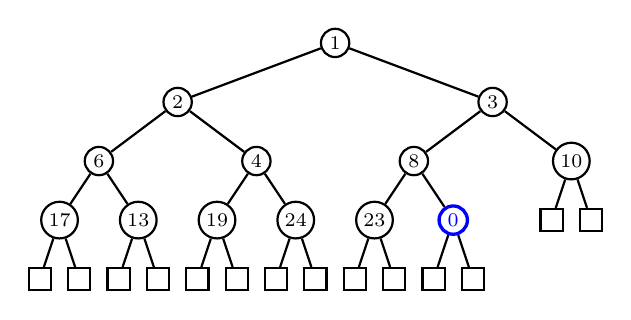
\begin{tikzpicture}
[-,thick,%
  every node/.style={shape=circle,inner sep=1.5pt,draw,thick},%
  scale=0.5]
\scriptsize
\node {$1$}
  [sibling distance=8cm]
  child {node {$2$}
    [sibling distance=4cm]
    child {node {$6$}
      [sibling distance=2cm]
      child {node {$17$}
        [sibling distance=1cm]
        child {node[rectangle,inner sep=4pt,draw,thick] {}}
        child {node[rectangle,inner sep=4pt,draw,thick] {}}
      }
      child {node {$13$}
        [sibling distance=1cm]
        child {node[rectangle,inner sep=4pt,draw,thick] {}}
        child {node[rectangle,inner sep=4pt,draw,thick] {}}
      }
    }
    child {node {$4$}
      [sibling distance=2cm]
      child {node {$19$}
        [sibling distance=1cm]
        child {node[rectangle,inner sep=4pt,draw,thick] {}}
        child {node[rectangle,inner sep=4pt,draw,thick] {}}
      }
      child {node {$24$}
        [sibling distance=1cm]
        child {node[rectangle,inner sep=4pt,draw,thick] {}}
        child {node[rectangle,inner sep=4pt,draw,thick] {}}
      }
    }
  }
  child {node {$3$}
    [sibling distance=4cm]
    child {node {$8$}
      [sibling distance=2cm]
      child {node {$23$}
        [sibling distance=1cm]
        child {node[rectangle,inner sep=4pt,draw,thick] {}}
        child {node[rectangle,inner sep=4pt,draw,thick] {}}
      }
      child {node[blue,very thick] {$0$}
        [sibling distance=1cm]
        child {node[rectangle,inner sep=4pt,draw,thick] {}}
        child {node[rectangle,inner sep=4pt,draw,thick] {}}
      }
    }
    child {node {$10$}
      [sibling distance=1cm]
      child {node[rectangle,inner sep=4pt,draw,thick] {}}
      child {node[rectangle,inner sep=4pt,draw,thick] {}}
    }
  };
\end{tikzpicture}
}
%%
%%
\subfigure[]{
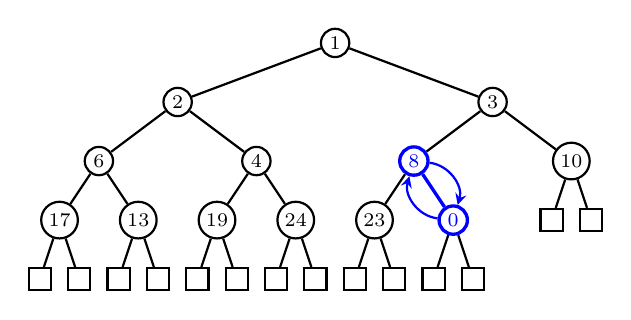
\begin{tikzpicture}
[-,thick,%
  every node/.style={shape=circle,inner sep=1.5pt,draw,thick},%
  scale=0.5]
\scriptsize
\node {$1$}
  [sibling distance=8cm]
  child {node {$2$}
    [sibling distance=4cm]
    child {node {$6$}
      [sibling distance=2cm]
      child {node {$17$}
        [sibling distance=1cm]
        child {node[rectangle,inner sep=4pt,draw,thick] {}}
        child {node[rectangle,inner sep=4pt,draw,thick] {}}
      }
      child {node {$13$}
        [sibling distance=1cm]
        child {node[rectangle,inner sep=4pt,draw,thick] {}}
        child {node[rectangle,inner sep=4pt,draw,thick] {}}
      }
    }
    child {node {$4$}
      [sibling distance=2cm]
      child {node {$19$}
        [sibling distance=1cm]
        child {node[rectangle,inner sep=4pt,draw,thick] {}}
        child {node[rectangle,inner sep=4pt,draw,thick] {}}
      }
      child {node {$24$}
        [sibling distance=1cm]
        child {node[rectangle,inner sep=4pt,draw,thick] {}}
        child {node[rectangle,inner sep=4pt,draw,thick] {}}
      }
    }
  }
  child {node {$3$}
    [sibling distance=4cm]
    child {node[blue,very thick] (8) {$8$}
      [sibling distance=2cm]
      child {node {$23$}
        [sibling distance=1cm]
        child {node[rectangle,inner sep=4pt,draw,thick] {}}
        child {node[rectangle,inner sep=4pt,draw,thick] {}}
      }
      child[blue,very thick] {node[blue,very thick] (0) {$0$}
        [sibling distance=1cm]
        child[black,thick] {node[rectangle,inner sep=4pt,draw,thick] {}}
        child[black,thick] {node[rectangle,inner sep=4pt,draw,thick] {}}
      }
    }
    child {node {$10$}
      [sibling distance=1cm]
      child {node[rectangle,inner sep=4pt,draw,thick] {}}
      child {node[rectangle,inner sep=4pt,draw,thick] {}}
    }
  };
\path
(0) edge[->,>=stealth,thick,bend left=50,blue] (8)
(8) edge[->,>=stealth,thick,bend left=50,blue] (0);
\end{tikzpicture}
}
%%
%%
\quad
\subfigure[]{
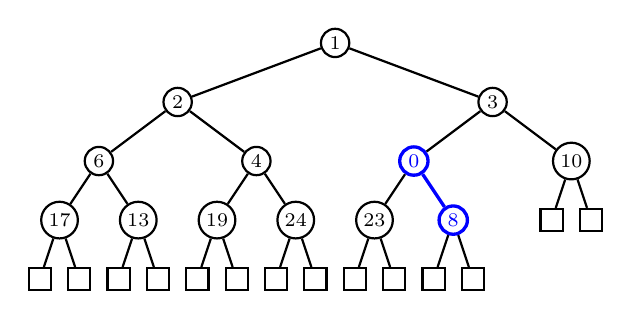
\begin{tikzpicture}
[-,thick,%
  every node/.style={shape=circle,inner sep=1.5pt,draw,thick},%
  scale=0.5]
\scriptsize
\node {$1$}
  [sibling distance=8cm]
  child {node {$2$}
    [sibling distance=4cm]
    child {node {$6$}
      [sibling distance=2cm]
      child {node {$17$}
        [sibling distance=1cm]
        child {node[rectangle,inner sep=4pt,draw,thick] {}}
        child {node[rectangle,inner sep=4pt,draw,thick] {}}
      }
      child {node {$13$}
        [sibling distance=1cm]
        child {node[rectangle,inner sep=4pt,draw,thick] {}}
        child {node[rectangle,inner sep=4pt,draw,thick] {}}
      }
    }
    child {node {$4$}
      [sibling distance=2cm]
      child {node {$19$}
        [sibling distance=1cm]
        child {node[rectangle,inner sep=4pt,draw,thick] {}}
        child {node[rectangle,inner sep=4pt,draw,thick] {}}
      }
      child {node {$24$}
        [sibling distance=1cm]
        child {node[rectangle,inner sep=4pt,draw,thick] {}}
        child {node[rectangle,inner sep=4pt,draw,thick] {}}
      }
    }
  }
  child {node {$3$}
    [sibling distance=4cm]
    child {node[blue,very thick] {$0$}
      [sibling distance=2cm]
      child {node {$23$}
        [sibling distance=1cm]
        child {node[rectangle,inner sep=4pt,draw,thick] {}}
        child {node[rectangle,inner sep=4pt,draw,thick] {}}
      }
      child[blue,very thick] {node[blue,very thick] {$8$}
        [sibling distance=1cm]
        child[black,thick] {node[rectangle,inner sep=4pt,draw,thick] {}}
        child[black,thick] {node[rectangle,inner sep=4pt,draw,thick] {}}
      }
    }
    child {node {$10$}
      [sibling distance=1cm]
      child {node[rectangle,inner sep=4pt,draw,thick] {}}
      child {node[rectangle,inner sep=4pt,draw,thick] {}}
    }
  };
\end{tikzpicture}
}
%%
%%
\subfigure[]{
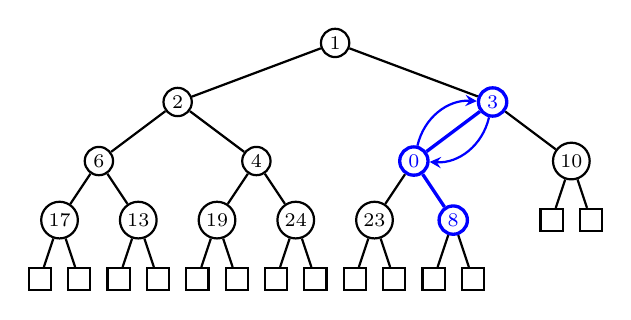
\begin{tikzpicture}
[-,thick,%
  every node/.style={shape=circle,inner sep=1.5pt,draw,thick},%
  scale=0.5]
\scriptsize
\node {$1$}
  [sibling distance=8cm]
  child {node {$2$}
    [sibling distance=4cm]
    child {node {$6$}
      [sibling distance=2cm]
      child {node {$17$}
        [sibling distance=1cm]
        child {node[rectangle,inner sep=4pt,draw,thick] {}}
        child {node[rectangle,inner sep=4pt,draw,thick] {}}
      }
      child {node {$13$}
        [sibling distance=1cm]
        child {node[rectangle,inner sep=4pt,draw,thick] {}}
        child {node[rectangle,inner sep=4pt,draw,thick] {}}
      }
    }
    child {node {$4$}
      [sibling distance=2cm]
      child {node {$19$}
        [sibling distance=1cm]
        child {node[rectangle,inner sep=4pt,draw,thick] {}}
        child {node[rectangle,inner sep=4pt,draw,thick] {}}
      }
      child {node {$24$}
        [sibling distance=1cm]
        child {node[rectangle,inner sep=4pt,draw,thick] {}}
        child {node[rectangle,inner sep=4pt,draw,thick] {}}
      }
    }
  }
  child {node[blue,very thick] (3) {$3$}
    [sibling distance=4cm]
    child[blue,very thick] {node[blue,very thick] (0) {$0$}
      [sibling distance=2cm]
      child[black,thick] {node {$23$}
        [sibling distance=1cm]
        child {node[rectangle,inner sep=4pt,draw,thick] {}}
        child {node[rectangle,inner sep=4pt,draw,thick] {}}
      }
      child[blue,very thick] {node[blue,very thick] {$8$}
        [sibling distance=1cm]
        child[black,thick] {node[rectangle,inner sep=4pt,draw,thick] {}}
        child[black,thick] {node[rectangle,inner sep=4pt,draw,thick] {}}
      }
    }
    child {node {$10$}
      [sibling distance=1cm]
      child {node[rectangle,inner sep=4pt,draw,thick] {}}
      child {node[rectangle,inner sep=4pt,draw,thick] {}}
    }
  };
\path
(0) edge[->,>=stealth,thick,bend left=40,blue] (3)
(3) edge[->,>=stealth,thick,bend left=40,blue] (0);
\end{tikzpicture}
}
%%
%%
\quad
\subfigure[]{
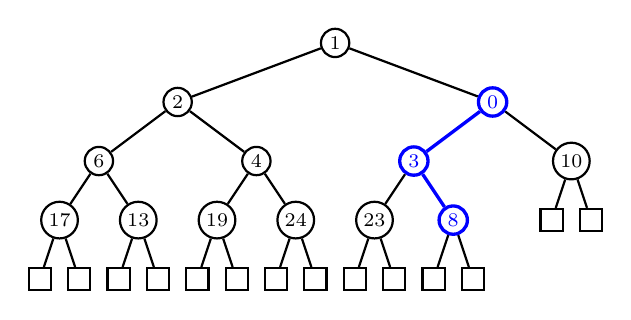
\begin{tikzpicture}
[-,thick,%
  every node/.style={shape=circle,inner sep=1.5pt,draw,thick},%
  scale=0.5]
\scriptsize
\node {$1$}
  [sibling distance=8cm]
  child {node {$2$}
    [sibling distance=4cm]
    child {node {$6$}
      [sibling distance=2cm]
      child {node {$17$}
        [sibling distance=1cm]
        child {node[rectangle,inner sep=4pt,draw,thick] {}}
        child {node[rectangle,inner sep=4pt,draw,thick] {}}
      }
      child {node {$13$}
        [sibling distance=1cm]
        child {node[rectangle,inner sep=4pt,draw,thick] {}}
        child {node[rectangle,inner sep=4pt,draw,thick] {}}
      }
    }
    child {node {$4$}
      [sibling distance=2cm]
      child {node {$19$}
        [sibling distance=1cm]
        child {node[rectangle,inner sep=4pt,draw,thick] {}}
        child {node[rectangle,inner sep=4pt,draw,thick] {}}
      }
      child {node {$24$}
        [sibling distance=1cm]
        child {node[rectangle,inner sep=4pt,draw,thick] {}}
        child {node[rectangle,inner sep=4pt,draw,thick] {}}
      }
    }
  }
  child {node[blue,very thick] {$0$}
    [sibling distance=4cm]
    child[blue,very thick] {node[blue,very thick] {$3$}
      [sibling distance=2cm]
      child[black,thick] {node {$23$}
        [sibling distance=1cm]
        child {node[rectangle,inner sep=4pt,draw,thick] {}}
        child {node[rectangle,inner sep=4pt,draw,thick] {}}
      }
      child[blue,very thick] {node[blue,very thick] {$8$}
        [sibling distance=1cm]
        child[black,thick] {node[rectangle,inner sep=4pt,draw,thick] {}}
        child[black,thick] {node[rectangle,inner sep=4pt,draw,thick] {}}
      }
    }
    child {node {$10$}
      [sibling distance=1cm]
      child {node[rectangle,inner sep=4pt,draw,thick] {}}
      child {node[rectangle,inner sep=4pt,draw,thick] {}}
    }
  };
\end{tikzpicture}
}
%%
%%
\subfigure[]{
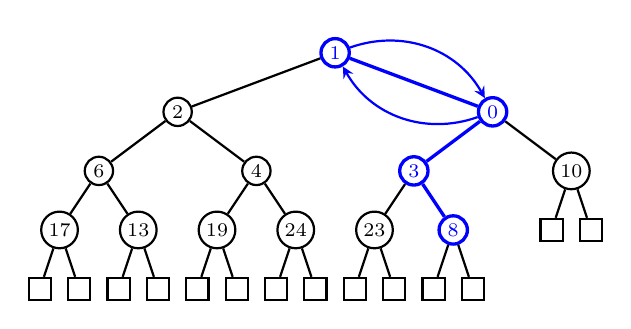
\begin{tikzpicture}
[-,thick,%
  every node/.style={shape=circle,inner sep=1.5pt,draw,thick},%
  scale=0.5]
\scriptsize
\node[blue,very thick] (1) {$1$}
  [sibling distance=8cm]
  child {node {$2$}
    [sibling distance=4cm]
    child {node {$6$}
      [sibling distance=2cm]
      child {node {$17$}
        [sibling distance=1cm]
        child {node[rectangle,inner sep=4pt,draw,thick] {}}
        child {node[rectangle,inner sep=4pt,draw,thick] {}}
      }
      child {node {$13$}
        [sibling distance=1cm]
        child {node[rectangle,inner sep=4pt,draw,thick] {}}
        child {node[rectangle,inner sep=4pt,draw,thick] {}}
      }
    }
    child {node {$4$}
      [sibling distance=2cm]
      child {node {$19$}
        [sibling distance=1cm]
        child {node[rectangle,inner sep=4pt,draw,thick] {}}
        child {node[rectangle,inner sep=4pt,draw,thick] {}}
      }
      child {node {$24$}
        [sibling distance=1cm]
        child {node[rectangle,inner sep=4pt,draw,thick] {}}
        child {node[rectangle,inner sep=4pt,draw,thick] {}}
      }
    }
  }
  child[blue,very thick] {node[blue,very thick] (0) {$0$}
    [sibling distance=4cm]
    child[blue,very thick] {node[blue,very thick] {$3$}
      [sibling distance=2cm]
      child[black,thick] {node {$23$}
        [sibling distance=1cm]
        child {node[rectangle,inner sep=4pt,draw,thick] {}}
        child {node[rectangle,inner sep=4pt,draw,thick] {}}
      }
      child[blue,very thick] {node[blue,very thick] {$8$}
        [sibling distance=1cm]
        child[black,thick] {node[rectangle,inner sep=4pt,draw,thick] {}}
        child[black,thick] {node[rectangle,inner sep=4pt,draw,thick] {}}
      }
    }
    child[black,thick] {node {$10$}
      [sibling distance=1cm]
      child {node[rectangle,inner sep=4pt,draw,thick] {}}
      child {node[rectangle,inner sep=4pt,draw,thick] {}}
    }
  };
\path
(0) edge[->,>=stealth,thick,bend left=40,blue] (1)
(1) edge[->,>=stealth,thick,bend left=40,blue] (0);
\end{tikzpicture}
}
%%
%%
\quad
\subfigure[]{
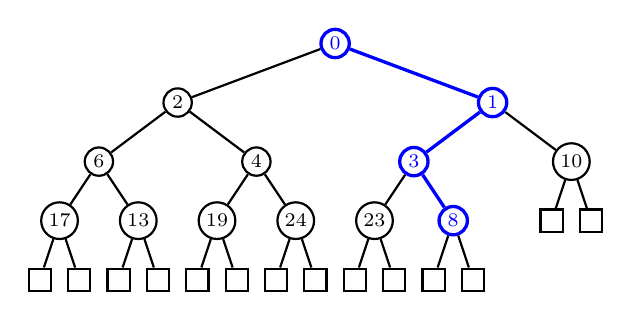
\begin{tikzpicture}
[-,thick,%
  every node/.style={shape=circle,inner sep=1.5pt,draw,thick},%
  scale=0.5]
\scriptsize
\node[blue,very thick] {$0$}
  [sibling distance=8cm]
  child {node {$2$}
    [sibling distance=4cm]
    child {node {$6$}
      [sibling distance=2cm]
      child {node {$17$}
        [sibling distance=1cm]
        child {node[rectangle,inner sep=4pt,draw,thick] {}}
        child {node[rectangle,inner sep=4pt,draw,thick] {}}
      }
      child {node {$13$}
        [sibling distance=1cm]
        child {node[rectangle,inner sep=4pt,draw,thick] {}}
        child {node[rectangle,inner sep=4pt,draw,thick] {}}
      }
    }
    child {node {$4$}
      [sibling distance=2cm]
      child {node {$19$}
        [sibling distance=1cm]
        child {node[rectangle,inner sep=4pt,draw,thick] {}}
        child {node[rectangle,inner sep=4pt,draw,thick] {}}
      }
      child {node {$24$}
        [sibling distance=1cm]
        child {node[rectangle,inner sep=4pt,draw,thick] {}}
        child {node[rectangle,inner sep=4pt,draw,thick] {}}
      }
    }
  }
  child[blue,very thick] {node[blue,very thick] {$1$}
    [sibling distance=4cm]
    child[blue,very thick] {node[blue,very thick] {$3$}
      [sibling distance=2cm]
      child[black,thick] {node {$23$}
        [sibling distance=1cm]
        child {node[rectangle,inner sep=4pt,draw,thick] {}}
        child {node[rectangle,inner sep=4pt,draw,thick] {}}
      }
      child[blue,very thick] {node[blue,very thick] {$8$}
        [sibling distance=1cm]
        child[black,thick] {node[rectangle,inner sep=4pt,draw,thick] {}}
        child[black,thick] {node[rectangle,inner sep=4pt,draw,thick] {}}
      }
    }
    child[black,thick] {node {$10$}
      [sibling distance=1cm]
      child {node[rectangle,inner sep=4pt,draw,thick] {}}
      child {node[rectangle,inner sep=4pt,draw,thick] {}}
    }
  };
\end{tikzpicture}
}

\caption{Insert and sift-up in a binary heap.}
\label{fig:tree_data_structures:insert_sift_up_binary_heap}
\end{figure}

\begin{algorithm}[!htbp]
%%%%%%%%%%%%%%%%%%%%%%%%%%%%%%%%%%%%%%%%%%%%%%%%%%%%%%%%%%%%%%%%%%%%%%%%%%%
%% This file is part of the book
%%
%% Algorithmic Graph Theory
%% http://code.google.com/p/graph-theory-algorithms-book/
%%
%% Copyright (C) 2009, 2010 Minh Van Nguyen <nguyenminh2@gmail.com>
%%
%% See the file COPYING for copying conditions.
%%%%%%%%%%%%%%%%%%%%%%%%%%%%%%%%%%%%%%%%%%%%%%%%%%%%%%%%%%%%%%%%%%%%%%%%%%%

\DontPrintSemicolon
\SetAlgoNoLine
%%
%% data section
\SetKwInOut{Input}{Input}
\SetKwInOut{Output}{Output}
%%
%% input/output
\Input{A nonempty binary heap $T$, in sequence representation, having
  $n$ internal vertices. An element $v$ that is to be inserted as a
  new internal vertex of $T$.}
\Output{The binary heap $T$ augmented with the new internal vertex $v$.}
\BlankLine
%%
%% algorithm body
$i \assign n$\;
\While{$i > 0$}{
  $p \assign \lfloor (i - 1) / 2\rfloor$\;
  \eIf{$\kappa_{T[p]} \leq \kappa_{v}$}{
    exit the loop\;
  }{
    $T[i] \assign T[p]$\;
    $i \assign p$\;
  }
}
$T[i] \assign v$\;
\Return $T$\;

\caption{Inserting a new internal vertex into a binary heap.}
\label{alg:tree_data_structures:binary_heap_insert}
\end{algorithm}


%%%%%%%%%%%%%%%%%%%%%%%%%%%%%%%%%%%%%%%%%%%%%%%%%%%%%%%%%%%%%%%%%%%%%%%%%%%

\subsection{Deletion and sift-down}
\label{subsec:tree_data_structures:deletion_sift_down}

The process for deleting the minimum vertex of a binary heap bears
some resemblance to that of inserting a new internal vertex into the
heap. Having removed the minimum vertex, we must then ensure that the
resulting binary heap satisfies the heap-order property. Let $T$ be a
binary heap. By the heap-order property, the root of $T$ has a key
that is minimum among all keys of internal vertices in $T$. If the
root $r$ of $T$ is the only internal vertex of $T$, i.e. $T$ is the
trivial binary heap, we simply remove $r$ and $T$ now becomes the
empty binary heap or the trivial tree, for which the heap-order
property vacuously holds.
Figure~\ref{fig:tree_data_structures:deleting_root_trivial_binary_heap}
illustrates the case of removing the root of a binary heap having one
internal vertex.

\begin{figure}[!htbp]
\centering
%%%%%%%%%%%%%%%%%%%%%%%%%%%%%%%%%%%%%%%%%%%%%%%%%%%%%%%%%%%%%%%%%%%%%%%%%%%
%% This file is part of the book
%%
%% Algorithmic Graph Theory
%% http://code.google.com/p/graph-theory-algorithms-book/
%%
%% Copyright (C) 2009, 2010, 2011 Minh Van Nguyen <nguyenminh2@gmail.com>
%%
%% See the file COPYING for copying conditions.
%%%%%%%%%%%%%%%%%%%%%%%%%%%%%%%%%%%%%%%%%%%%%%%%%%%%%%%%%%%%%%%%%%%%%%%%%%%

\documentclass{article}

\usepackage{subfigure}
\usepackage{tikz}
\usetikzlibrary{external}
\usetikzlibrary{trees}
\tikzexternalize{binary-heap-delete-empty}

\begin{document}

\begin{figure}
\subfigure[]{
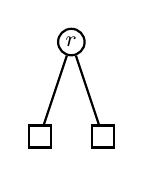
\begin{tikzpicture}
[-,thick,%
  every node/.style={shape=circle,inner sep=1.5pt,draw,thick},%
  scale=0.8]
\footnotesize
\node {$r$}
  [sibling distance=1cm]
  child {node[rectangle,inner sep=4pt,draw,thick] {}}
  child {node[rectangle,inner sep=4pt,draw,thick] {}};
\end{tikzpicture}
}
%%
%%
\qquad
\subfigure[]{
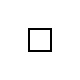
\begin{tikzpicture}
[-,thick,%
  every node/.style={shape=rectangle,inner sep=4pt,draw,thick},%
  scale=0.8]
\footnotesize
\node {};
\end{tikzpicture}
}
\end{figure}

\end{document}

\caption{Deleting the root of a trivial binary heap.}
\label{fig:tree_data_structures:deleting_root_trivial_binary_heap}
\end{figure}

We now turn to the case where $T$ has $n > 1$ internal vertices. Let
$r$ be the root of $T$ and let $v$ be the last internal vertex of
$T$. Deleting $r$ would disconnect $T$. So we instead replace the key
and information at $r$ with the key and other relevant information
pertaining to $v$. The root $r$ now has the key of the last internal
vertex, and $v$ becomes a leaf.

At this point, $T$ satisfies the heap-structure property but may
violate the heap-order property. To restore the heap-order property,
we perform an operation on $T$ called
\emph{sift-down}\index{binary heap!sift-down} that may possibly move
$r$ down through various levels of $T$. Let $c(r)$ be the child of $r$
with key that is minimum among all the children of $r$, and let
$\kappa_r$ and $\kappa_{c(r)}$ be the keys of $r$ and $c(r)$,
respectively. If $\kappa_r \leq \kappa_{c(r)}$, then the heap-order
property is satisfied. Otherwise we swap $r$ with $c(r)$, moving $r$
down one level to the position previously occupied by
$c(r)$. Furthermore, $c(r)$ is moved up one level to the position
previously occupied by $r$. With $r$ in its new position, we perform
the same key comparison process with a child of $r$ that has minimum
key among all of $r$'s children. The key comparison and swapping
continue until the heap-order property holds for $T$. In the worst
case, $r$ would percolate all the way down to the level that is
immediately above the last level after undergoing a number of swaps
that is proportional to the height of $T$. Therefore, deleting the
minimum vertex of $T$ can be achieved in time $O(\lg n)$.
Figure~\ref{fig:tree_data_structures:delete_sift_down_binary_heap}
illustrates the deletion of the minimum vertex of a binary heap with
at least two internal vertices and the resulting sift-down process
that percolates vertices down through various levels of the heap in
order to maintain the heap-order property.
Algorithm~\ref{alg:tree_data_structures:binary_heap_delete} summarizes
our discussion of the process for extracting the minimum vertex of $T$
while also ensuring that $T$ satisfies the heap-order property. The
pseudocode is adapted from the C implementation of binary heaps in
Howard~\cite{Howard2010}. With some minor changes,
Algorithm~\ref{alg:tree_data_structures:binary_heap_delete} can be
used to change the key of the root vertex and maintain the heap-order
property for the resulting binary tree.

\begin{figure}[!htbp]
\centering
%%%%%%%%%%%%%%%%%%%%%%%%%%%%%%%%%%%%%%%%%%%%%%%%%%%%%%%%%%%%%%%%%%%%%%%%%%%
%% This file is part of the book
%%
%% Algorithmic Graph Theory
%% http://code.google.com/p/graph-theory-algorithms-book/
%%
%% Copyright (C) 2009, 2010, 2011 Minh Van Nguyen <nguyenminh2@gmail.com>
%%
%% See the file COPYING for copying conditions.
%%%%%%%%%%%%%%%%%%%%%%%%%%%%%%%%%%%%%%%%%%%%%%%%%%%%%%%%%%%%%%%%%%%%%%%%%%%

\subfigure[]{
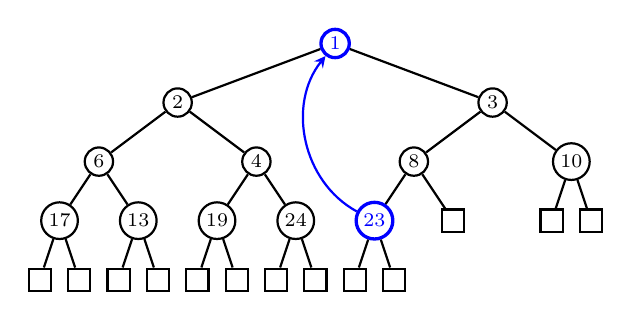
\begin{tikzpicture}
[-,thick,%
  every node/.style={shape=circle,inner sep=1.5pt,draw,thick},%
  scale=0.5]
\scriptsize
\node[blue,very thick] (1) {$1$}
  [sibling distance=8cm]
  child {node {$2$}
    [sibling distance=4cm]
    child {node {$6$}
      [sibling distance=2cm]
      child {node {$17$}
        [sibling distance=1cm]
        child {node[rectangle,inner sep=4pt,draw,thick] {}}
        child {node[rectangle,inner sep=4pt,draw,thick] {}}
      }
      child {node {$13$}
        [sibling distance=1cm]
        child {node[rectangle,inner sep=4pt,draw,thick] {}}
        child {node[rectangle,inner sep=4pt,draw,thick] {}}
      }
    }
    child {node {$4$}
      [sibling distance=2cm]
      child {node {$19$}
        [sibling distance=1cm]
        child {node[rectangle,inner sep=4pt,draw,thick] {}}
        child {node[rectangle,inner sep=4pt,draw,thick] {}}
      }
      child {node {$24$}
        [sibling distance=1cm]
        child {node[rectangle,inner sep=4pt,draw,thick] {}}
        child {node[rectangle,inner sep=4pt,draw,thick] {}}
      }
    }
  }
  child {node {$3$}
    [sibling distance=4cm]
    child {node {$8$}
      [sibling distance=2cm]
      child {node[blue,very thick] (23) {$23$}
        [sibling distance=1cm]
        child {node[rectangle,inner sep=4pt,draw,thick] {}}
        child {node[rectangle,inner sep=4pt,draw,thick] {}}
      }
      child {node[rectangle,inner sep=4pt,draw,thick] {}}
    }
    child {node {$10$}
      [sibling distance=1cm]
      child {node[rectangle,inner sep=4pt,draw,thick] {}}
      child {node[rectangle,inner sep=4pt,draw,thick] {}}
    }
  };
\path
(23) edge[->,>=stealth,thick,bend left=50,blue] (1);
\end{tikzpicture}
}
%%
%%
\quad
\subfigure[]{
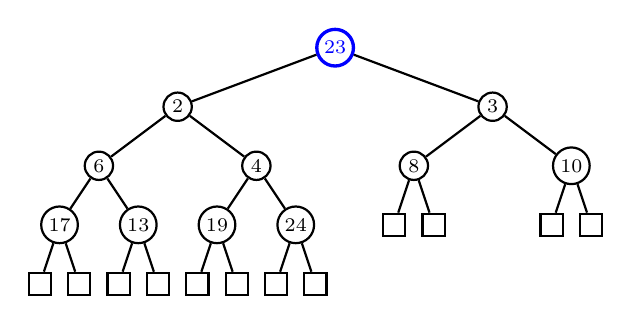
\begin{tikzpicture}
[-,thick,%
  every node/.style={shape=circle,inner sep=1.5pt,draw,thick},%
  scale=0.5]
\scriptsize
\node[blue,very thick] {$23$}
  [sibling distance=8cm]
  child {node {$2$}
    [sibling distance=4cm]
    child {node {$6$}
      [sibling distance=2cm]
      child {node {$17$}
        [sibling distance=1cm]
        child {node[rectangle,inner sep=4pt,draw,thick] {}}
        child {node[rectangle,inner sep=4pt,draw,thick] {}}
      }
      child {node {$13$}
        [sibling distance=1cm]
        child {node[rectangle,inner sep=4pt,draw,thick] {}}
        child {node[rectangle,inner sep=4pt,draw,thick] {}}
      }
    }
    child {node {$4$}
      [sibling distance=2cm]
      child {node {$19$}
        [sibling distance=1cm]
        child {node[rectangle,inner sep=4pt,draw,thick] {}}
        child {node[rectangle,inner sep=4pt,draw,thick] {}}
      }
      child {node {$24$}
        [sibling distance=1cm]
        child {node[rectangle,inner sep=4pt,draw,thick] {}}
        child {node[rectangle,inner sep=4pt,draw,thick] {}}
      }
    }
  }
  child {node {$3$}
    [sibling distance=4cm]
    child {node {$8$}
      [sibling distance=1cm]
      child {node[rectangle,inner sep=4pt,draw,thick] {}}
      child {node[rectangle,inner sep=4pt,draw,thick] {}}
    }
    child {node {$10$}
      [sibling distance=1cm]
      child {node[rectangle,inner sep=4pt,draw,thick] {}}
      child {node[rectangle,inner sep=4pt,draw,thick] {}}
    }
  };
\end{tikzpicture}
}
%%
%%
\subfigure[]{
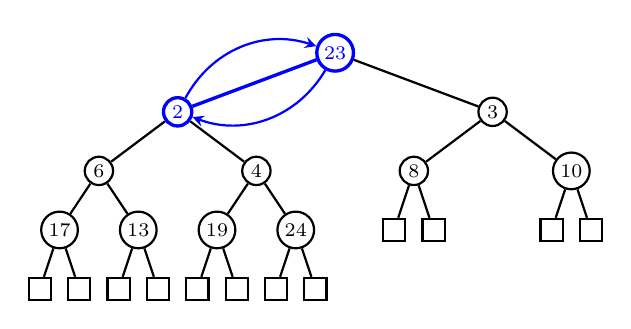
\begin{tikzpicture}
[-,thick,%
  every node/.style={shape=circle,inner sep=1.5pt,draw,thick},%
  scale=0.5]
\scriptsize
\node[blue,very thick] (23) {$23$}
  [sibling distance=8cm]
  child[blue,very thick] {node[blue,very thick] (2) {$2$}
    [sibling distance=4cm]
    child[black,thick] {node {$6$}
      [sibling distance=2cm]
      child {node {$17$}
        [sibling distance=1cm]
        child {node[rectangle,inner sep=4pt,draw,thick] {}}
        child {node[rectangle,inner sep=4pt,draw,thick] {}}
      }
      child {node {$13$}
        [sibling distance=1cm]
        child {node[rectangle,inner sep=4pt,draw,thick] {}}
        child {node[rectangle,inner sep=4pt,draw,thick] {}}
      }
    }
    child[black,thick] {node {$4$}
      [sibling distance=2cm]
      child {node {$19$}
        [sibling distance=1cm]
        child {node[rectangle,inner sep=4pt,draw,thick] {}}
        child {node[rectangle,inner sep=4pt,draw,thick] {}}
      }
      child {node {$24$}
        [sibling distance=1cm]
        child {node[rectangle,inner sep=4pt,draw,thick] {}}
        child {node[rectangle,inner sep=4pt,draw,thick] {}}
      }
    }
  }
  child {node {$3$}
    [sibling distance=4cm]
    child {node {$8$}
      [sibling distance=1cm]
      child {node[rectangle,inner sep=4pt,draw,thick] {}}
      child {node[rectangle,inner sep=4pt,draw,thick] {}}
    }
    child {node {$10$}
      [sibling distance=1cm]
      child {node[rectangle,inner sep=4pt,draw,thick] {}}
      child {node[rectangle,inner sep=4pt,draw,thick] {}}
    }
  };
\path
(2) edge[->,>=stealth,thick,bend left=40,blue] (23)
(23) edge[->,>=stealth,thick,bend left=40,blue] (2);
\end{tikzpicture}
}
%%
%%
\quad
\subfigure[]{
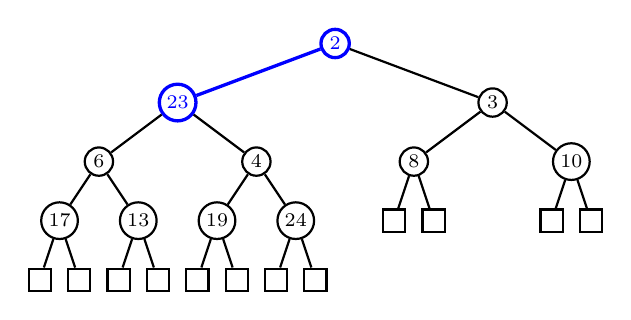
\begin{tikzpicture}
[-,thick,%
  every node/.style={shape=circle,inner sep=1.5pt,draw,thick},%
  scale=0.5]
\scriptsize
\node[blue,very thick] {$2$}
  [sibling distance=8cm]
  child[blue,very thick] {node[blue,very thick] {$23$}
    [sibling distance=4cm]
    child[black,thick] {node {$6$}
      [sibling distance=2cm]
      child {node {$17$}
        [sibling distance=1cm]
        child {node[rectangle,inner sep=4pt,draw,thick] {}}
        child {node[rectangle,inner sep=4pt,draw,thick] {}}
      }
      child {node {$13$}
        [sibling distance=1cm]
        child {node[rectangle,inner sep=4pt,draw,thick] {}}
        child {node[rectangle,inner sep=4pt,draw,thick] {}}
      }
    }
    child[black,thick] {node {$4$}
      [sibling distance=2cm]
      child {node {$19$}
        [sibling distance=1cm]
        child {node[rectangle,inner sep=4pt,draw,thick] {}}
        child {node[rectangle,inner sep=4pt,draw,thick] {}}
      }
      child {node {$24$}
        [sibling distance=1cm]
        child {node[rectangle,inner sep=4pt,draw,thick] {}}
        child {node[rectangle,inner sep=4pt,draw,thick] {}}
      }
    }
  }
  child {node {$3$}
    [sibling distance=4cm]
    child {node {$8$}
      [sibling distance=1cm]
      child {node[rectangle,inner sep=4pt,draw,thick] {}}
      child {node[rectangle,inner sep=4pt,draw,thick] {}}
    }
    child {node {$10$}
      [sibling distance=1cm]
      child {node[rectangle,inner sep=4pt,draw,thick] {}}
      child {node[rectangle,inner sep=4pt,draw,thick] {}}
    }
  };
\end{tikzpicture}
}
%%
%%
\subfigure[]{
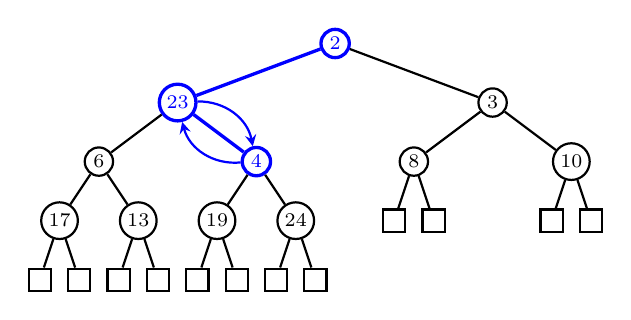
\begin{tikzpicture}
[-,thick,%
  every node/.style={shape=circle,inner sep=1.5pt,draw,thick},%
  scale=0.5]
\scriptsize
\node[blue,very thick] {$2$}
  [sibling distance=8cm]
  child[blue,very thick] {node[blue,very thick] (23) {$23$}
    [sibling distance=4cm]
    child[black,thick] {node {$6$}
      [sibling distance=2cm]
      child {node {$17$}
        [sibling distance=1cm]
        child {node[rectangle,inner sep=4pt,draw,thick] {}}
        child {node[rectangle,inner sep=4pt,draw,thick] {}}
      }
      child {node {$13$}
        [sibling distance=1cm]
        child {node[rectangle,inner sep=4pt,draw,thick] {}}
        child {node[rectangle,inner sep=4pt,draw,thick] {}}
      }
    }
    child[blue,very thick] {node[blue,very thick] (4) {$4$}
      [sibling distance=2cm]
      child[black,thick] {node {$19$}
        [sibling distance=1cm]
        child {node[rectangle,inner sep=4pt,draw,thick] {}}
        child {node[rectangle,inner sep=4pt,draw,thick] {}}
      }
      child[black,thick] {node {$24$}
        [sibling distance=1cm]
        child {node[rectangle,inner sep=4pt,draw,thick] {}}
        child {node[rectangle,inner sep=4pt,draw,thick] {}}
      }
    }
  }
  child {node {$3$}
    [sibling distance=4cm]
    child {node {$8$}
      [sibling distance=1cm]
      child {node[rectangle,inner sep=4pt,draw,thick] {}}
      child {node[rectangle,inner sep=4pt,draw,thick] {}}
    }
    child {node {$10$}
      [sibling distance=1cm]
      child {node[rectangle,inner sep=4pt,draw,thick] {}}
      child {node[rectangle,inner sep=4pt,draw,thick] {}}
    }
  };
\path
(4) edge[->,>=stealth,thick,bend left=40,blue] (23)
(23) edge[->,>=stealth,thick,bend left=40,blue] (4);
\end{tikzpicture}
}
%%
%%
\quad
\subfigure[]{
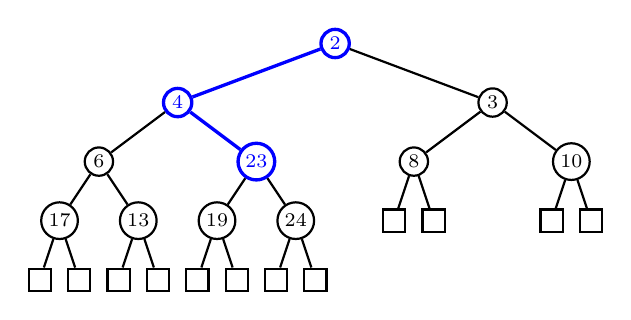
\begin{tikzpicture}
[-,thick,%
  every node/.style={shape=circle,inner sep=1.5pt,draw,thick},%
  scale=0.5]
\scriptsize
\node[blue,very thick] {$2$}
  [sibling distance=8cm]
  child[blue,very thick] {node[blue,very thick] {$4$}
    [sibling distance=4cm]
    child[black,thick] {node {$6$}
      [sibling distance=2cm]
      child {node {$17$}
        [sibling distance=1cm]
        child {node[rectangle,inner sep=4pt,draw,thick] {}}
        child {node[rectangle,inner sep=4pt,draw,thick] {}}
      }
      child {node {$13$}
        [sibling distance=1cm]
        child {node[rectangle,inner sep=4pt,draw,thick] {}}
        child {node[rectangle,inner sep=4pt,draw,thick] {}}
      }
    }
    child[blue,very thick] {node[blue,very thick] {$23$}
      [sibling distance=2cm]
      child[black,thick] {node {$19$}
        [sibling distance=1cm]
        child {node[rectangle,inner sep=4pt,draw,thick] {}}
        child {node[rectangle,inner sep=4pt,draw,thick] {}}
      }
      child[black,thick] {node {$24$}
        [sibling distance=1cm]
        child {node[rectangle,inner sep=4pt,draw,thick] {}}
        child {node[rectangle,inner sep=4pt,draw,thick] {}}
      }
    }
  }
  child {node {$3$}
    [sibling distance=4cm]
    child {node {$8$}
      [sibling distance=1cm]
      child {node[rectangle,inner sep=4pt,draw,thick] {}}
      child {node[rectangle,inner sep=4pt,draw,thick] {}}
    }
    child {node {$10$}
      [sibling distance=1cm]
      child {node[rectangle,inner sep=4pt,draw,thick] {}}
      child {node[rectangle,inner sep=4pt,draw,thick] {}}
    }
  };
\end{tikzpicture}
}
%%
%%
\subfigure[]{
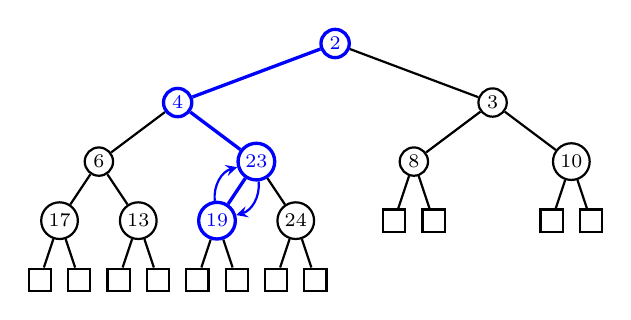
\begin{tikzpicture}
[-,thick,%
  every node/.style={shape=circle,inner sep=1.5pt,draw,thick},%
  scale=0.5]
\scriptsize
\node[blue,very thick] {$2$}
  [sibling distance=8cm]
  child[blue,very thick] {node[blue,very thick] {$4$}
    [sibling distance=4cm]
    child[black,thick] {node {$6$}
      [sibling distance=2cm]
      child {node {$17$}
        [sibling distance=1cm]
        child {node[rectangle,inner sep=4pt,draw,thick] {}}
        child {node[rectangle,inner sep=4pt,draw,thick] {}}
      }
      child {node {$13$}
        [sibling distance=1cm]
        child {node[rectangle,inner sep=4pt,draw,thick] {}}
        child {node[rectangle,inner sep=4pt,draw,thick] {}}
      }
    }
    child[blue,very thick] {node[blue,very thick] (23) {$23$}
      [sibling distance=2cm]
      child[blue,very thick] {node[blue,very thick] (19) {$19$}
        [sibling distance=1cm]
        child[black,thick] {node[rectangle,inner sep=4pt,draw,thick] {}}
        child[black,thick] {node[rectangle,inner sep=4pt,draw,thick] {}}
      }
      child[black,thick] {node {$24$}
        [sibling distance=1cm]
        child {node[rectangle,inner sep=4pt,draw,thick] {}}
        child {node[rectangle,inner sep=4pt,draw,thick] {}}
      }
    }
  }
  child {node {$3$}
    [sibling distance=4cm]
    child {node {$8$}
      [sibling distance=1cm]
      child {node[rectangle,inner sep=4pt,draw,thick] {}}
      child {node[rectangle,inner sep=4pt,draw,thick] {}}
    }
    child {node {$10$}
      [sibling distance=1cm]
      child {node[rectangle,inner sep=4pt,draw,thick] {}}
      child {node[rectangle,inner sep=4pt,draw,thick] {}}
    }
  };
\path
(19) edge[->,>=stealth,thick,bend left=40,blue] (23)
(23) edge[->,>=stealth,thick,bend left=40,blue] (19);
\end{tikzpicture}
}
%%
%%
\quad
\subfigure[]{
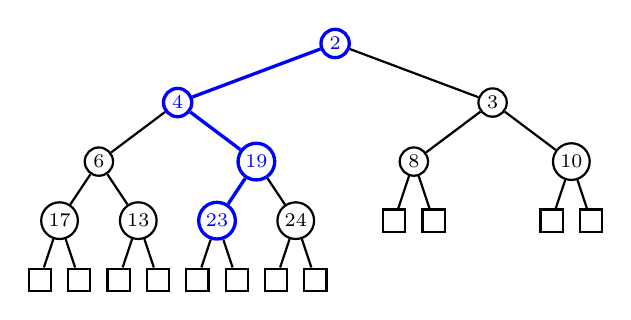
\begin{tikzpicture}
[-,thick,%
  every node/.style={shape=circle,inner sep=1.5pt,draw,thick},%
  scale=0.5]
\scriptsize
\node[blue,very thick] {$2$}
  [sibling distance=8cm]
  child[blue,very thick] {node[blue,very thick] {$4$}
    [sibling distance=4cm]
    child[black,thick] {node {$6$}
      [sibling distance=2cm]
      child {node {$17$}
        [sibling distance=1cm]
        child {node[rectangle,inner sep=4pt,draw,thick] {}}
        child {node[rectangle,inner sep=4pt,draw,thick] {}}
      }
      child {node {$13$}
        [sibling distance=1cm]
        child {node[rectangle,inner sep=4pt,draw,thick] {}}
        child {node[rectangle,inner sep=4pt,draw,thick] {}}
      }
    }
    child[blue,very thick] {node[blue,very thick] {$19$}
      [sibling distance=2cm]
      child[blue,very thick] {node[blue,very thick] {$23$}
        [sibling distance=1cm]
        child[black,thick] {node[rectangle,inner sep=4pt,draw,thick] {}}
        child[black,thick] {node[rectangle,inner sep=4pt,draw,thick] {}}
      }
      child[black,thick] {node {$24$}
        [sibling distance=1cm]
        child {node[rectangle,inner sep=4pt,draw,thick] {}}
        child {node[rectangle,inner sep=4pt,draw,thick] {}}
      }
    }
  }
  child {node {$3$}
    [sibling distance=4cm]
    child {node {$8$}
      [sibling distance=1cm]
      child {node[rectangle,inner sep=4pt,draw,thick] {}}
      child {node[rectangle,inner sep=4pt,draw,thick] {}}
    }
    child {node {$10$}
      [sibling distance=1cm]
      child {node[rectangle,inner sep=4pt,draw,thick] {}}
      child {node[rectangle,inner sep=4pt,draw,thick] {}}
    }
  };
\end{tikzpicture}
}

\caption{Delete and sift-down in a binary heap.}
\label{fig:tree_data_structures:delete_sift_down_binary_heap}
\end{figure}

\begin{algorithm}[!htbp]
%%%%%%%%%%%%%%%%%%%%%%%%%%%%%%%%%%%%%%%%%%%%%%%%%%%%%%%%%%%%%%%%%%%%%%%%%%%
%% This file is part of the book
%%
%% Algorithmic Graph Theory
%% http://code.google.com/p/graph-theory-algorithms-book/
%%
%% Copyright (C) 2009, 2010 Minh Van Nguyen <nguyenminh2@gmail.com>
%%
%% See the file COPYING for copying conditions.
%%%%%%%%%%%%%%%%%%%%%%%%%%%%%%%%%%%%%%%%%%%%%%%%%%%%%%%%%%%%%%%%%%%%%%%%%%%

\DontPrintSemicolon
\SetAlgoNoLine
%%
%% data section
\SetKwInOut{Input}{Input}
\SetKwInOut{Output}{Output}
\SetKwData{MyLeft}{left}
\SetKwData{MyRight}{right}
\SetKwData{MyRoot}{root}
\SetKwData{MyTrue}{true}
%%
%% input/output
\Input{A binary heap $T$, given in sequence representation, having
  $n > 1$ internal vertices.}
\Output{Extract the minimum vertex of $T$. With one vertex removed,
  $T$ must satisfy the heap-order property.}
\BlankLine
%%
%% algorithm body
$\MyRoot \assign T[0]$\;
$n \assign n - 1$\;
$v \assign T[n]$\;
$i \assign 0$\;
$j \assign 0$\;
\While{$\MyTrue$}{
  $\MyLeft \assign 2i + 1$\;
  $\MyRight \assign 2i + 2$\;
  \If{\rm $\MyLeft < n$ and $\kappa_{T[\MyLeft]} \leq \kappa_v$}{
    \eIf{\rm $\MyRight < n$ and $\kappa_{T[\MyRight]} \leq \kappa_{T[\MyLeft]}$}{
      $j \assign \MyRight$\;
    }{
      $j \assign \MyLeft$\;
    }
  }
  \ElseIf{\rm $\MyRight < n$ and $\kappa_{T[\MyRight]} \leq \kappa_v$}{
    $j \assign \MyRight$\;
  }
  \Else{
    $T[i] \assign v$\;
    exit the loop\;
  }
  $T[i] \assign T[j]$\;
  $i \assign j$\;
}
\Return $\MyRoot$\;

\caption{Extract the minimum vertex of a binary heap.}
\label{alg:tree_data_structures:binary_heap_delete}
\end{algorithm}


%%%%%%%%%%%%%%%%%%%%%%%%%%%%%%%%%%%%%%%%%%%%%%%%%%%%%%%%%%%%%%%%%%%%%%%%%%%

\subsection{Constructing a binary heap}

Given a collection of $n$ vertices $v_0, v_1, \dots, v_{n-1}$ with
corresponding keys $\kappa_0, \kappa_1, \dots, \kappa_{n-1}$, we want
to construct a binary heap containing exactly those vertices. A basic
approach is to start with a trivial tree and build up a binary heap
via successive insertions. As each insertion requires $O(\lg n)$ time,
the method of binary heap construction via successive insertion of
each of the $n$ vertices requires $O(n \cdot \lg n)$ time. It turns
out we could do a bit better and achieve the same result in linear
time.

\begin{algorithm}[!htbp]
%%%%%%%%%%%%%%%%%%%%%%%%%%%%%%%%%%%%%%%%%%%%%%%%%%%%%%%%%%%%%%%%%%%%%%%%%%%
%% This file is part of the book
%%
%% Algorithmic Graph Theory
%% http://code.google.com/p/graph-theory-algorithms-book/
%%
%% Copyright (C) 2009, 2010, 2011 Minh Van Nguyen <nguyenminh2@gmail.com>
%%
%% See the file COPYING for copying conditions.
%%%%%%%%%%%%%%%%%%%%%%%%%%%%%%%%%%%%%%%%%%%%%%%%%%%%%%%%%%%%%%%%%%%%%%%%%%%

\DontPrintSemicolon
\SetAlgoNoLine
%%
%% data section
\SetKwInOut{Input}{Input}
\SetKwInOut{Output}{Output}
\SetKwData{MyLeft}{left}
\SetKwData{MyRight}{right}
\SetKwData{MyTrue}{true}
%%
%% input/output
\Input{A binary tree $T$, given in sequence representation, having
  $n > 1$ internal vertices.}
\Output{The binary tree $T$ heapified so that it satisfies the
  heap-order property.}
\BlankLine
%%
%% algorithm body
\For{$i \assign \lfloor n/2 \rfloor - 1, \dots, 0$}{
  $v \assign T[i]$\;
  $j \assign 0$\;
  \While{$\MyTrue$}{
    $\MyLeft \assign 2i + 1$\;
    $\MyRight \assign 2i + 2$\;
    \If{\rm $\MyLeft < n$ and $\kappa_{T[\MyLeft]} \leq \kappa_v$}{
      \eIf{\rm $\MyRight < n$ and $\kappa_{T[\MyRight]} \leq \kappa_{T[\MyLeft]}$}{
        $j \assign \MyRight$\;
      }{
        $j \assign \MyLeft$\;
      }
    }
    \ElseIf{\rm $\MyRight < n$ and $\kappa_{T[\MyRight]} \leq \kappa_v$}{
      $j \assign \MyRight$\;
    }
    \Else{
      $T[i] \assign v$\;
      exit the while loop\;
    }
    $T[i] \assign T[j]$\;
    $i \assign j$\;
  }
}
\Return $T$\;

\caption{Heapify a binary tree.}
\label{alg:tree_data_structures:heapify_binary_tree}
\end{algorithm}

A better approach starts by letting $v_0, v_1, \dots, v_{n-1}$ be the
internal vertices of a binary tree $T$. The tree $T$ need not satisfy
the heap-order property, but it must satisfy the heap-structure
property. Suppose $T$ is given in sequence representation so that we
have the correspondence $v_i = T[i]$ and the last internal vertex of
$T$ has index $n - 1$. The parent of $T[n-1]$ has index
\[
j
=
\left\lfloor \frac{n - 1}{2} \right\rfloor.
\]
Any vertex of $T$ with sequence index beyond $n - 1$ is a leaf. In
other words, if an internal vertex has index $> j$, then the children
of that vertex are leaves and have indices $\geq n$. Thus any internal
vertex with index $\geq \lfloor n/2 \rfloor$ has leaves for its
children. Conclude that internal vertices with indices
%%
\begin{equation}
\label{eqn:tree_data_structures:index_internal_vertices_with_leaves}
\left\lfloor \frac{n}{2} \right\rfloor,\,
\left\lfloor \frac{n}{2} \right\rfloor + 1,\,
\left\lfloor \frac{n}{2} \right\rfloor + 2,
\dots,
n - 1.
\end{equation}
%%
have only leaves for their children.

Our next task is to ensure that the heap-order property holds for
$T$. If $v$ is an internal vertex with index
in~\eqref{eqn:tree_data_structures:index_internal_vertices_with_leaves},
then the subtree rooted at $v$ is trivially a binary heap. Consider
the indices from $\lfloor n / 2 \rfloor - 1$ all the way down to
$0$ and let $i$ be such an index, i.e. let
$0 \leq i \leq \lfloor n / 2 \rfloor - 1$. We heapify the subtree of
$T$ rooted at $T[i]$, effectively performing a sift-down on this
subtree. Once we have heapified all subtrees rooted at $T[i]$ for
$0 \leq i \leq \lfloor n / 2 \rfloor - 1$, the resulting tree $T$ is a
binary heap. Our discussion is summarized in
Algorithm~\ref{alg:tree_data_structures:heapify_binary_tree}.

Earlier in this section, we claimed that
Algorithm~\ref{alg:tree_data_structures:heapify_binary_tree} can be
used to construct a binary heap in worst-case linear time. To prove
this, let $T$ be a binary tree satisfying the heap-structure property
and having $n$ internal vertices. By
Corollary~\ref{cor:tree_data_structures:height_binary_heap}, $T$ has
height $h = \lceil \lg(n + 1) \rceil$. We perform a sift-down for at
most $2^i$ vertices of depth $i$, where each sift-down for a subtree
rooted at a vertex of depth $i$ takes $O(h - i)$ time. Then the total
time for Algorithm~\ref{alg:tree_data_structures:heapify_binary_tree}
is
%%
\begin{align*}
O\left( \sum_{0 \leq i < h} 2^i (h - i) \right)
&=
O\left( 2^h \sum_{0 \leq i < h} \frac{2 - i} {2^{h - i}} \right) \\[4pt]
&=
O\left( 2^h \sum_{k > 0} \frac{k}{2^k} \right) \\[4pt]
&=
O\left( 2^{h + 1} \right) \\[4pt]
&=
O(n)
\end{align*}
%%
where we used the closed form $\sum_{k > 0} k / 2^k = 2$ for a
geometric series and
Theorem~\ref{thm:trees_forests:complete_binary_tree_exact_order}.


%%%%%%%%%%%%%%%%%%%%%%%%%%%%%%%%%%%%%%%%%%%%%%%%%%%%%%%%%%%%%%%%%%%%%%%%%%%

\section{Binomial heaps}
\label{sec:tree_data_structures:binomial_heaps}
\index{binomial heap}

We are given two binary heaps $T_1$ and $T_2$ and we want to merge
them into a single heap. We could start by choosing to insert each
element of $T_2$ into $T_1$, successively extracting the minimum
element from $T_2$ and insert that minimum element into $T_1$. If
$T_1$ and $T_2$ have $m$ and $n$ elements, respectively, we would
perform $n$ extractions from $T_2$ totalling
\[
O\left( \sum_{0 < k \leq n} \lg k \right)
\]
time and inserting all of the extracted elements from $T_2$ into
$T_1$ requires a total runtime of
%%
\begin{equation}
\label{eqn:tree_data_structures:total_runtime_inserting_n_extra_elements}
O\left( \sum_{n \leq k < n + m} \lg k \right).
\end{equation}
%%
We approximate the addition of the two sums by
\[
\int_0^{n + m} \lg k \; dk
=
\left. \frac{k \cdot \ln k - k} {\ln 2} + C \right|_{k=0}^{k=n+m}
\]
for some constant $C$. The above method of successive extraction and
insertion therefore has a total runtime of
\[
O\left( \frac{(n + m) \cdot \ln(n + m) - n - m} {\ln 2} \right)
\]
for merging two binary heaps.

Alternatively, we could slightly improve the latter runtime for
merging $T_1$ and $T_2$ by successively extracting the last internal
vertex of $T_2$. The whole process of extracting all elements from
$T_2$ in this way takes $O(n)$ time and inserting each of the
extracted elements into $T_1$ still requires the runtime in
expression~\eqref{eqn:tree_data_structures:total_runtime_inserting_n_extra_elements}.
We approximate the sum
in~\eqref{eqn:tree_data_structures:total_runtime_inserting_n_extra_elements}
by
\[
\int_{k=n}^{k=n+m} \lg k \; dk
=
\left. \frac{k \cdot \ln k - k} {\ln 2} + C \right|_{k=n}^{k=n+m}
\]
for some constant $C$. Therefore the improved extraction and
insertion method requires
\[
O\left(
\frac{(n+m) \cdot \ln(n+m) - n \cdot \ln n - m} {\ln 2} - n
\right)
\]
time in order to merge $T_1$ and $T_2$.

Can we improve on the latter runtime for merging two binary heaps? It
turns out we can by using a type of mergeable heap called
binomial\index{binomial heap} heap that supports merging two heaps in
logarithmic time.


%%%%%%%%%%%%%%%%%%%%%%%%%%%%%%%%%%%%%%%%%%%%%%%%%%%%%%%%%%%%%%%%%%%%%%%%%%%

\subsection{Binomial trees}
\index{binomial tree}

A binomial heap can be considered as a collection of binomial
trees. The binomial tree of order $k$ is denoted $B_k$ and defined
recursively as follows:
%%
\begin{enumerate}
\item The binomial tree of order $0$ is the trivial tree.

\item The binomial tree of order $k > 0$ is a rooted tree, where from
  left to right the children of the root of $B_k$ are roots of
  $B_{k-1}, B_{k-2}, \dots, B_0$.
\end{enumerate}
%%
Various examples of binomial trees are shown in
Figure~\ref{fig:tree_data_structures:binomial_trees_k0_4}. The
binomial tree $B_k$ can also be defined as follows. Let $T_1$ and
$T_2$ be two copies of $B_{k-1}$ with root vertices $r_1$ and $r_2$,
respectively. Then $B_k$ is obtained by letting, say, $r_1$ be the
left-most child of $r_2$.
Lemma~\ref{lem:tree_data_structures:basic_properties_binomial_trees}
lists various basic properties of binomial trees. Property~(3) of
Lemma~\ref{lem:tree_data_structures:basic_properties_binomial_trees}
uses the binomial\index{binomial coefficient} coefficient, from whence
$B_k$ derives its name.

\begin{figure}[!htbp]
\centering
\input{image/tree-data-structures/binomial-trees-order-0-5.tex}
\caption{Binomial trees $B_k$ for $k = 0, 1, 2, 3, 4, 5$.}
\label{fig:tree_data_structures:binomial_trees_k0_4}
\end{figure}

\begin{lemma}
\label{lem:tree_data_structures:basic_properties_binomial_trees}
\textbf{Basic properties of binomial trees.}
Let $B_k$ be a binomial tree of order $k \geq 0$. Then the following
properties hold:
%%
\begin{enumerate}
\item The order of $B_k$ is $2^k$.

\item The height of $B_k$ is $k$.

\item For $0 \leq i \leq k$, we have $\binom{k}{i}$ vertices at depth
  $i$.

\item The root of $B_k$ is the only vertex with maximum degree
  $\Delta(B_k) = k$. If the children of the root are numbered
  $k - 1, k - 2, \dots, 0$ from left to right, then child $i$ is the
  root of the subtree $B_i$.
\end{enumerate}
\end{lemma}

\begin{proof}
We use induction on $k$. The base case for each of the above
properties is $B_0$, which trivially holds.

(1)~By our inductive hypothesis, $B_{k-1}$ has order $2^{k-1}$. Since
$B_k$ is comprised of two copies of $B_{k-1}$, conclude that $B_k$ has
order
\[
2^{k-1} + 2^{k-1}
=
2^k.
\]

(2)~The binomial tree $B_k$ is comprised of two copies of $B_{k-1}$,
the root of one copy being the left-most child of the root of the
other copy. Then the height of $B_k$ is one greater than the height of
$B_{k-1}$. By our inductive hypothesis, $B_{k-1}$ has height $k - 1$
and therefore $B_k$ has height $(k - 1) + 1 = k$.

(3)~Denote by $D(k,i)$ the number of vertices of depth $i$ in
$B_k$. As $B_k$ is comprised of two copies of $B_{k-1}$, a vertex at
depth $i$ in $B_{k-1}$ appears once in $B_k$ at depth $i$ and a second
time at depth $i + 1$. By our inductive hypothesis,
%%
\begin{align*}
D(k,i)
&=
D(k-1, i) + D(k-1, i-1) \\[4pt]
&=
\binom{k-1}{i} + \binom{k-1}{i-1} \\[4pt]
&=
\binom{k}{i}
\end{align*}
%%
where we used Pascal's\index{Pascal!formula} formula which states that
\[
\binom{n+1}{r}
=
\binom{n}{r-1} + \binom{n}{r}
\]
for any positive integers $n$ and $r$ with $r \leq n$.

(4)~This property follows from the definition of $B_k$.
\end{proof}

\begin{corollary}
If a binomial tree has order $n \geq 0$, then the degree of any vertex
$i$ is bounded by $\deg(i) \leq \lg n$.
\end{corollary}

\begin{proof}
Apply properties~(1) and~(4) of
Lemma~\ref{lem:tree_data_structures:basic_properties_binomial_trees}.
\end{proof}


%%%%%%%%%%%%%%%%%%%%%%%%%%%%%%%%%%%%%%%%%%%%%%%%%%%%%%%%%%%%%%%%%%%%%%%%%%%

\subsection{Binomial heaps}
\index{binomial heap}

In 1978, Jean\index{Vuillemin, Jean} Vuillemin~\cite{Vuillemin1978}
introduced binomial heaps as a data structure for implementing
priority queues. Mark~R.~Brown~\cite{Brown1977,Brown1978} subsequently
extended Vuillemin's work, providing detailed analysis of binomial
heaps and introducing an efficient implementation.

A binomial\index{binomial heap} heap $H$ can be considered as a
collection of binomial trees. Each vertex in $H$ has a corresponding
key and all vertex keys of $H$ belong to a totally ordered set having
total order $\leq$. The heap also satisfies the following
\emph{binomial heap properties}\index{binomial heap!properties}:
%%
\begin{itemize}
\item \textbf{Heap-order property.}\index{binomial heap!order property}
  Let $B_k$ be a binomial tree in $H$. If $v$ is a vertex of $B_k$
  other than the root and $p$ is the parent of $v$ and having
  corresponding keys $\kappa_v$ and $\kappa_p$, respectively, then
  $\kappa_p \leq \kappa_v$.

\item \textbf{Root-degree property.}\index{binomial heap!root-degree property}
  For any integer $k \geq 0$, $H$ contains at most one binomial tree
  whose root has degree $k$.
\end{itemize}

\begin{figure}[!htbp]
\centering
%%%%%%%%%%%%%%%%%%%%%%%%%%%%%%%%%%%%%%%%%%%%%%%%%%%%%%%%%%%%%%%%%%%%%%%%%%%
%% This file is part of the book
%%
%% Algorithmic Graph Theory
%% http://code.google.com/p/graph-theory-algorithms-book/
%%
%% Copyright (C) 2009, 2010 Minh Van Nguyen <nguyenminh2@gmail.com>
%%
%% See the file COPYING for copying conditions.
%%%%%%%%%%%%%%%%%%%%%%%%%%%%%%%%%%%%%%%%%%%%%%%%%%%%%%%%%%%%%%%%%%%%%%%%%%%

\subfigure[Binomial heap as a forest.]{
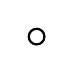
\begin{tikzpicture}
[-,thick,%
  every node/.style={shape=circle,inner sep=2pt,draw,thick}]
\node {};
\end{tikzpicture}
%%
%%
\qquad
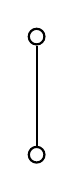
\begin{tikzpicture}
[-,thick,%
  every node/.style={shape=circle,inner sep=2pt,draw,thick}]
\node {}
  child {node {}};
\end{tikzpicture}
%%
%%
\qquad
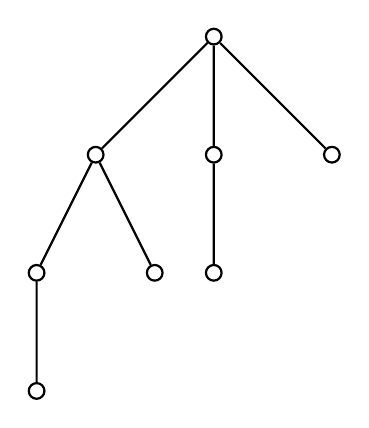
\begin{tikzpicture}
[-,thick,%
  every node/.style={shape=circle,inner sep=2pt,draw,thick}]
\node {}
  child {node {}
    child {node {}
      child {node {}}
    }
    child {node {}}
  }
  child {node {}
    child {node {}}
  }
  child {node {}};
\end{tikzpicture}
}
%%
%%
\qquad
\subfigure[Binomial heap as a tree.]{
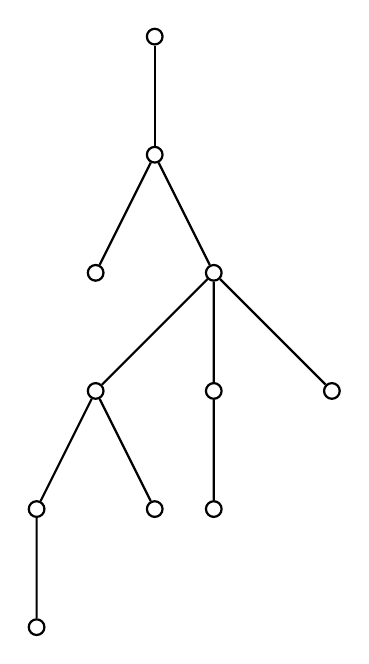
\begin{tikzpicture}
[-,thick,%
  every node/.style={shape=circle,inner sep=2pt,draw,thick}]
\node {}
  child {node {}
    child {node {}}
    child {node{}
      child {node {}
        child {node {}
          child {node {}}
        }
        child {node {}}
      }
      child {node {}
        child {node {}}
      }
      child {node {}}
    }
  };
\end{tikzpicture}
}

\caption{Forest and tree representations of a binomial heap.}
\label{fig:tree_data_structures:binomial_heap_forest_tree_representations}
\end{figure}

If $H$ is comprised of the binomial trees
$B_{k_0}, B_{k_1}, \dots, B_{k_n}$ for nonnegative integers $k_i$, we
can consider $H$ as a forest made up of the trees $B_{k_i}$. We can
also represent $H$ as a tree in the following way. List the binomial
trees of $H$ as $B_{k_0}, B_{k_1}, \dots, B_{k_n}$ in nondecreasing
order of root degrees, i.e. the root of $B_{k_i}$ has order less than
or equal to the root of $B_{k_j}$ if and only if $k_i \leq k_j$. The
root of $H$ is the root of $B_{k_0}$ and the root of each $B_{k_i}$
has for its child the root of $B_{k_{i+1}}$. Both the forest and tree
representations are illustrated in
Figure~\ref{fig:tree_data_structures:binomial_heap_forest_tree_representations}
for the binomial heap comprised of the binomial trees
$B_0, B_1, B_3$.

The heap-order\index{binomial heap!order property} property for
binomial heaps is analogous to the heap-order property for binary
heaps. In the case of binomial heaps, the heap-order property implies
that the root of a binomial tree has a key that is minimum among all
vertices in that tree. However, the similarity more or less ends
there. In a tree representation of a binomial heap, the root of the
heap may not necessarily have the minimum key among all vertices of
the heap.

The root-degree\index{binomial heap!root-degree property} property can
be used to derive an upper bound on the number of binomial trees in a
binomial heap. If $H$ is a binomial heap with $n$ vertices, then $H$
has at most $1 + \lfloor \lg n \rfloor$ binomial trees. To prove this
result, note that~(see Theorem~2.1 and Corollary~2.1.1
in~\cite[pp.40--42]{Rosen2000}) $n$ can be uniquely written in binary
representation as the polynomial
\[
n
=
a_k 2^k + a_{k-1} 2^{k-1} + \cdots + a_1 2^1 + a_0 2^0.
\]
The binary representation of $n$ requires $1 + \lfloor \lg n \rfloor$
bits, hence $n = \sum_{i=0}^{\lfloor \lg n \rfloor} a_i 2^i$. Apply
property~(1) of
Lemma~\ref{lem:tree_data_structures:basic_properties_binomial_trees}
to see that the binomial tree $B_i$ is in $H$ if and only if the
$i$-th bit is $b_i = 1$. Conclude that $H$ has at most
$1 + \lfloor \lg n \rfloor$ binomial trees.


%%%%%%%%%%%%%%%%%%%%%%%%%%%%%%%%%%%%%%%%%%%%%%%%%%%%%%%%%%%%%%%%%%%%%%%%%%%

\subsection{Construction and management}

Let $H$ be a binomial heap comprised of the binomial trees
$B_{k_0}, B_{k_1}, \dots, B_{k_n}$ where the root of $B_{k_i}$ has
order less than or equal to the root of $B_{k_j}$ if and only if
$k_i \leq k_j$. Denote by $r_{k_i}$ the root of the binomial tree
$B_{k_i}$. If $v$ is a vertex of $H$, denote by $\child[v]$ the
left-most child of $v$ and by $\sibling[v]$ we mean the sibling
immediately to the right of $v$. Furthermore, let $\parent[v]$ be the
parent of $v$ and let $\degree[v]$ denote the degree of $v$. If $v$
has no children, we set $\child[v] = \texttt{NULL}$. If $v$ is one of
the roots $r_{k_i}$, we set $\parent[v] = \texttt{NULL}$. And if $v$
is the right-most child of its parent, then we set
$\sibling[v] = \texttt{NULL}$.

The roots $r_{k_0}, r_{k_1}, \dots, r_{k_n}$ can be organized as a
linked list, called a \emph{root list}\index{root list}, with two
functions for accessing the next root and the previous root. The root
immediately following $r_{k_i}$ is denoted
$\nextElem[r_{k_i}] = \sibling[v] = r_{k_{i+1}}$ and the root
immediately before $r_{k_i}$ is written
$\prevElem[r_{k_i}] = r_{k_{i-1}}$. For $r_{k_0}$ and $r_{k_n}$, we
set $\nextElem[r_{k_n}] = \sibling[v] = \texttt{NULL}$ and
$\prevElem[r_{k_0}] = \texttt{NULL}$. We also define the function
$\headElem[H]$ that simply returns $r_{k_0}$ whenever $H$ has at least
one element, and $\headElem[H] = \texttt{NULL}$ otherwise.


%%%%%%%%%%%%%%%%%%%%%%%%%%%%%%%%%%%%%%%%%%%%%%%%%%%%%%%%%%%%%%%%%%%%%%%%%%%

\subsubsection{Minimum vertex}

To find the minimum vertex, we find the minimum among
$r_{k_0}, r_{k_1}, \dots, r_{k_m}$ because by definition the root
$r_{k_i}$ is the minimum vertex of the binomial tree $B_{k_i}$. If $H$
has $n$ vertices, we need to check at most $1 + \lfloor \lg n \rfloor$
vertices to find the minimum vertex of $H$. Therefore determining the
minimum vertex of $H$ takes $O(\lg n)$ time.
Algorithm~\ref{alg:tree_data_structures:binomial_heap_minimum_vertex}
summarizes our discussion.

\begin{algorithm}[!htbp]
%%%%%%%%%%%%%%%%%%%%%%%%%%%%%%%%%%%%%%%%%%%%%%%%%%%%%%%%%%%%%%%%%%%%%%%%%%%
%% This file is part of the book
%%
%% Algorithmic Graph Theory
%% http://code.google.com/p/graph-theory-algorithms-book/
%%
%% Copyright (C) 2009, 2010, 2011 Minh Van Nguyen <nguyenminh2@gmail.com>
%%
%% See the file COPYING for copying conditions.
%%%%%%%%%%%%%%%%%%%%%%%%%%%%%%%%%%%%%%%%%%%%%%%%%%%%%%%%%%%%%%%%%%%%%%%%%%%

\DontPrintSemicolon
\SetAlgoNoLine
%%
%% data section
\SetKwData{MyMin}{min}
\SetKwData{NULL}{\footnotesize{NULL}}
%%
%% input
\KwIn{A binomial heap $H$ of order $n > 0$.}
%%
%% output
\KwOut{The minimum vertex of $H$.}
\BlankLine
%%
%% algorithm body
$u \assign \NULL$\;
$v \assign \headElem[H]$\;
$\MyMin \assign \infty$\;
\While{$v \neq \NULL$}{
  \If{$\kappa_v < \MyMin$}{
    $\MyMin \assign \kappa_v$\;
    $u \assign v$\;
  }
  $v \assign \sibling[v]$\;
}
\Return $u$\;

\caption{Determine the minimum vertex of a binomial heap.}
\label{alg:tree_data_structures:binomial_heap_minimum_vertex}
\end{algorithm}


%%%%%%%%%%%%%%%%%%%%%%%%%%%%%%%%%%%%%%%%%%%%%%%%%%%%%%%%%%%%%%%%%%%%%%%%%%%

\subsubsection{Merging heaps}

Recall that $B_k$ is constructed by linking the root of one copy of
$B_{k-1}$ with the root of another copy of $B_{k-1}$. When merging two
binomial heaps whose roots have the same degree, we need to repeatedly
link the respective roots. The root linking procedure runs in constant
time $O(1)$ and is rather straightforward, as presented in
Algorithm~\ref{alg:tree_data_structures:link_roots}.

\begin{algorithm}[!htbp]
%%%%%%%%%%%%%%%%%%%%%%%%%%%%%%%%%%%%%%%%%%%%%%%%%%%%%%%%%%%%%%%%%%%%%%%%%%%
%% This file is part of the book
%%
%% Algorithmic Graph Theory
%% http://code.google.com/p/graph-theory-algorithms-book/
%%
%% Copyright (C) 2009, 2010, 2011 Minh Van Nguyen <nguyenminh2@gmail.com>
%%
%% See the file COPYING for copying conditions.
%%%%%%%%%%%%%%%%%%%%%%%%%%%%%%%%%%%%%%%%%%%%%%%%%%%%%%%%%%%%%%%%%%%%%%%%%%%

\DontPrintSemicolon
\SetAlgoNoLine
%%
%% data section
\SetKwInOut{Input}{Input}
\SetKwInOut{Output}{Output}
%%
%% input/output
\Input{Two copies of $B_{k-1}$, one rooted at $u$ and the other at $v$.}
\Output{The respective roots of two copies of $B_{k-1}$ linked, with
  one root becoming the parent of the other.}
\BlankLine
%%
%% algorithm body
$\parent[u] \assign v$\;
$\sibling[u] \assign \child[v]$\;
$\child[v] \assign u$\;
$\degree[v] \assign \degree[v] + 1$\;

\caption{Linking the roots of binomial heaps.}
\label{alg:tree_data_structures:link_roots}
\end{algorithm}

Besides linking the roots of two copies of $B_{k-1}$, we also need to
merge the root lists of two binomial heaps $H_1$ and $H_2$. The
resulting merged list is sorted in nondecreasing order of degree. Let
$L_1$ be the root list of $H_1$ and let $L_2$ be the root list of
$H_2$. First we create an empty list $L$. As the lists $L_i$ are
already sorted in nondecreasing order of vertex degree, we use
merge\index{merge sort} sort to merge the $L_i$ into a single sorted
list. The whole procedure for merging the $L_i$ takes linear time
$O(n)$, where $n = |L_1| + |L_2| - 1$. Refer to
Algorithm~\ref{alg:tree_data_structures:merge_root_lists} for
pseudocode of the procedure just described.

\begin{algorithm}[!htbp]
%%%%%%%%%%%%%%%%%%%%%%%%%%%%%%%%%%%%%%%%%%%%%%%%%%%%%%%%%%%%%%%%%%%%%%%%%%%
%% This file is part of the book
%%
%% Algorithmic Graph Theory
%% http://code.google.com/p/graph-theory-algorithms-book/
%%
%% Copyright (C) 2009--2011 Minh Van Nguyen <nguyenminh2@gmail.com>
%%
%% See the file COPYING for copying conditions.
%%%%%%%%%%%%%%%%%%%%%%%%%%%%%%%%%%%%%%%%%%%%%%%%%%%%%%%%%%%%%%%%%%%%%%%%%%%

\DontPrintSemicolon
\SetAlgoNoLine
%%
%% input
\KwIn{Two root lists $L_1$ and $L_2$, each containing the roots of
  binomial trees in the binomial heaps $H_1$ and $H_2$,
  respectively. Each root list $L_i$ is sorted in increasing order of
  vertex degree.}
%%
%% output
\KwOut{A single list $L$ that merges the root lists $L_i$ and sorted
  in nondecreasing order of degree.}
\BlankLine
%%
%% algorithm body
$i \assign 1$\;
$j \assign 1$\;
$L \assign [\,]$\;
$n \assign |L_1| + |L_2| - 1$\;
$\append(L_1,\, \infty)$\;
$\append(L_2,\, \infty)$\;
\For{$k \assign 0, 1, \dots, n$}{
  \If{$\deg(L_1[i]) \leq \deg(L_2[j])$}{
    $\append(L,\, L_1[i])$\;
    $i \assign i + 1$\;
  }
  \Else{
    $\append(L,\, L_2[j])$\;
    $j \assign j + 1$\;
  }
}
\Return $L$\;

\caption{Merging two root lists.}
\label{alg:tree_data_structures:merge_root_lists}
\end{algorithm}

\begin{algorithm}[!htbp]
%%%%%%%%%%%%%%%%%%%%%%%%%%%%%%%%%%%%%%%%%%%%%%%%%%%%%%%%%%%%%%%%%%%%%%%%%%%
%% This file is part of the book
%%
%% Algorithmic Graph Theory
%% http://code.google.com/p/graph-theory-algorithms-book/
%%
%% Copyright (C) 2009, 2010 Minh Van Nguyen <nguyenminh2@gmail.com>
%%
%% See the file COPYING for copying conditions.
%%%%%%%%%%%%%%%%%%%%%%%%%%%%%%%%%%%%%%%%%%%%%%%%%%%%%%%%%%%%%%%%%%%%%%%%%%%

\DontPrintSemicolon
\SetAlgoNoLine
%%
%% data section
\SetKwInOut{Input}{Input}
\SetKwInOut{Output}{Output}
\SetKwData{MyNextV}{nextv}
\SetKwData{MyPrevV}{prevv}
%%
%% input/output
\Input{Two binomial heaps $H_1$ and $H_2$.}
\Output{A binomial heap $H$ that results from merging the $H_i$.}
\BlankLine
%%
%% algorithm body
$H \assign$ empty binomial heap\;
$\headElem[H] \assign$ merge sort the root lists of $H_1$ and $H_2$\;
\If{\rm $\headElem[H] = \texttt{NULL}$}{
  \Return $H$\;
}
$\MyPrevV \assign \texttt{NULL}$\;
$v \assign \headElem[H]$\;
$\MyNextV \assign \sibling[v]$\;
\While{\rm $\MyNextV \neq \texttt{NULL}$}{
  \If{\rm $\degree[v] \neq \degree[\MyNextV]$ or ($\sibling[\MyNextV] \neq \texttt{NULL}$ and $\degree[\sibling[\MyNextV]] = \degree[v]$)}{
    $\MyPrevV \assign v$\;
    $v \assign \MyNextV$\;
  }
  \ElseIf{$\kappa_v \leq \kappa_{\MyNextV}$}{
    $\sibling[v] \assign \sibling[\MyNextV]$\;
    link the roots $\MyNextV$ and $v$ as per Algorithm~\ref{alg:tree_data_structures:link_roots}\;
  }
  \Else{
    \eIf{\rm $\MyPrevV = \texttt{NULL}$}{
      $\headElem[H] \assign \MyNextV$\;
    }{
      $\sibling[\MyPrevV] \assign \MyNextV$\;
    }
    link the roots $v$ and $\MyNextV$ as per Algorithm~\ref{alg:tree_data_structures:link_roots}\;
    $v \assign \MyNextV$\;
  }
  $\MyNextV \assign \sibling[v]$\;
}
\Return $H$\;

\caption{Merging two binomial heaps.}
\label{alg:tree_data_structures:merge_binomial_heaps}
\end{algorithm}

Having clarified the root linking and root lists merging procedures,
we are now ready to describe a procedure for merging two nonempty
binomial heaps $H_1$ and $H_2$ into a single binomial heap
$H$. Initially there are at most two copies of $B_0$, one from each of
the $H_i$. If two copies of $B_0$ are present, we let the root of one
be the parent of the other as per
Algorithm~\ref{alg:tree_data_structures:link_roots}, producing $B_1$
as a result. From thereon, we generally have at most three copies of
$B_k$ for some integer $k > 0$: one from $H_1$, one from $H_2$, and
the third from a previous merge of two copies of $B_{k-1}$. In the
presence of two or more copies of $B_k$, we merge two copies as per
Algorithm~\ref{alg:tree_data_structures:link_roots} to produce
$B_{k+1}$. If $H_i$ has $n_i$ vertices, then $H_i$ has at most
$1 + \lfloor \lg n_i \rfloor$ binomial trees, from which it is clear
that merging $H_1$ and $H_2$ requires
\[
\max(1 + \lfloor \lg n_1 \rfloor,\, 1 + \lfloor \lg n_2 \rfloor)
\]
steps. Letting $N = \max(n_1,\, n_2)$, we see that merging $H_1$ and
$H_2$ takes logarithmic time $O(\lg N)$. The operation of merging two
binomial heaps is presented in pseudocode as
Algorithm~\ref{alg:tree_data_structures:merge_binomial_heaps}, which
is adapted from Cormen~et~al.~\cite[p.463]{CormenEtAl2001} and the C
implementation of binomial queues in~\cite{Howard2010}. A word of
warning is order here.
Algorithm~\ref{alg:tree_data_structures:merge_binomial_heaps} is
destructive in the sense that it modifies the input heaps $H_i$
in-place without making copies of those heaps.


%%%%%%%%%%%%%%%%%%%%%%%%%%%%%%%%%%%%%%%%%%%%%%%%%%%%%%%%%%%%%%%%%%%%%%%%%%%

\subsubsection{Vertex insertion}

Let $v$ be a vertex with corresponding key $\kappa_v$ and let $H_1$ be
a binomial heap of $n$ vertices. The single vertex $v$ can be
considered as a binomial heap $H_2$ comprised of exactly the binomial
tree $B_0$. Then inserting $v$ into $H_1$ is equivalent to merging the
heaps $H_i$ and can be accomplished in $O(\lg n)$ time. Refer to
Algorithm~\ref{alg:tree_data_structures:binomial_heap_insert} for
pseudocode of this straightforward procedure.

\begin{algorithm}[!htbp]
%%%%%%%%%%%%%%%%%%%%%%%%%%%%%%%%%%%%%%%%%%%%%%%%%%%%%%%%%%%%%%%%%%%%%%%%%%%
%% This file is part of the book
%%
%% Algorithmic Graph Theory
%% http://code.google.com/p/graph-theory-algorithms-book/
%%
%% Copyright (C) 2009, 2010 Minh Van Nguyen <nguyenminh2@gmail.com>
%%
%% See the file COPYING for copying conditions.
%%%%%%%%%%%%%%%%%%%%%%%%%%%%%%%%%%%%%%%%%%%%%%%%%%%%%%%%%%%%%%%%%%%%%%%%%%%

\DontPrintSemicolon
\SetAlgoNoLine
%%
%% data section
\SetKwInOut{Input}{Input}
\SetKwInOut{Output}{Output}
%%
%% input/output
\Input{A binomial heap $H$ and a vertex $v$.}
\Output{The heap $H$ with $v$ inserted into it.}
\BlankLine
%%
%% algorithm body
$H_1 \assign$ empty binomial heap\;
$\headElem[H_1] \assign v$\;
$\parent[v] \assign \texttt{NULL}$\;
$\child[v] \assign \texttt{NULL}$\;
$\sibling[v] \assign \texttt{NULL}$\;
$\degree[v] \assign 0$\;
$H \assign$ merge $H$ and $H_1$ as per Algorithm~\ref{alg:tree_data_structures:merge_binomial_heaps}\;

\caption{Insert a vertex into a binomial heap.}
\label{alg:tree_data_structures:binomial_heap_insert}
\end{algorithm}


%%%%%%%%%%%%%%%%%%%%%%%%%%%%%%%%%%%%%%%%%%%%%%%%%%%%%%%%%%%%%%%%%%%%%%%%%%%

\subsubsection{Delete minimum vertex}

Extracting the minimum vertex from a binomial heap $H$ consists of
several phases. Let $H$ be comprised of the binomial trees
$B_{k_0}, B_{k_1}, \dots, B_{k_m}$ with corresponding roots
$r_{k_0}, r_{k_1}, \dots, r_{k_m}$ and let $n$ be the number of
vertices in $H$. In the first phase, from among the $r_{k_i}$ we
identify the root $v$ with minimum key and remove $v$ from $H$, an
operation that runs in $O(\lg n)$ time because we need to process at
most $1 + \lfloor \lg n \rfloor$ roots. With the binomial tree $B_k$
rooted at $v$ thus severed from $H$, we now have a forest consisting
of the heap without $B_k$~(denote this heap by $H_1$) and the binomial
tree $B_k$. By construction, $v$ is the root of $B_k$ and the children
of $v$ from left to right can be considered as roots of binomial trees
as well, say $B_{\ell_s}, B_{\ell_{s-1}}, \dots, B_{\ell_0}$ where
$\ell_s > \ell_{s-1} > \dots > \ell_0$. Now sever the root $v$ from
its children. The $B_{\ell_j}$ together can be viewed as a binomial
heap $H_2$ with, from left to right, binomial trees
$B_{\ell_0}, B_{\ell_1}, \dots, B_{\ell_s}$. Finally the binomial heap
resulting from removing $v$ can be obtained by merging $H_1$ and $H_2$
in $O(\lg n)$ time as per
Algorithm~\ref{alg:tree_data_structures:merge_binomial_heaps}. In
total we can extract the minimum vertex of $H$ in $O(\lg n)$ time. Our
discussion is summarized in
Algorithm~\ref{alg:tree_data_structures:binomial_heap_extract} and an
illustration of the extraction process is presented in
Figure~\ref{fig:tree_data_structures:binomial_heap_extract}.

\begin{algorithm}[!htbp]
%%%%%%%%%%%%%%%%%%%%%%%%%%%%%%%%%%%%%%%%%%%%%%%%%%%%%%%%%%%%%%%%%%%%%%%%%%%
%% This file is part of the book
%%
%% Algorithmic Graph Theory
%% http://code.google.com/p/graph-theory-algorithms-book/
%%
%% Copyright (C) 2009, 2010 Minh Van Nguyen <nguyenminh2@gmail.com>
%%
%% See the file COPYING for copying conditions.
%%%%%%%%%%%%%%%%%%%%%%%%%%%%%%%%%%%%%%%%%%%%%%%%%%%%%%%%%%%%%%%%%%%%%%%%%%%

\DontPrintSemicolon
\SetAlgoNoLine
%%
%% data section
\SetKwInOut{Input}{Input}
\SetKwInOut{Output}{Output}
%%
%% input/output
\Input{A binomial heap $H$.}
\Output{The minimum vertex of $H$ removed.}
\BlankLine
%%
%% algorithm body
$v \assign$ extract minimum vertex from root list of $H$\;
$H_2 \assign$ empty binomial heap\;
$L \assign$ list of $v$'s children reversed\;
$\headElem[H_2] \assign L[0]$\;
$H \assign$ merge $H$ and $H_2$ as per Algorithm~\ref{alg:tree_data_structures:merge_binomial_heaps}\;
\Return $v$\;

\caption{Extract the minimum vertex from a binomial heap.}
\label{alg:tree_data_structures:binomial_heap_extract}
\end{algorithm}

\begin{figure}[!htbp]
\centering
%%%%%%%%%%%%%%%%%%%%%%%%%%%%%%%%%%%%%%%%%%%%%%%%%%%%%%%%%%%%%%%%%%%%%%%%%%%
%% This file is part of the book
%%
%% Algorithmic Graph Theory
%% http://code.google.com/p/graph-theory-algorithms-book/
%%
%% Copyright (C) 2009, 2010, 2011 Minh Van Nguyen <nguyenminh2@gmail.com>
%%
%% See the file COPYING for copying conditions.
%%%%%%%%%%%%%%%%%%%%%%%%%%%%%%%%%%%%%%%%%%%%%%%%%%%%%%%%%%%%%%%%%%%%%%%%%%%

\documentclass{article}

\usepackage{subfigure}
\usepackage{tikz}
\usetikzlibrary{external}
\usetikzlibrary{trees}
\tikzexternalize{binomial-heap-extract}

\begin{document}

\begin{figure}
\subfigure[]{
\scriptsize
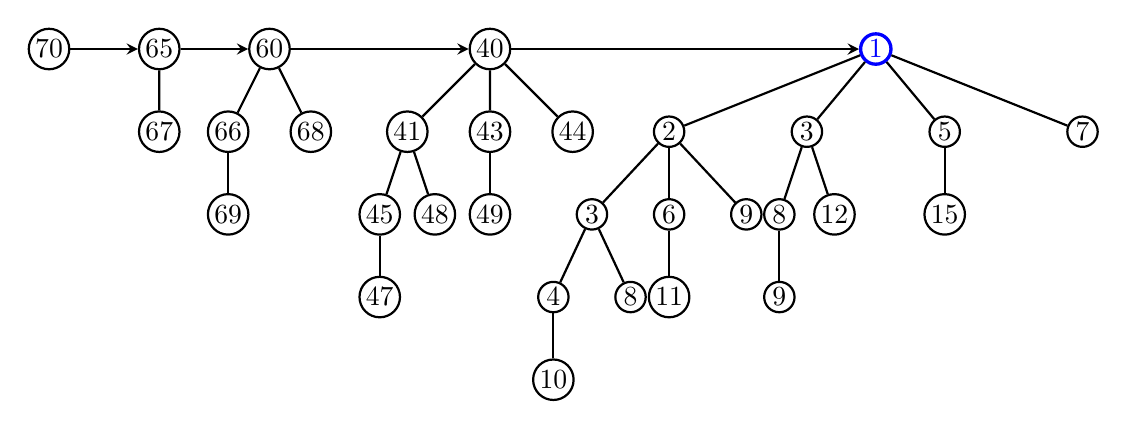
\begin{tikzpicture}
[-,thick,%
  every node/.style={shape=circle,inner sep=1pt,draw,thick},%
  scale=0.7]
\node (70) at (0,0) {$70$};
%%
\node (65) at (2,0) {$65$}
  child {node {$67$}};
%%
\node (60) at (4,0) {$60$}
  child {node {$66$}
    child {node {$69$}}
  }
  child {node {$68$}};
%%
\node (40) at (8,0) {$40$}
  child {node {$41$}
      [sibling distance=1cm]
    child {node {$45$}
      child {node {$47$}}
    }
    child {node {$48$}}
  }
  child {node {$43$}
    child {node {$49$}}
  }
  child {node {$44$}};
%%
\node[blue,very thick] (1) at (15,0) {$1$}
  [sibling distance=2.5cm]
  child {node {$2$}
    [sibling distance=1.4cm]
    child {node {$3$}
      child {node {$4$}
        child {node {$10$}}
      }
      child {node {$8$}}
    }
    child {node {$6$}
      child {node {$11$}}
    }
    child {node {$9$}}
  }
  child {node {$3$}
    [sibling distance=1cm]
    child {node {$8$}
      child {node {$9$}}
    }
    child {node {$12$}}
  }
  child {node {$5$}
    [sibling distance=1cm]
    child {node {$15$}}
  }
  child {node {$7$}};
\path
\foreach \startNode/\endNode in {70/65, 65/60, 60/40, 40/1}
{
  (\startNode) edge[->,>=stealth,thick] (\endNode)
};
\end{tikzpicture}
}
%%
%%
\subfigure[]{
\scriptsize
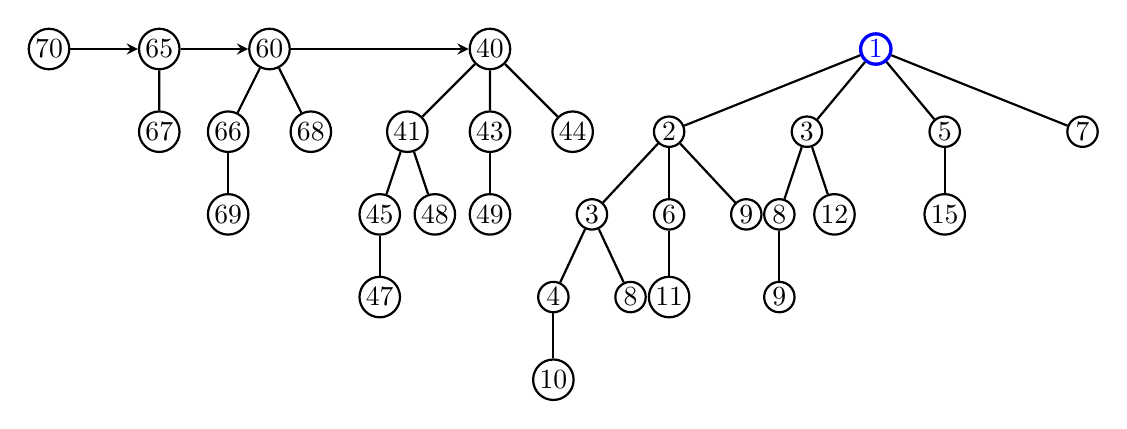
\begin{tikzpicture}
[-,thick,%
  every node/.style={shape=circle,inner sep=1pt,draw,thick},%
  scale=0.7]
\node (70) at (0,0) {$70$};
%%
\node (65) at (2,0) {$65$}
  child {node {$67$}};
%%
\node (60) at (4,0) {$60$}
  child {node {$66$}
    child {node {$69$}}
  }
  child {node {$68$}};
%%
\node (40) at (8,0) {$40$}
  child {node {$41$}
    [sibling distance=1cm]
    child {node {$45$}
      child {node {$47$}}
    }
    child {node {$48$}}
  }
  child {node {$43$}
    child {node {$49$}}
  }
  child {node {$44$}};
%%
\node[blue,very thick] at (15,0) {$1$}
  [sibling distance=2.5cm]
  child {node {$2$}
    [sibling distance=1.4cm]
    child {node {$3$}
      child {node {$4$}
        child {node {$10$}}
      }
      child {node {$8$}}
    }
    child {node {$6$}
      child {node {$11$}}
    }
    child {node {$9$}}
  }
  child {node {$3$}
    [sibling distance=1cm]
    child {node {$8$}
      child {node {$9$}}
    }
    child {node {$12$}}
  }
  child {node {$5$}
    [sibling distance=1cm]
    child {node {$15$}}
  }
  child {node {$7$}};
\path
\foreach \startNode/\endNode in {70/65, 65/60, 60/40}
{
  (\startNode) edge[->,>=stealth,thick] (\endNode)
};
\end{tikzpicture}
}
%%
%%
\subfigure[]{
\scriptsize
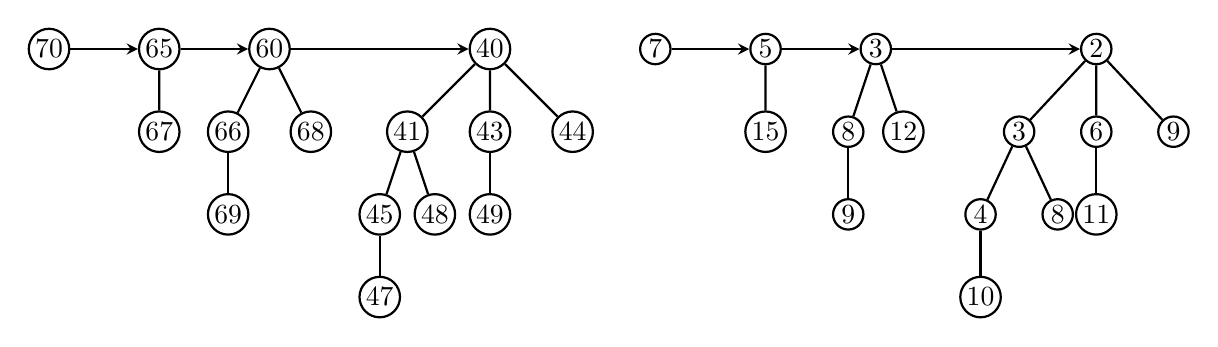
\begin{tikzpicture}
[-,thick,%
  every node/.style={shape=circle,inner sep=1pt,draw,thick},%
  scale=0.7]
\node (70) at (0,0) {$70$};
%%
\node (65) at (2,0) {$65$}
  child {node {$67$}};
%%
\node (60) at (4,0) {$60$}
  child {node {$66$}
    child {node {$69$}}
  }
  child {node {$68$}};
%%
\node (40) at (8,0) {$40$}
  child {node {$41$}
    [sibling distance=1cm]
    child {node {$45$}
      child {node {$47$}}
    }
    child {node {$48$}}
  }
  child {node {$43$}
    child {node {$49$}}
  }
  child {node {$44$}};
%%
\node (7) at (11,0) {$7$};
%%
\node (5) at (13,0) {$5$}
  child {node {$15$}};
%%
\node (3) at (15,0) {$3$}
  [sibling distance=1cm]
  child {node {$8$}
    child {node {$9$}}
  }
  child {node {$12$}};
%%
\node (2) at (19,0) {$2$}
  [sibling distance=1.4cm]
  child {node {$3$}
    child {node {$4$}
      child {node {$10$}}
    }
    child {node {$8$}}
  }
  child {node {$6$}
    child {node {$11$}}
  }
  child {node {$9$}};
\path
\foreach \startNode/\endNode in {70/65, 65/60, 60/40}
{
  (\startNode) edge[->,>=stealth,thick] (\endNode)
};
\path
\foreach \startNode/\endNode in {7/5, 5/3, 3/2}
{
  (\startNode) edge[->,>=stealth,thick] (\endNode)
};
\end{tikzpicture}
}
%%
%%
\subfigure[]{
\scriptsize
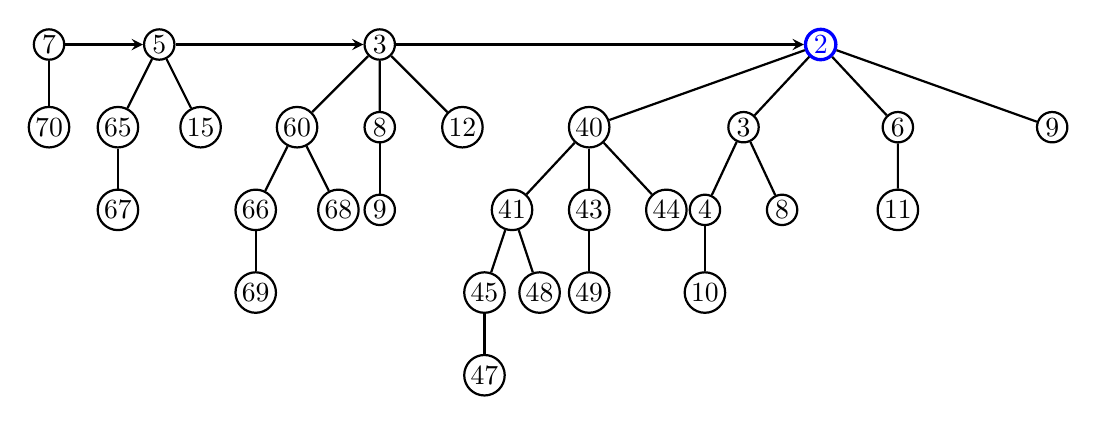
\begin{tikzpicture}
[-,thick,%
  every node/.style={shape=circle,inner sep=1pt,draw,thick},%
  scale=0.7]
\node (7) at (0,0) {$7$}
  child {node {$70$}};
%%
\node (5) at (2,0) {$5$}
  child {node {$65$}
    child {node {$67$}}
  }
  child {node {$15$}};
%%
\node (3) at (6,0) {$3$}
  child {node {$60$}
    child {node {$66$}
      child {node {$69$}}
    }
    child {node {$68$}}
  }
  child {node {$8$}
    child {node {$9$}}
  }
  child {node {$12$}};
%%
\node[blue,very thick] (2) at (14,0) {$2$}
  [sibling distance=2.8cm]
  child {node {$40$}
    [sibling distance=1.4cm]
    child {node {$41$}
      [sibling distance=1cm]
      child {node {$45$}
        child {node {$47$}}
      }
      child {node {$48$}}
    }
    child {node {$43$}
      child {node {$49$}}
    }
    child {node {$44$}}
  }
  child {node {$3$}
    [sibling distance=1.4cm]
    child {node {$4$}
      child {node {$10$}}
    }
    child {node {$8$}}
  }
  child {node {$6$}
    child {node {$11$}}
  }
  child {node {$9$}};
\path
\foreach \startNode/\endNode in {7/5, 5/3, 3/2}
{
  (\startNode) edge[->,>=stealth,thick] (\endNode)
};
\end{tikzpicture}
}
\end{figure}

\end{document}

\caption{Extracting the minimum vertex from a binomial heap.}
\label{fig:tree_data_structures:binomial_heap_extract}
\end{figure}


%%%%%%%%%%%%%%%%%%%%%%%%%%%%%%%%%%%%%%%%%%%%%%%%%%%%%%%%%%%%%%%%%%%%%%%%%%%

\section{Binary search trees}
\label{sec:tree_data_structures:binary_search_trees}

A \emph{binary search tree}\index{binary search tree}~(BST)\index{BST}
is a rooted binary tree $T = (V,E)$ having vertex weight function
$\kappa: V \to \R$. The weight of each vertex $v$ is referred to as
its key, denoted $\kappa_v$. Each vertex $v$ of $T$ satisfies the
following properties:
%%
\begin{itemize}
\item \textbf{Left subtree property.}\index{binary search tree!left subtree property}
  The left subtree of $v$ contains only vertices whose keys are at
  most $\kappa_v$. That is, if $u$ is a vertex in the left subtree of
  $v$, then $\kappa_u \leq \kappa_v$.

\item \textbf{Right subtree property.}\index{binary search tree!right subtree property}
  The right subtree of $v$ contains only vertices whose keys are at
  least $\kappa_v$. In other words, any vertex $u$ in the right
  subtree of $v$ satisfies $\kappa_v \leq \kappa_u$.

\item \textbf{Recursion property.}\index{binary search tree!recursion property}
  Both the left and right subtrees of $v$ must also be binary search
  trees.
\end{itemize}
%%
The above are collectively called the
\emph{binary search tree property}\index{binary search tree!property}.
See Figure~\ref{fig:tree_data_structures:binary_search_tree} for an
example of a binary search tree. Based on the binary search tree
property, we can use in-order\index{traversal!in-order} traversal~(see
Algorithm~\ref{alg:trees_forests:in_order_traversal}) to obtain a
listing of the vertices of a binary search tree sorted in
nondecreasing order of keys.

\begin{figure}[!htbp]
\centering
\index{binary search tree}
%%%%%%%%%%%%%%%%%%%%%%%%%%%%%%%%%%%%%%%%%%%%%%%%%%%%%%%%%%%%%%%%%%%%%%%%%%%
%% This file is part of the book
%%
%% Algorithmic Graph Theory
%% http://code.google.com/p/graph-theory-algorithms-book/
%%
%% Copyright (C) 2009--2011 Minh Van Nguyen <nguyenminh2@gmail.com>
%%
%% See the file COPYING for copying conditions.
%%%%%%%%%%%%%%%%%%%%%%%%%%%%%%%%%%%%%%%%%%%%%%%%%%%%%%%%%%%%%%%%%%%%%%%%%%%

\documentclass{article}

\usepackage{tikz}
\usetikzlibrary{external}
\usetikzlibrary{trees}
\tikzexternalize{binary-search-tree-examples}

\begin{document}

\begin{figure}
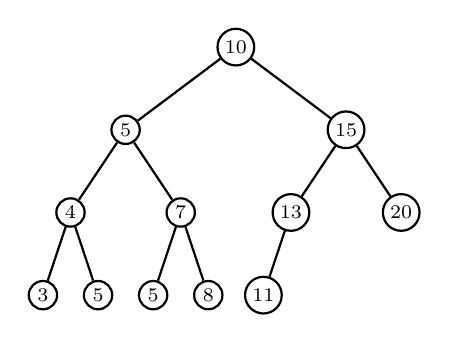
\begin{tikzpicture}
[-,thick,%
  every node/.style={shape=circle,inner sep=1.5pt,draw,thick},%
  scale=0.7]
\scriptsize
\node {$10$}
  [sibling distance=4cm]
  child {node {$5$}
    [sibling distance=2cm]
    child {node {$4$}
      [sibling distance=1cm]
      child {node {$3$}}
      child {node {$5$}}
    }
    child {node {$7$}
      [sibling distance=1cm]
      child {node {$5$}}
      child {node {$8$}}
    }
  }
  child {node {$15$}
    [sibling distance=2cm]
    child {node {$13$}
      [sibling distance=1cm]
      child {node {$11$}}
      child[missing]
    }
    child {node {$20$}}
  };
\end{tikzpicture}
\end{figure}

\end{document}

\caption{A binary search tree.}
\label{fig:tree_data_structures:binary_search_tree}
\end{figure}


%%%%%%%%%%%%%%%%%%%%%%%%%%%%%%%%%%%%%%%%%%%%%%%%%%%%%%%%%%%%%%%%%%%%%%%%%%%

\subsection{Searching}

Given a BST $T$ and a key $k$, we want to locate a vertex~(if one
exists) in $T$ whose key is $k$. The search procedure for a BST is
reminiscent of the binary\index{binary search} search algorithm
discussed in
problem~\ref{chap:graph_algorithms}.\ref{prob:graph_algorithms:binary_search}.
We begin by examining the root $v_0$ of $T$. If $\kappa_{v_0} = k$,
the search is successful. However, if $\kappa_{v_0} \neq k$ then we
have two cases to consider. In the first case, if $k < \kappa_{v_0}$
then we search the left subtree of $v_0$. The second case occurs when
$k > \kappa_{v_0}$, in which case we search the right subtree of
$v_0$. Repeat the process until a vertex $v$ in $T$ is found for which
$k = \kappa_v$ or the indicated subtree is empty. Whenever the target
key is different from the key of the vertex we are currently
considering, we move down one level of $T$. Thus if $h$ is the height
of $T$, it follows that searching $T$ takes a worst-case runtime of
$O(h)$. The above procedure is presented in pseudocode as
Algorithm~\ref{alg:tree_data_structures:binary_search_tree_locate}. Note
that if a vertex $v$ does not have a left subtree, the operation of
locating the root of $v$'s left subtree should return \texttt{NULL}. A
similar comment applies when $v$ does not have a right
subtree. Furthermore, from the structure of
Algorithm~\ref{alg:tree_data_structures:binary_search_tree_locate}, if
the input BST is empty then \texttt{NULL} is returned. See
Figure~\ref{fig:tree_data_structures:binary_search_tree_search} for an
illustration of locating vertices with given keys in a BST.

\begin{algorithm}[!htbp]
%%%%%%%%%%%%%%%%%%%%%%%%%%%%%%%%%%%%%%%%%%%%%%%%%%%%%%%%%%%%%%%%%%%%%%%%%%%
%% This file is part of the book
%%
%% Algorithmic Graph Theory
%% http://code.google.com/p/graph-theory-algorithms-book/
%%
%% Copyright (C) 2009, 2010, 2011 Minh Van Nguyen <nguyenminh2@gmail.com>
%%
%% See the file COPYING for copying conditions.
%%%%%%%%%%%%%%%%%%%%%%%%%%%%%%%%%%%%%%%%%%%%%%%%%%%%%%%%%%%%%%%%%%%%%%%%%%%

\DontPrintSemicolon
\SetAlgoNoLine
%%
%% data section
\SetKwInOut{Input}{Input}
\SetKwInOut{Output}{Output}
%%
%% input/output
\Input{A binary search tree $T$ and a target key $k$.}
\Output{A vertex in $T$ with key $k$. If no such vertex exists, return
  \texttt{NULL}.}
\BlankLine
%%
%% algorithm body
$v \assign$ root of $T$\;
\While{\rm $v \neq \texttt{NULL}$ and $k \neq \kappa_v$}{
  \eIf{$k < \kappa_v$}{
    $v \assign$ root of left subtree of $v$\;
  }{
    $v \assign$ root of right subtree of $v$\;
  }
}
\Return $v$\;

\caption{Locate a key in a binary search tree.}
\label{alg:tree_data_structures:binary_search_tree_locate}
\end{algorithm}

\begin{figure}[!htbp]
\centering
%%%%%%%%%%%%%%%%%%%%%%%%%%%%%%%%%%%%%%%%%%%%%%%%%%%%%%%%%%%%%%%%%%%%%%%%%%%
%% This file is part of the book
%%
%% Algorithmic Graph Theory
%% http://code.google.com/p/graph-theory-algorithms-book/
%%
%% Copyright (C) 2009, 2010, 2011 Minh Van Nguyen <nguyenminh2@gmail.com>
%%
%% See the file COPYING for copying conditions.
%%%%%%%%%%%%%%%%%%%%%%%%%%%%%%%%%%%%%%%%%%%%%%%%%%%%%%%%%%%%%%%%%%%%%%%%%%%

\subfigure[Vertex with key $6$: search fail.]{
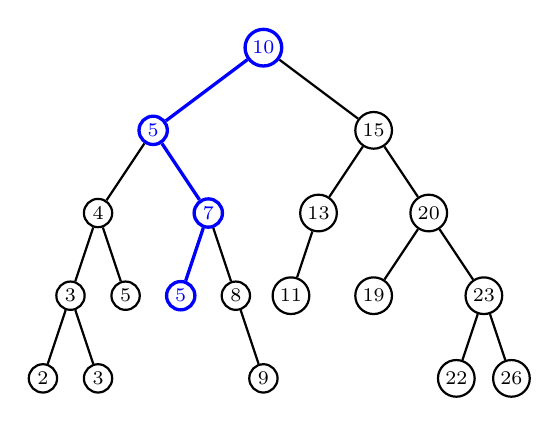
\begin{tikzpicture}
[-,thick,%
  every node/.style={shape=circle,inner sep=1.5pt,draw,thick},%
  scale=0.7]
\scriptsize
\node[blue,very thick] {$10$}
  [sibling distance=4cm]
  child[blue,very thick] {node[blue,very thick] {$5$}
    [sibling distance=2cm]
    child[black,thick] {node {$4$}
      [sibling distance=1cm]
      child {node {$3$}
        child {node {$2$}}
        child {node {$3$}}
      }
      child {node {$5$}}
    }
    child {node[blue,very thick] {$7$}
      [sibling distance=1cm]
      child {node[blue,very thick] {$5$}}
      child[black,thick] {node {$8$}
        child[missing]
        child {node {$9$}}
      }
    }
  }
  child {node {$15$}
    [sibling distance=2cm]
    child {node {$13$}
      [sibling distance=1cm]
      child {node {$11$}}
      child[missing]
    }
    child {node {$20$}
      child {node {$19$}}
      child {node {$23$}
        [sibling distance=1cm]
        child {node {$22$}}
        child {node {$26$}}
      }
    }
  };
\end{tikzpicture}
}
%%
%%
\qquad
\subfigure[Vertex with key $22$: search success.]{
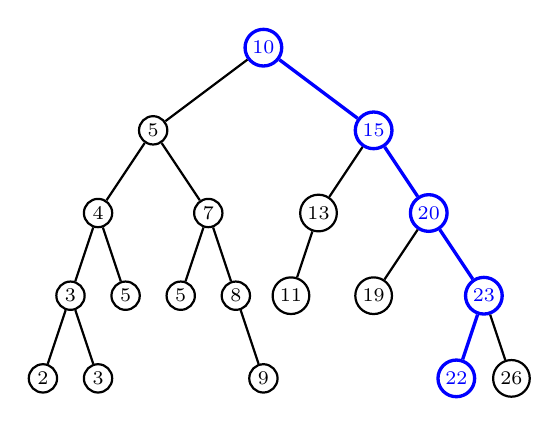
\begin{tikzpicture}
[-,thick,%
  every node/.style={shape=circle,inner sep=1.5pt,draw,thick},%
  scale=0.7]
\scriptsize
\node[blue,very thick] {$10$}
  [sibling distance=4cm]
  child {node {$5$}
    [sibling distance=2cm]
    child {node {$4$}
      [sibling distance=1cm]
      child {node {$3$}
        child {node {$2$}}
        child {node {$3$}}
      }
      child {node {$5$}}
    }
    child {node {$7$}
      [sibling distance=1cm]
      child {node {$5$}}
      child[black,thick] {node {$8$}
        child[missing]
        child {node {$9$}}
      }
    }
  }
  child[blue,very thick] {node[blue,very thick] {$15$}
    [sibling distance=2cm]
    child[black,thick] {node {$13$}
      [sibling distance=1cm]
      child {node {$11$}}
      child[missing]
    }
    child {node[blue,very thick] {$20$}
      child[black,thick] {node {$19$}}
      child {node[blue,very thick] {$23$}
        [sibling distance=1cm]
        child {node[blue,very thick] {$22$}}
        child[black,thick] {node {$26$}}
      }
    }
  };
\end{tikzpicture}
}

\caption{Finding vertices with given keys in a BST.}
\label{fig:tree_data_structures:binary_search_tree_search}
\end{figure}

\begin{figure}[!htbp]
\centering
%%%%%%%%%%%%%%%%%%%%%%%%%%%%%%%%%%%%%%%%%%%%%%%%%%%%%%%%%%%%%%%%%%%%%%%%%%%
%% This file is part of the book
%%
%% Algorithmic Graph Theory
%% http://code.google.com/p/graph-theory-algorithms-book/
%%
%% Copyright (C) 2009--2011 Minh Van Nguyen <nguyenminh2@gmail.com>
%%
%% See the file COPYING for copying conditions.
%%%%%%%%%%%%%%%%%%%%%%%%%%%%%%%%%%%%%%%%%%%%%%%%%%%%%%%%%%%%%%%%%%%%%%%%%%%

\documentclass{article}

\usepackage{subfigure}
\usepackage{tikz}
\usetikzlibrary{external}
\usetikzlibrary{trees}
\tikzexternalize{binary-search-tree-minimum-maximum}

\begin{document}

\begin{figure}
\subfigure[Minimum vertex.]{
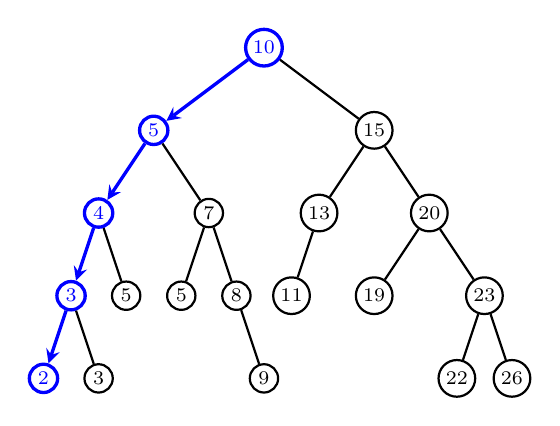
\begin{tikzpicture}
[-,thick,%
  every node/.style={shape=circle,inner sep=1.5pt,draw,thick},%
  scale=0.7]
\scriptsize
\node[blue,very thick] {$10$}
  [sibling distance=4cm]
  child[->,>=stealth,blue,very thick] {node[blue,very thick] {$5$}
    [sibling distance=2cm]
    child {node[blue,very thick] {$4$}
      [sibling distance=1cm]
      child {node[blue,very thick] {$3$}
        child {node[blue,very thick] {$2$}}
        child[-,black,thick] {node {$3$}}
      }
      child[-,black,thick] {node {$5$}}
    }
    child[-,black,thick] {node {$7$}
      [sibling distance=1cm]
      child {node {$5$}}
      child[black,thick] {node {$8$}
        child[missing]
        child {node {$9$}}
      }
    }
  }
  child {node {$15$}
    [sibling distance=2cm]
    child {node {$13$}
      [sibling distance=1cm]
      child {node {$11$}}
      child[missing]
    }
    child {node {$20$}
      child {node {$19$}}
      child {node {$23$}
        [sibling distance=1cm]
        child {node {$22$}}
        child {node {$26$}}
      }
    }
  };
\end{tikzpicture}
}
%%
%%
\qquad
\subfigure[Maximum vertex.]{
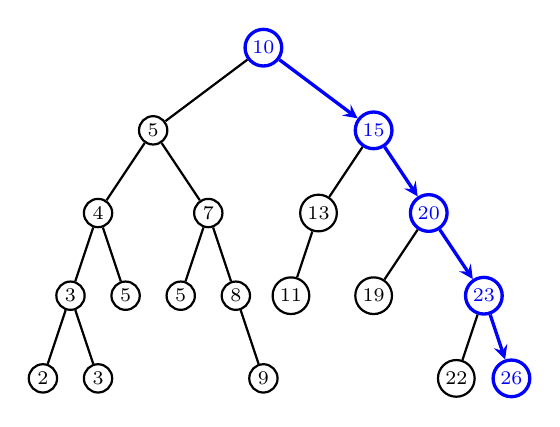
\begin{tikzpicture}
[-,thick,%
  every node/.style={shape=circle,inner sep=1.5pt,draw,thick},%
  scale=0.7]
\scriptsize
\node[blue,very thick] {$10$}
  [sibling distance=4cm]
  child {node {$5$}
    [sibling distance=2cm]
    child {node {$4$}
      [sibling distance=1cm]
      child {node {$3$}
        child {node {$2$}}
        child {node {$3$}}
      }
      child {node {$5$}}
    }
    child {node {$7$}
      [sibling distance=1cm]
      child {node {$5$}}
      child[black,thick] {node {$8$}
        child[missing]
        child {node {$9$}}
      }
    }
  }
  child[->,>=stealth,blue,very thick] {node[blue,very thick] {$15$}
    [sibling distance=2cm]
    child[-,black,thick] {node {$13$}
      [sibling distance=1cm]
      child {node {$11$}}
      child[missing]
    }
    child {node[blue,very thick] {$20$}
      child[-,black,thick] {node {$19$}}
      child {node[blue,very thick] {$23$}
        [sibling distance=1cm]
        child[-,black,thick] {node {$22$}}
        child {node[blue,very thick] {$26$}}
      }
    }
  };
\end{tikzpicture}
}
\end{figure}

\end{document}

\caption{Locating minimum and maximum vertices in a BST.}
\label{fig:tree_data_structures:binary_search_tree_minimum_maximum}
\end{figure}

\begin{figure}[!htbp]
\centering
\input{image/tree-data-structures/binary-search-tree-successor-predecessor.tex}
\caption{Searching for successor and predecessor.}
\label{fig:tree_data_structures:binary_search_tree_successor_predecessor}
\end{figure}

From the binary search tree property, deduce that a vertex of a BST
$T$ with minimum key can be found by starting from the root of $T$ and
repeatedly traversing left subtrees. When we have reached the
left-most vertex $v$ of $T$, querying for the left subtree of $v$
should return \texttt{NULL}. At this point, we conclude that $v$ is a
vertex with minimum key. Each query for the left subtree moves us one
level down $T$, resulting in a worst-case runtime of $O(h)$ with $h$
being the height of $T$. See
Algorithm~\ref{alg:tree_data_structures:binary_search_tree_minimum_key}
for pseudocode of the procedure.

The procedure for finding a vertex with maximum key is analogous to
that for finding one with minimum key. Starting from the root of $T$,
we repeatedly traverse right subtrees until we encounter the
right-most vertex, which by the binary search tree property has
maximum key. This procedure has the same worst-case runtime of $O(h)$.
Figure~\ref{fig:tree_data_structures:binary_search_tree_minimum_maximum}
illustrates the process of locating the minimum and maximum vertices
of a BST.

\begin{algorithm}[!htbp]
%%%%%%%%%%%%%%%%%%%%%%%%%%%%%%%%%%%%%%%%%%%%%%%%%%%%%%%%%%%%%%%%%%%%%%%%%%%
%% This file is part of the book
%%
%% Algorithmic Graph Theory
%% http://code.google.com/p/graph-theory-algorithms-book/
%%
%% Copyright (C) 2009, 2010, 2011 Minh Van Nguyen <nguyenminh2@gmail.com>
%%
%% See the file COPYING for copying conditions.
%%%%%%%%%%%%%%%%%%%%%%%%%%%%%%%%%%%%%%%%%%%%%%%%%%%%%%%%%%%%%%%%%%%%%%%%%%%

\DontPrintSemicolon
\SetAlgoNoLine
%%
%% data section
\SetKwInOut{Input}{Input}
\SetKwInOut{Output}{Output}
%%
%% input/output
\Input{A nonempty binary search tree $T$.}
\Output{A vertex of $T$ with minimum key.}
\BlankLine
%%
%% algorithm body
$v \assign$ root of $T$\;
\While{\rm $v$ has a left subtree}{
  $v \assign$ root of left subtree of $v$\;
}
\Return $v$\;

\caption{Finding a vertex with minimum key in a BST.}
\label{alg:tree_data_structures:binary_search_tree_minimum_key}
\end{algorithm}

Corresponding to the notions of left- and right-children, we can also
define successors and predecessors as follows. Suppose $v$ is not a
maximum vertex of a nonempty BST $T$. The \emph{successor} of $v$ is a
vertex in $T$ distinct from $v$ with the smallest key greater than or
equal to $\kappa_v$. Similarly, for a vertex $v$ that is not a minimum
vertex of $T$, the \emph{predecessor} of $v$ is a vertex in $T$
distinct from $v$ with the greatest key less than or equal to
$\kappa_v$. The notions of successors and predecessors are concerned
with relative key order, not a vertex's position within the
hierarchical structure of a BST. For instance, from
Figure~\ref{fig:tree_data_structures:binary_search_tree} we see that
the successor of the vertex $u$ with key $8$ is the vertex $v$ with
key $10$, i.e. the root, even though $v$ is an ancestor of $u$. The
predecessor of the vertex $a$ with key $4$ is the vertex $b$ with key
$3$, i.e. the minimum vertex, even though $b$ is a descendant of $a$.

We now describe a method to systematically locate the successor of a
given vertex. Let $T$ be a nonempty BST and $v \in V(T)$ not a maximum
vertex of $T$. If $v$ has a right subtree, then we find a minimum
vertex of $v$'s right subtree. In case $v$ does not have a right
subtree, we backtrack up one level to $v$'s parent
$u = \parent(v)$. If $v$ is the root of the right subtree of $u$, we
backtrack up one level again to $u$'s parent, making the assignments
$v \assign u$ and $u \assign \parent(u)$. Otherwise we return $v$'s
parent. Repeat the above backtracking procedure until the required
successor is found. Our discussion is summarized in
Algorithm~\ref{alg:tree_data_structures:binary_search_tree_successors}.
Each time we backtrack to a vertex's parent, we move up one
level, hence the worst-case runtime of
Algorithm~\ref{alg:tree_data_structures:binary_search_tree_successors}
is $O(h)$ with $h$ being the height of $T$. The procedure for finding
predecessors is similar. Refer to
Figure~\ref{fig:tree_data_structures:binary_search_tree_successor_predecessor}
for an illustration of locating successors and predecessors.

\begin{algorithm}[!htbp]
%%%%%%%%%%%%%%%%%%%%%%%%%%%%%%%%%%%%%%%%%%%%%%%%%%%%%%%%%%%%%%%%%%%%%%%%%%%
%% This file is part of the book
%%
%% Algorithmic Graph Theory
%% http://code.google.com/p/graph-theory-algorithms-book/
%%
%% Copyright (C) 2009, 2010, 2011 Minh Van Nguyen <nguyenminh2@gmail.com>
%%
%% See the file COPYING for copying conditions.
%%%%%%%%%%%%%%%%%%%%%%%%%%%%%%%%%%%%%%%%%%%%%%%%%%%%%%%%%%%%%%%%%%%%%%%%%%%

\DontPrintSemicolon
\SetAlgoNoLine
%%
%% data section
\SetKwInOut{Input}{Input}
\SetKwInOut{Output}{Output}
%%
%% input/output
\Input{A nonempty binary search tree $T$ and a vertex $v$ that is not
  a maximum of $T$.}
\Output{The successor of $v$.}
\BlankLine
%%
%% algorithm body
\If{\rm $\rightChild[v] \neq \texttt{NULL}$}{
  \Return minimum vertex of $v$'s right subtree as per Algorithm~\ref{alg:tree_data_structures:binary_search_tree_minimum_key}\;
}
$u \assign \parent(v)$\;
\While{\rm $u \neq \texttt{NULL}$ and $v = \rightChild[u]$}{
  $v \assign u$\;
  $u \assign \parent(u)$\;
}
\Return $u$\;

\caption{Finding successors in a binary search tree.}
\label{alg:tree_data_structures:binary_search_tree_successors}
\end{algorithm}


%%%%%%%%%%%%%%%%%%%%%%%%%%%%%%%%%%%%%%%%%%%%%%%%%%%%%%%%%%%%%%%%%%%%%%%%%%%

\subsection{Insertion}

Inserting a vertex $v$ into a BST $T$ is rather straightforward. If
$T$ is empty, we let $v$ be the root of $T$. Otherwise $T$ has at
least one vertex. In that case, we need to locate a vertex in $T$ that
can act as a parent and ``adopt'' $v$ as a child. To find a candidate
parent, let $u$ be the root of $T$. If $\kappa_v < \kappa_u$ then we
assign the root of the left subtree of $u$ to $u$ itself. Otherwise we
assign the root of the right subtree of $u$ to $u$. We then carry on
the above key comparison process until the operation of locating the
root of a left or right subtree returns \texttt{NULL}. At this point,
a candidate parent for $v$ is the last non-\texttt{NULL} value of
$u$. If $\kappa_v < \kappa_u$ then we let $v$ be $u$'s
left-child. Otherwise $v$ is the right-child of $u$. After each key
comparison, we move down at most one level so that in the worst-case
inserting a vertex in $T$ takes $O(h)$ time, where $h$ is the height
of $T$.
Algorithm~\ref{alg:tree_data_structures:binary_search_tree_insert}
presents pseudocode of our discussion and
Figure~\ref{fig:tree_data_structures:binary_search_tree_insert}
illustrates how to insert a vertex into a BST.

\begin{algorithm}[!htbp]
%%%%%%%%%%%%%%%%%%%%%%%%%%%%%%%%%%%%%%%%%%%%%%%%%%%%%%%%%%%%%%%%%%%%%%%%%%%
%% This file is part of the book
%%
%% Algorithmic Graph Theory
%% http://code.google.com/p/graph-theory-algorithms-book/
%%
%% Copyright (C) 2009, 2010, 2011 Minh Van Nguyen <nguyenminh2@gmail.com>
%%
%% See the file COPYING for copying conditions.
%%%%%%%%%%%%%%%%%%%%%%%%%%%%%%%%%%%%%%%%%%%%%%%%%%%%%%%%%%%%%%%%%%%%%%%%%%%

\DontPrintSemicolon
\SetAlgoNoLine
%%
%% data section
\SetKwData{NULL}{\footnotesize{NULL}}
%%
%% input
\KwIn{A binary search tree $T$ and a vertex $x$ to be inserted into $T$.}
%%
%% output
\KwOut{The same BST $T$ but augmeneted with $x$.}
\BlankLine
%%
%% algorithm body
$u \assign \NULL$\;
$v \assign$ root of $T$\;
\While{$v \neq \NULL$}{
  $u \assign v$\;
  \If{$\kappa_x < \kappa_v$}{
    $v \assign \leftChild[v]$\;
  }
  \Else{
    $v \assign \rightChild[v]$\;
  }
}
$\parent[x] \assign u$\;
\If{$u = \NULL$}{
  $\rootElem[T] \assign x$\;
}
\Else{
  \If{$\kappa_x < \kappa_u$}{
    $\leftChild[u] \assign x$\;
  }
  \Else{
    $\rightChild[u] \assign x$\;
  }
}

\caption{Inserting a vertex into a binary search tree.}
\label{alg:tree_data_structures:binary_search_tree_insert}
\end{algorithm}

\begin{figure}[!htbp]
\centering
%%%%%%%%%%%%%%%%%%%%%%%%%%%%%%%%%%%%%%%%%%%%%%%%%%%%%%%%%%%%%%%%%%%%%%%%%%%
%% This file is part of the book
%%
%% Algorithmic Graph Theory
%% http://code.google.com/p/graph-theory-algorithms-book/
%%
%% Copyright (C) 2009--2011 Minh Van Nguyen <nguyenminh2@gmail.com>
%%
%% See the file COPYING for copying conditions.
%%%%%%%%%%%%%%%%%%%%%%%%%%%%%%%%%%%%%%%%%%%%%%%%%%%%%%%%%%%%%%%%%%%%%%%%%%%

\documentclass{article}

\usepackage{subfigure}
\usepackage{tikz}
\usetikzlibrary{external}
\usetikzlibrary{trees}
\tikzexternalize{binary-search-tree-insert}

\begin{document}

\begin{figure}
\subfigure[]{
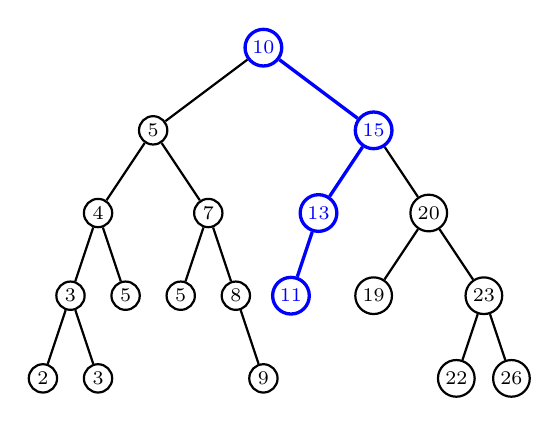
\begin{tikzpicture}
[-,thick,%
  every node/.style={shape=circle,inner sep=1.5pt,draw,thick},%
  scale=0.7]
\scriptsize
\node[blue,very thick] {$10$}
  [sibling distance=4cm]
  child {node {$5$}
    [sibling distance=2cm]
    child {node {$4$}
      [sibling distance=1cm]
      child {node {$3$}
        child {node {$2$}}
        child {node {$3$}}
      }
      child {node {$5$}}
    }
    child {node {$7$}
      [sibling distance=1cm]
      child {node {$5$}}
      child {node {$8$}
        child[missing]
        child {node {$9$}}
      }
    }
  }
  child[blue,very thick] {node[blue,very thick] {$15$}
    [sibling distance=2cm]
    child {node[blue,very thick] {$13$}
      [sibling distance=1cm]
      child {node[blue,very thick] {$11$}}
      child[missing]
    }
    child[black,thick] {node {$20$}
      child {node {$19$}}
      child {node {$23$}
        [sibling distance=1cm]
        child {node {$22$}}
        child {node {$26$}}
      }
    }
  };
\end{tikzpicture}
}
%%
%%
\qquad
\subfigure[]{
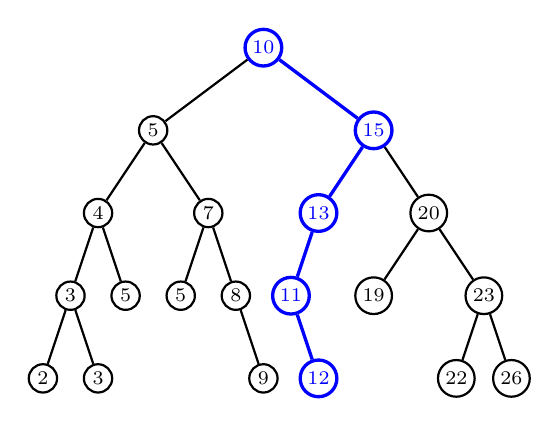
\begin{tikzpicture}
[-,thick,%
  every node/.style={shape=circle,inner sep=1.5pt,draw,thick},%
  scale=0.7]
\scriptsize
\node[blue,very thick] {$10$}
  [sibling distance=4cm]
  child {node {$5$}
    [sibling distance=2cm]
    child {node {$4$}
      [sibling distance=1cm]
      child {node {$3$}
        child {node {$2$}}
        child {node {$3$}}
      }
      child {node {$5$}}
    }
    child {node {$7$}
      [sibling distance=1cm]
      child {node {$5$}}
      child[black,thick] {node {$8$}
        child[missing]
        child {node {$9$}}
      }
    }
  }
  child[blue,very thick] {node[blue,very thick] {$15$}
    [sibling distance=2cm]
    child {node[blue,very thick] {$13$}
      [sibling distance=1cm]
      child {node[blue,very thick] {$11$}
        child[missing]
        child {node[blue,very thick] {$12$}}
      }
      child[missing]
    }
    child[black,thick] {node {$20$}
      child {node {$19$}}
      child {node {$23$}
        [sibling distance=1cm]
        child {node {$22$}}
        child {node {$26$}}
      }
    }
  };
\end{tikzpicture}
}
\end{figure}

\end{document}

\caption{Inserting into a binary search tree.}
\label{fig:tree_data_structures:binary_search_tree_insert}
\end{figure}


%%%%%%%%%%%%%%%%%%%%%%%%%%%%%%%%%%%%%%%%%%%%%%%%%%%%%%%%%%%%%%%%%%%%%%%%%%%

\subsection{Deletion}

\begin{algorithm}[!htbp]
%%%%%%%%%%%%%%%%%%%%%%%%%%%%%%%%%%%%%%%%%%%%%%%%%%%%%%%%%%%%%%%%%%%%%%%%%%%
%% This file is part of the book
%%
%% Algorithmic Graph Theory
%% http://code.google.com/p/graph-theory-algorithms-book/
%%
%% Copyright (C) 2009, 2010, 2011 Minh Van Nguyen <nguyenminh2@gmail.com>
%%
%% See the file COPYING for copying conditions.
%%%%%%%%%%%%%%%%%%%%%%%%%%%%%%%%%%%%%%%%%%%%%%%%%%%%%%%%%%%%%%%%%%%%%%%%%%%

\DontPrintSemicolon
\SetAlgoNoLine
%%
%% data section
\SetKwData{NULL}{\footnotesize{NULL}}
%%
%% input
\KwIn{A nonempty binary search tree $T$ and a vertex $x \in V(T)$ to
  be removed from $T$.}
%%
%% output
\KwOut{The same BST $T$ but without $x$.}
\BlankLine
%%
%% algorithm body
$u \assign \NULL$\;
$v \assign \NULL$\;
\If{\rm $\leftChild[x] \neq \NULL$ or $\rightChild[x] \neq \NULL$}{
  $v \assign x$\;
}
\Else{
  $v \assign$ successor of $x$\;
}
\If{$\leftChild[v] \neq \NULL$}{
  $u \assign \leftChild[v]$\;
}
\Else{
  $u \assign \rightChild[v]$\;
}
\If{$u \neq \NULL$}{
  $\parent[u] \assign \parent[v]$\;
}
\If{$\parent[v] = \NULL$}{
  $\rootElem[T] \assign u$\;
}
\Else{
  \If{$v = \leftChild[\parent[v]]$}{
    $\leftChild[\parent[v]] \assign u$\;
  }
  \Else{
    $\rightChild[\parent[v]] \assign u$\;
  }
}
\If{$v \neq x$}{
  $\kappa_x \assign \kappa_v$\;
  copy $v$'s auxilary data into $x$\;
}

\caption{Deleting a vertex from a binary search tree.}
\label{alg:tree_data_structures:binary_search_tree_delete}
\end{algorithm}

\noindent
Whereas insertion into a BST is straightforward, removing a vertex
requires much more work. Let $T$ be a nonempty binary search tree and
suppose we want to remove $v \in V(T)$ from $T$. Having located the
position that $v$ occupies within $T$, we need to consider three
separate cases: (1)~$v$ is a leaf; (2)~$v$ has one child; (3)~$v$ has
two children.
%%
\begin{enumerate}
\item If $v$ is a leaf, we simply remove $v$ from $T$ and the
  procedure is complete. The resulting tree without $v$ satisfies the
  binary search tree property.

\item Suppose $v$ has the single child $u$. Removing $v$ would
  disconnect $T$, a situation that can be prevented by splicing out
  $u$ and letting $u$ occupy the position previously held by $v$. The
  resulting tree with $v$ removed as described satisfies the binary
  search tree property.

\item Finally suppose $v$ has two children and let $s$ and $p$ be the
  successor and predecessor of $v$, respectively. It can be shown that
  $s$ has no left-child and $p$ has no right-child. We can choose to
  either splice out $s$ or $p$. Say we choose to splice out $s$. Then
  we remove $v$ and let $s$ hold the position previously occupied by
  $v$. The resulting tree with $v$ thus removed satisfies the binary
  search tree property.
\end{enumerate}
%%
The above procedure is summarized in
Algorithm~\ref{alg:tree_data_structures:binary_search_tree_delete},
which is adapted from~\cite[p.262]{CormenEtAl2001}.
Figure~\ref{fig:tree_data_structures:binary_search_tree_delete}
illustrates the various cases to be considered when removing a vertex
from a BST. Note that in
Algorithm~\ref{alg:tree_data_structures:binary_search_tree_delete},
the process of finding the successor dominates the runtime of the
entire algorithm. Other operations in the algorithm take at most
constant time. Therefore deleting a vertex from a binary search tree
can be accomplished in worst-case $O(h)$ time, where $h$ is the height
of the BST under consideration.

\begin{figure}[!htbp]
\centering
%%%%%%%%%%%%%%%%%%%%%%%%%%%%%%%%%%%%%%%%%%%%%%%%%%%%%%%%%%%%%%%%%%%%%%%%%%%
%% This file is part of the book
%%
%% Algorithmic Graph Theory
%% http://code.google.com/p/graph-theory-algorithms-book/
%%
%% Copyright (C) 2009, 2010, 2011 Minh Van Nguyen <nguyenminh2@gmail.com>
%%
%% See the file COPYING for copying conditions.
%%%%%%%%%%%%%%%%%%%%%%%%%%%%%%%%%%%%%%%%%%%%%%%%%%%%%%%%%%%%%%%%%%%%%%%%%%%

\documentclass{article}

\usepackage{subfigure}
\usepackage{tikz}
\usetikzlibrary{external}
\usetikzlibrary{trees}
\tikzexternalize{binary-search-tree-delete}

\begin{document}

\begin{figure}
\subfigure[Target vertex $9$ is a leaf.]{
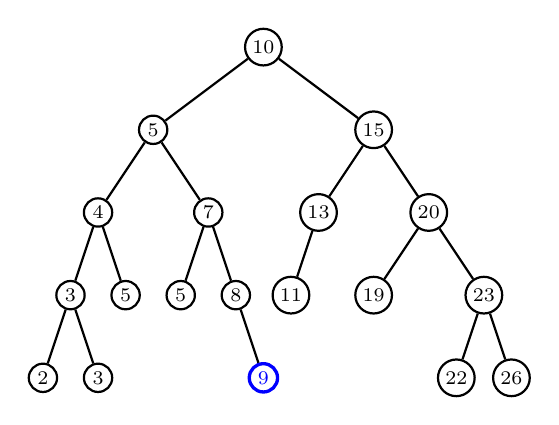
\begin{tikzpicture}
[-,thick,%
  every node/.style={shape=circle,inner sep=1.5pt,draw,thick},%
  scale=0.7]
\scriptsize
\node {$10$}
  [sibling distance=4cm]
  child {node {$5$}
    [sibling distance=2cm]
    child {node {$4$}
      [sibling distance=1cm]
      child {node {$3$}
        child {node {$2$}}
        child {node {$3$}}
      }
      child {node {$5$}}
    }
    child {node {$7$}
      [sibling distance=1cm]
      child {node {$5$}}
      child {node {$8$}
        child[missing]
        child {node[blue,very thick] {$9$}}
      }
    }
  }
  child {node {$15$}
    [sibling distance=2cm]
    child {node {$13$}
      [sibling distance=1cm]
      child {node {$11$}}
      child[missing]
    }
    child {node {$20$}
      child {node {$19$}}
      child {node {$23$}
        [sibling distance=1cm]
        child {node {$22$}}
        child {node {$26$}}
      }
    }
  };
\end{tikzpicture}
}
%%
%%
\qquad
\subfigure[Leaf deleted.]{
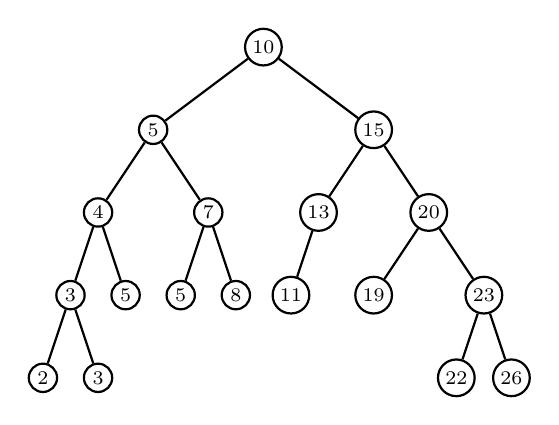
\begin{tikzpicture}
[-,thick,%
  every node/.style={shape=circle,inner sep=1.5pt,draw,thick},%
  scale=0.7]
\scriptsize
\node {$10$}
  [sibling distance=4cm]
  child {node {$5$}
    [sibling distance=2cm]
    child {node {$4$}
      [sibling distance=1cm]
      child {node {$3$}
        child {node {$2$}}
        child {node {$3$}}
      }
      child {node {$5$}}
    }
    child {node {$7$}
      [sibling distance=1cm]
      child {node {$5$}}
      child {node {$8$}}
    }
  }
  child {node {$15$}
    [sibling distance=2cm]
    child {node {$13$}
      [sibling distance=1cm]
      child {node {$11$}}
      child[missing]
    }
    child {node {$20$}
      child {node {$19$}}
      child {node {$23$}
        [sibling distance=1cm]
        child {node {$22$}}
        child {node {$26$}}
      }
    }
  };
\end{tikzpicture}
}
%%
%%
\subfigure[Target vertex $13$ has one child.]{
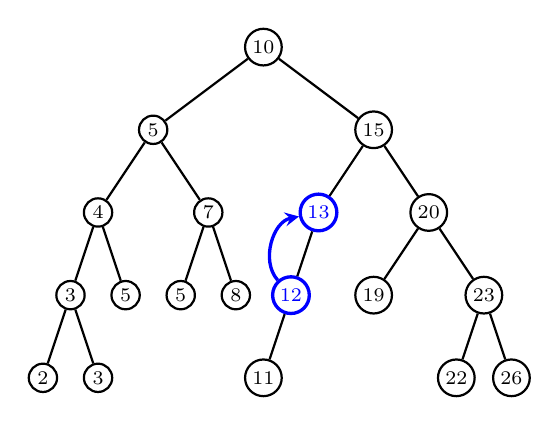
\begin{tikzpicture}
[-,thick,%
  every node/.style={shape=circle,inner sep=1.5pt,draw,thick},%
  scale=0.7]
\scriptsize
\node {$10$}
  [sibling distance=4cm]
  child {node {$5$}
    [sibling distance=2cm]
    child {node {$4$}
      [sibling distance=1cm]
      child {node {$3$}
        child {node {$2$}}
        child {node {$3$}}
      }
      child {node {$5$}}
    }
    child {node {$7$}
      [sibling distance=1cm]
      child {node {$5$}}
      child {node {$8$}}
    }
  }
  child {node {$15$}
    [sibling distance=2cm]
    child {node[blue,very thick] (13) {$13$}
      [sibling distance=1cm]
      child {node[blue,very thick] (12) {$12$}
        child {node {$11$}}
        child[missing]
      }
      child[missing]
    }
    child {node {$20$}
      child {node {$19$}}
      child {node {$23$}
        [sibling distance=1cm]
        child {node {$22$}}
        child {node {$26$}}
      }
    }
  };
\path
(12) edge[->,>=stealth,blue,very thick,bend left=60] (13);
\end{tikzpicture}
}
%%
%%
\qquad
\subfigure[Vertex deleted.]{
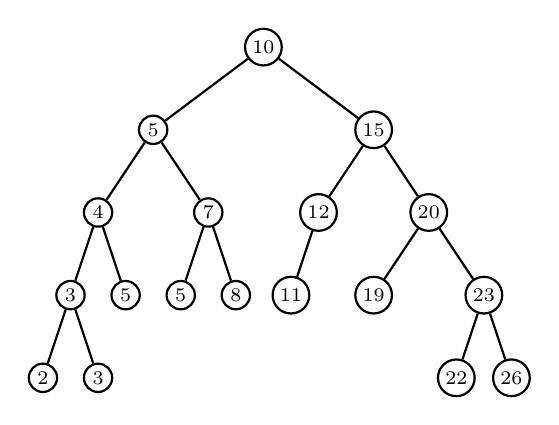
\begin{tikzpicture}
[-,thick,%
  every node/.style={shape=circle,inner sep=1.5pt,draw,thick},%
  scale=0.7]
\scriptsize
\node {$10$}
  [sibling distance=4cm]
  child {node {$5$}
    [sibling distance=2cm]
    child {node {$4$}
      [sibling distance=1cm]
      child {node {$3$}
        child {node {$2$}}
        child {node {$3$}}
      }
      child {node {$5$}}
    }
    child {node {$7$}
      [sibling distance=1cm]
      child {node {$5$}}
      child {node {$8$}}
    }
  }
  child {node {$15$}
    [sibling distance=2cm]
    child {node {$12$}
      [sibling distance=1cm]
      child {node {$11$}}
      child[missing]
    }
    child {node {$20$}
      child {node {$19$}}
      child {node {$23$}
        [sibling distance=1cm]
        child {node {$22$}}
        child {node {$26$}}
      }
    }
  };
\end{tikzpicture}
}
%%
%%
\subfigure[Target vertex $15$ has two children.]{
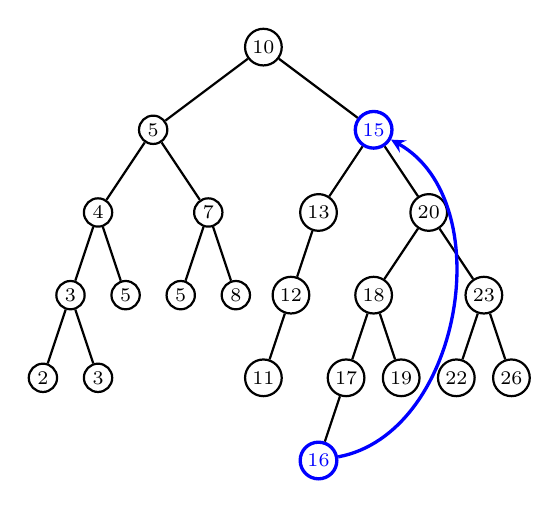
\begin{tikzpicture}
[-,thick,%
  every node/.style={shape=circle,inner sep=1.5pt,draw,thick},%
  scale=0.7]
\scriptsize
\node {$10$}
  [sibling distance=4cm]
  child {node {$5$}
    [sibling distance=2cm]
    child {node {$4$}
      [sibling distance=1cm]
      child {node {$3$}
        child {node {$2$}}
        child {node {$3$}}
      }
      child {node {$5$}}
    }
    child {node {$7$}
      [sibling distance=1cm]
      child {node {$5$}}
      child {node {$8$}}
    }
  }
  child {node[blue,very thick] (15) {$15$}
    [sibling distance=2cm]
    child {node {$13$}
      [sibling distance=1cm]
      child {node {$12$}
        child {node {$11$}}
        child[missing]
      }
      child[missing]
    }
    child {node {$20$}
      child {node {$18$}
        [sibling distance=1cm]
        child {node {$17$}
          child {node[blue,very thick] (16) {$16$}}
          child[missing]
        }
        child {node {$19$}}
      }
      child {node {$23$}
        [sibling distance=1cm]
        child {node {$22$}}
        child {node {$26$}}
      }
    }
  };
\path
(16) edge[->,>=stealth,blue,very thick,bend right=70] (15);
\end{tikzpicture}
}
%%
%%
\qquad
\subfigure[Vertex deleted.]{
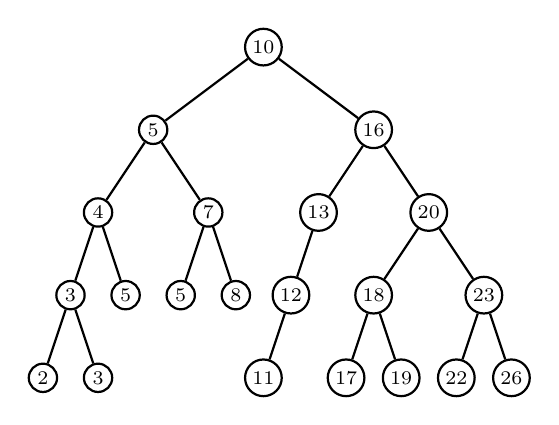
\begin{tikzpicture}
[-,thick,%
  every node/.style={shape=circle,inner sep=1.5pt,draw,thick},%
  scale=0.7]
\scriptsize
\node {$10$}
  [sibling distance=4cm]
  child {node {$5$}
    [sibling distance=2cm]
    child {node {$4$}
      [sibling distance=1cm]
      child {node {$3$}
        child {node {$2$}}
        child {node {$3$}}
      }
      child {node {$5$}}
    }
    child {node {$7$}
      [sibling distance=1cm]
      child {node {$5$}}
      child {node {$8$}}
    }
  }
  child {node {$16$}
    [sibling distance=2cm]
    child {node {$13$}
      [sibling distance=1cm]
      child {node {$12$}
        child {node {$11$}}
        child[missing]
      }
      child[missing]
    }
    child {node {$20$}
      child {node {$18$}
        [sibling distance=1cm]
        child {node {$17$}}
        child {node {$19$}}
      }
      child {node {$23$}
        [sibling distance=1cm]
        child {node {$22$}}
        child {node {$26$}}
      }
    }
  };
\end{tikzpicture}
}
\end{figure}

\end{document}

\caption{Deleting a vertex from a binary search tree.}
\label{fig:tree_data_structures:binary_search_tree_delete}
\end{figure}

\begin{figure}[!htbp]
\centering
\index{binary search tree}
%%%%%%%%%%%%%%%%%%%%%%%%%%%%%%%%%%%%%%%%%%%%%%%%%%%%%%%%%%%%%%%%%%%%%%%%%%%
%% This file is part of the book
%%
%% Algorithmic Graph Theory
%% http://code.google.com/p/graph-theory-algorithms-book/
%%
%% Copyright (C) 2009, 2010, 2011 Minh Van Nguyen <nguyenminh2@gmail.com>
%%
%% See the file COPYING for copying conditions.
%%%%%%%%%%%%%%%%%%%%%%%%%%%%%%%%%%%%%%%%%%%%%%%%%%%%%%%%%%%%%%%%%%%%%%%%%%%

\subfigure[]{
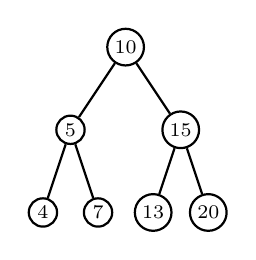
\begin{tikzpicture}
[-,thick,%
  every node/.style={shape=circle,inner sep=1.5pt,draw,thick},%
  scale=0.7]
\scriptsize
\node {$10$}
  [sibling distance=2cm]
  child {node {$5$}
    [sibling distance=1cm]
    child {node {$4$}}
    child {node {$7$}}
  }
  child {node {$15$}
    [sibling distance=1cm]
    child {node {$13$}}
    child {node {$20$}}
  };
\end{tikzpicture}
}
%%
%%
\qquad
\subfigure[]{
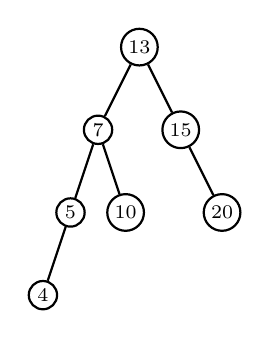
\begin{tikzpicture}
[-,thick,%
  every node/.style={shape=circle,inner sep=1.5pt,draw,thick},%
  scale=0.7]
\scriptsize
\node {$13$}
  child {node {$7$}
    [sibling distance=1cm]
    child {node {$5$}
      child {node {$4$}}
      child[missing]
    }
    child {node {$10$}}
  }
  child {node {$15$}
    child[missing]
    child {node {$20$}}
  };
\end{tikzpicture}
}
%%
%%
\qquad
\subfigure[]{
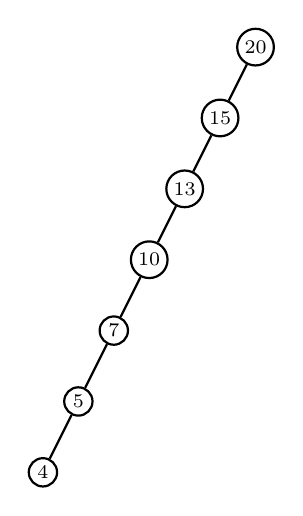
\begin{tikzpicture}
[-,thick,%
  every node/.style={shape=circle,inner sep=1.5pt,draw,thick},%
  scale=0.6]
\scriptsize
\node {$20$}
  child {node {$15$}
    child {node {$13$}
      child {node {$10$}
        child {node {$7$}
          child {node {$5$}
            child {node {$4$}}
            child[missing]
          }
          child[missing]
        }
        child[missing]
      }
      child[missing]
    }
    child[missing]
  }
  child[missing];
\end{tikzpicture}
}
%%
%%
\qquad
\subfigure[]{
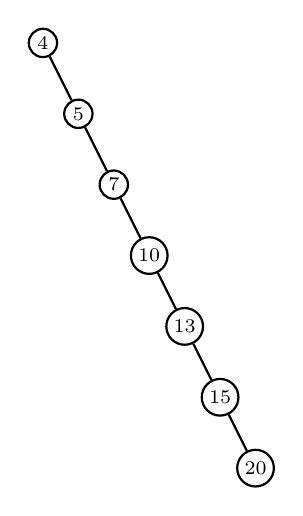
\begin{tikzpicture}
[-,thick,%
  every node/.style={shape=circle,inner sep=1.5pt,draw,thick},%
  scale=0.6]
\scriptsize
\node {$4$}
  child[missing]
  child{node {$5$}
    child[missing]
    child {node {$7$}
      child[missing]
      child {node {$10$}
        child[missing]
        child {node {$13$}
          child[missing]
          child {node {$15$}
            child[missing]
            child {node {$20$}}
          }
        }
      }
    }
  };
\end{tikzpicture}
}

\caption{Different structural representations of a BST.}
\label{fig:tree_data_structures:BST_different_structural_representations}
\end{figure}


%%%%%%%%%%%%%%%%%%%%%%%%%%%%%%%%%%%%%%%%%%%%%%%%%%%%%%%%%%%%%%%%%%%%%%%%%%%

\section{AVL trees}
\index{AVL tree}

To motivate the need for AVL\index{AVL tree} trees, note the lack of a
structural property for binary\index{binary search tree} search trees
similar to the structural\index{binary heap!heap-structure property}
property for binary\index{binary heap} heaps. Unlike binary heaps, a
BST is not required to have as small a height as possible. As a
consequence, any given nonempty collection
$C = \{v_0, v_1, \dots, v_k\}$ of weighted vertices can be represented
by various BSTs with different heights; see
Figure~\ref{fig:tree_data_structures:BST_different_structural_representations}.
Some BST representations of $C$ have heights smaller than other BST
representations of $C$. Those BST representations with smaller heights
can result in reduced time for basic operations such as search,
insertion, and deletion and out-perform BST representations having
larger heights. To achieve logarithmic or near-logarithmic time
complexity for basic operations, it is desirable to maintain a BST
with as small a height as possible.

Adel'son-Vel'ski\u{\i}\index{Adel'son-Vel'ski\u{\i}, G. M.} and
Landis\index{Landis, E. M.}~\cite{AdelsonVelskiiLandis1962}
introduced in~1962 a criterion for constructing and maintaining binary
search trees having logarithmic heights. Recall that the height of a
tree is the maximum depth of the tree. Then the
Adel'son-Vel'ski\u{\i}-Landis criterion can be expressed as follows.

\begin{definition}
\textbf{Height-balance property.}\index{AVL tree!height-balance property}
Let $T$ be a binary tree and suppose $v$ is an internal vertex of
$T$. Let $h_\ell$ be the height of the left subtree of $v$ and let
$h_r$ be the height of $v$'s right subtree. Then $T$ is said to be
\emph{height-balanced} if $|h_\ell - h_r| \leq 1$.
\end{definition}

Binary trees having the height-balance property are called
AVL\index{AVL tree} trees. The structure of such trees is such that
given any internal vertex $v$ of an AVL tree, the heights of the left
and right subtrees of $v$ differ by at most $1$.
Complete\index{binary tree!complete} binary trees are trivial examples
of AVL trees, as are nearly\index{binary tree!nearly complete}
complete binary trees. A less trivial example of AVL trees are what is
known as \emph{Fibonacci trees}\index{Fibonacci!tree}, so named
because the construction of Fibonacci trees bears some resemblance to
how Fibonacci numbers\index{Fibonacci!number} are produced. Fibonacci
trees can be constructed recursively in the following manner. The
Fibonacci tree $\cF_0$ of height $0$ is the trivial tree. The
Fibonacci tree $\cF_1$ of height $1$ is a binary tree whose left and
right subtrees are both $\cF_0$. For $n > 1$, the Fibonacci tree
$\cF_n$ of height $n$ is a binary tree whose left and right subtrees
are $\cF_{n-2}$ and $\cF_{n-1}$, respectively. Refer to
Figure~\ref{fig:tree_data_structures:Fibonacci_trees_1_to_5} for
examples of Fibonacci trees;
Figure~\ref{fig:tree_data_structures:Fibonacci_tree_F6_subtree_heights}
shows $\cF_6$ together with subtree heights for vertex labels.

\begin{figure}[!htbp]
\centering
\index{Fibonacci!tree}
%%%%%%%%%%%%%%%%%%%%%%%%%%%%%%%%%%%%%%%%%%%%%%%%%%%%%%%%%%%%%%%%%%%%%%%%%%%
%% This file is part of the book
%%
%% Algorithmic Graph Theory
%% http://code.google.com/p/graph-theory-algorithms-book/
%%
%% Copyright (C) 2009, 2010, 2011 Minh Van Nguyen <nguyenminh2@gmail.com>
%%
%% See the file COPYING for copying conditions.
%%%%%%%%%%%%%%%%%%%%%%%%%%%%%%%%%%%%%%%%%%%%%%%%%%%%%%%%%%%%%%%%%%%%%%%%%%%

\documentclass{article}

\usepackage{subfigure}
\usepackage{tikz}
\usetikzlibrary{external}
\usetikzlibrary{trees}
\tikzexternalize{Fibonacci-trees}

\newcommand{\cF}{\mathcal{F}}

\begin{document}

\begin{figure}
\subfigure[$\cF_0$]{
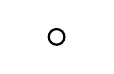
\begin{tikzpicture}
[-,thick,%
  nodeDecorate/.style={shape=circle,inner sep=2pt,draw,thick},%
  scale=0.5]
%% nodes or vertices
\node at (0,0) [nodeDecorate] {};
%% stub nodes that should not be visible
\node at (-0.5,0) {};
\node at (0.5,0) {};
\end{tikzpicture}
}
%%
%%
\qquad
\subfigure[$\cF_1$]{
\begin{tikzpicture}
[-,thick,%
  every node/.style={shape=circle,inner sep=2pt},%
  scale=0.5]
\node[draw,thick] {}
  [sibling distance=1cm]
  child {node[draw,thick] {}}
  child {node[draw,thick] {}};
%% stub nodes that should not be visible
\node at (-0.6,0) {};
\node at (0.6,0) {};
\end{tikzpicture}
}
%%
%%
\qquad
\subfigure[$\cF_2$]{
\begin{tikzpicture}
[-,thick,%
  every node/.style={shape=circle,inner sep=2pt,draw,thick},%
  scale=0.5]
\node {}
  child {node {}}
  child {node {}
    [sibling distance=1cm]
    child {node {}}
    child {node {}}
  };
\end{tikzpicture}
}
%%
%%
\qquad
\subfigure[$\cF_3$]{
\begin{tikzpicture}
[-,thick,%
  every node/.style={shape=circle,inner sep=2pt,draw,thick},%
  scale=0.5]
\node {}
  [sibling distance=2cm]
  child {node {}
    [sibling distance=1cm]
    child {node {}}
    child {node {}}
  }
  child {node {}
    [sibling distance=1cm]
    child {node {}}
    child {node {}
      child {node {}}
      child {node {}}
    }
  };
\end{tikzpicture}
}
%%
%%
\qquad
\subfigure[$\cF_4$]{
\begin{tikzpicture}
[-,thick,%
  every node/.style={shape=circle,inner sep=2pt,draw,thick},%
  scale=0.5]
\node {}
  [sibling distance=4cm]
  child {node {}
    [sibling distance=1cm]
    child {node {}}
    child {node {}
      child {node {}}
      child {node {}}
    }
  }
  child {node {}
    [sibling distance=2cm]
    child {node {}
      [sibling distance=1cm]
      child {node {}}
      child {node {}}
    }
    child {node {}
      [sibling distance=1cm]
      child {node {}}
      child {node {}
        child {node {}}
        child {node {}}
      }
    }
  };
\end{tikzpicture}
}
%%
%%
\qquad
\subfigure[$\cF_5$]{
\begin{tikzpicture}
[-,thick,%
  every node/.style={shape=circle,inner sep=2pt,draw,thick},%
  scale=0.5]
\node {}
  [sibling distance=6cm]
  child {node {}
    [sibling distance=2cm]
    child {node {}
      [sibling distance=1cm]
      child {node {}}
      child {node {}}
    }
    child {node {}
      [sibling distance=1cm]
      child {node {}}
      child {node {}
        child {node {}}
        child {node {}}
      }
    }
  }
  child {node {}
    [sibling distance=4cm]
    child {node {}
      [sibling distance=1cm]
      child {node {}}
      child {node {}
        child {node {}}
        child {node {}}
      }
    }
    child {node {}
      [sibling distance=2cm]
      child {node {}
        [sibling distance=1cm]
        child {node {}}
        child {node {}}
      }
      child {node {}
        [sibling distance=1cm]
        child {node {}}
        child {node {}
          child {node {}}
          child {node {}}
        }
      }
    }
  };
\end{tikzpicture}
}
\end{figure}

\end{document}

\caption{Fibonacci trees of heights $n = 0, 1, 2, 3, 4, 5$.}
\label{fig:tree_data_structures:Fibonacci_trees_1_to_5}
\end{figure}

\begin{figure}[!htbp]
\centering
\index{Fibonacci!tree}
%%%%%%%%%%%%%%%%%%%%%%%%%%%%%%%%%%%%%%%%%%%%%%%%%%%%%%%%%%%%%%%%%%%%%%%%%%%
%% This file is part of the book
%%
%% Algorithmic Graph Theory
%% http://code.google.com/p/graph-theory-algorithms-book/
%%
%% Copyright (C) 2009, 2010, 2011 Minh Van Nguyen <nguyenminh2@gmail.com>
%%
%% See the file COPYING for copying conditions.
%%%%%%%%%%%%%%%%%%%%%%%%%%%%%%%%%%%%%%%%%%%%%%%%%%%%%%%%%%%%%%%%%%%%%%%%%%%

\documentclass{article}

\usepackage{tikz}
\usetikzlibrary{external}
\usetikzlibrary{trees}
\tikzexternalize{Fibonacci-tree-height}

\begin{document}

\begin{figure}
\begin{tikzpicture}
[-,thick,%
  every node/.style={shape=circle,inner sep=1.5pt,draw,thick},%
  scale=0.7]
\scriptsize
\node {$6$}
  [sibling distance=10cm]
  child {node {$4$}
    [sibling distance=4cm]
    child {node {$2$}
      [sibling distance=1cm]
      child {node {$0$}}
      child {node {$1$}
        child {node {$0$}}
        child {node {$0$}}
      }
    }
    child {node {$3$}
      [sibling distance=2cm]
      child {node {$1$}
        [sibling distance=1cm]
        child {node {$0$}}
        child {node {$0$}}
      }
      child {node {$2$}
        [sibling distance=1cm]
        child {node {$0$}}
        child {node {$1$}
          child {node {$0$}}
          child {node {$0$}}
        }
      }
    }
  }
  child {node {$5$}
    [sibling distance=6cm]
    child {node {$3$}
      [sibling distance=2cm]
      child {node {$1$}
        [sibling distance=1cm]
        child {node {$0$}}
        child {node {$0$}}
      }
      child {node {$2$}
        [sibling distance=1cm]
        child {node {$0$}}
        child {node {$1$}
          child {node {$0$}}
          child {node {$0$}}
        }
      }
    }
    child {node {$4$}
      [sibling distance=4cm]
      child {node {$2$}
        [sibling distance=1cm]
        child {node {$0$}}
        child {node {$1$}
          child {node {$0$}}
          child {node {$0$}}
        }
      }
      child {node {$3$}
        [sibling distance=2cm]
        child {node {$1$}
          [sibling distance=1cm]
          child {node {$0$}}
          child {node {$0$}}
        }
        child {node {$2$}
          [sibling distance=1cm]
          child {node {$0$}}
          child {node {$1$}
            child {node {$0$}}
            child {node {$0$}}
          }
        }
      }
    }
  };
\end{tikzpicture}
\end{figure}

\end{document}

\caption{Fibonacci tree $\cF_6$ with subtree heights for vertex labels.}
\label{fig:tree_data_structures:Fibonacci_tree_F6_subtree_heights}
\end{figure}

\begin{theorem}
\label{thm:tree_data_structures:AVL_tree_logarithmic_height}
\textbf{Logarithmic height.}
The height $h$ of an AVL tree with $n$ internal vertices is bounded by
\[
\lg(n + 1) \leq h < 2 \cdot \lg n + 1.
\]
\end{theorem}

\begin{proof}
Any binary tree of height $h$ has at most $2^i$ leaves. From the proof
of Corollary~\ref{cor:tree_data_structures:height_binary_heap}, we see
that $n$ is bounded by $2^{h - 1} \leq n \leq 2^h - 1$ and in
particular $n + 1 \leq 2^h$. Take the logarithm of both sides to get
$h \geq \lg(n + 1)$.

Now instead of deriving an upper bound for $h$, we find the minimum
order of an AVL tree and from there derive the required upper bound
for $h$. Let $T$ be an AVL tree of minimum order. One subtree of $T$
has height $h - 1$. The other subtree has height $h - 1$ or
$h - 2$. Our objective is to construct $T$ to have as small a number
of vertices as possible. Without loss of generality, let the left and
right subtrees of $T$ have heights $h - 2$ and $h - 1$,
respectively. The Fibonacci tree $\cF_h$ of height $h$ fits the above
requirements for $T$. If $N(h)$ denote the number of internal vertices
of $\cF_h$, then $N(h) = 1 + N(h - 1) + N(h - 2)$ is strictly
increasing so
%%
\begin{equation}
\label{eqn:tree_data_structures:lower_bound_on_minimum_n_nodes}
N(h)
>
N(h - 2) + N(h - 2)
=
2 \cdot N(h - 2).
\end{equation}
%%
Repeated application
of~\eqref{eqn:tree_data_structures:lower_bound_on_minimum_n_nodes}
shows that
%%
\begin{equation}
\label{eqn:tree_data_structures:lower_bound_on_minimum_n_nodes_general}
N(h)
>
2^i \cdot N(h - 2i)
\end{equation}
%%
for any integer $i$ such that $h - 2i \geq 1$. Choose $i$ so that
$h - 2i = 1$ or $h - 2i = 2$, say the former. Substitute
$i = (h - 1) / 2$
into~\eqref{eqn:tree_data_structures:lower_bound_on_minimum_n_nodes_general}
yields $N(h) > 2^{(h - 1) / 2}$. That is, $n > 2^{(h - 1) / 2}$ and
taking logarithm of both sides yields $h < 2 \cdot \lg n + 1$.
\end{proof}

An immediate consequence of
Theorem~\ref{thm:tree_data_structures:AVL_tree_logarithmic_height} is
that any binary\index{binary search tree} search tree implemented as
an AVL tree should have at most logarithmic height. Contrast this with
a general BST of order $N_1$, whose height can be as low as
logarithmic in $N_1$ or as high as linear in $N_1$. Translating to
search time, we see that searching a general BST using
Algorithm~\ref{alg:tree_data_structures:binary_search_tree_locate} is
in the worst case $O(N_1)$, which is no better than searching a sorted
list. However, if $N_2$ is the order of an AVL tree endowed with the
binary\index{binary search tree!property} search tree property, then
searching the AVL tree using
Algorithm~\ref{alg:tree_data_structures:binary_search_tree_locate} has
worst-case $O(\lg N_2)$ runtime. While the worst-case runtime of a
general BST can vary between $O(\lg N_1)$ and $O(N_1)$, that of an AVL
tree with the binary search tree property is at most $O(\lg N_2)$.


%%%%%%%%%%%%%%%%%%%%%%%%%%%%%%%%%%%%%%%%%%%%%%%%%%%%%%%%%%%%%%%%%%%%%%%%%%%

\section{Problems}

\begin{quote}
\footnotesize
No problem is so formidable that you can't walk away from it. \\
\noindent
--- Charles M. Schulz\index{Schulz, Charles M.}
\end{quote}

\begin{problem}
\item Let $Q$ be a priority queue of $n > 1$ elements, given in
  sequence representation. From
  section~\ref{subsec:tree_data_structures:sequence_implementation},
  we know that inserting an element into $Q$ takes $O(n)$ time and
  deleting an element from $Q$ takes $O(1)$ time.
  %%
  \begin{enumerate}[(a)]
  \item Suppose $Q$ is an empty priority queue and let
    $e_0, e_1, \dots, e_n$ be $n + 1$ elements we want to insert into
    $Q$. What is the total runtime required to insert all the $e_i$
    into $Q$ while also ensuring that the resulting queue is a
    priority queue?

  \item Let $Q = [e_0, e_1, \dots, e_n]$ be a priority queue of
    $n + 1$ elements. What is the total time required to remove all
    the elements of $Q$?
  \end{enumerate}

\item Prove the correctness of
  Algorithms~\ref{alg:tree_data_structures:binary_heap_insert}
  and~\ref{alg:tree_data_structures:binary_heap_delete}.

\item Describe a variant of
  Algorithm~\ref{alg:tree_data_structures:binary_heap_delete} for
  modifying the key of the root of a binary heap, without extracting
  any vertex from the heap.

\item Section~\ref{subsec:tree_data_structures:insertion_sift_up}
  describes how to insert an element into a binary heap $T$. The
  general strategy is to choose the first leaf following the last
  internal vertex of $T$, replace that leaf with the new element so
  that it becomes an internal vertex, and perform a sift-up operation
  from there. If instead we choose any leaf of $T$ and replace that
  leaf with the new element, explain why we cannot do any better than
  Algorithm~\ref{alg:tree_data_structures:binary_heap_insert}.

\item Section~\ref{subsec:tree_data_structures:deletion_sift_down}
  shows how to extract the minimum vertex from a binary heap
  $T$. Instead of replacing the root with the last internal vertex of
  $T$, we could replace the root with any other vertex of $T$ that is
  not a leaf and then proceed to maintain the heap-structure and
  heap-order properties. Explain why the latter strategy is not better
  than Algorithm~\ref{alg:tree_data_structures:binary_heap_delete}.

\item Let $S$ be a sequence of $n > 1$ real numbers. How can we use
  algorithms described in
  section~\ref{sec:tree_data_structures:binary_heaps} to sort $S$?

\item The binary heaps discussed in
  section~\ref{sec:tree_data_structures:binary_heaps} are properly
  called minimum\index{binary heap!minimum} binary heaps because the
  root of the heap is always the minimum vertex. A corresponding
  notion is that of maximum\index{binary heap!maximum} binary heaps,
  where the root is always the maximum element. Describe algorithms
  analogous to those in
  section~\ref{sec:tree_data_structures:binary_heaps} for managing
  maximum binary heaps.

\item What is the total time required to extract all elements from a
  binary heap?

\item Numbers of the form $\binom{n}{r}$ are called
  binomial\index{binomial coefficient} coefficients. They also count
  the number of $r$-combinations from a set of $n$ objects.
  Algorithm~\ref{alg:tree_data_structures:generate_all_r_combinations}
  presents pseudocode to generate all the $r$-combinations of a set of
  $n$ distinct objects.
  %%
  \begin{enumerate}[(a)]
  \item What is the worst-case runtime of
    Algorithm~\ref{alg:tree_data_structures:generate_all_r_combinations}?

  \item Prove the correctness of
    Algorithm~\ref{alg:tree_data_structures:generate_all_r_combinations}.
  \end{enumerate}

\item In contrast to enumerating all the $r$-combinations of a set of
  $n$ objects, we may only want to generate a random
  $r$-combination. Describe and present pseudocode of a procedure to
  generate a random $r$-combination of $\{1, 2, \dots, n\}$.

\item A problem related to the $r$-combinations of the set
  $S = \{1, 2, \dots, n\}$ is that of generating the permutations of
  $S$. Algorithm~\ref{alg:tree_data_structures:generate_all_permutations}
  presents pseudocode to generate all the permutations of $S$ in
  increasing lexicographic order. Find the worst-case runtime of this
  algorithm and prove its correctness.

\item Provide a description and pseudocode of an algorithm to generate
  a random permutation of $\{1, 2, \dots, n\}$.

\item Takaoka\index{Takaoka, Tadao}~\cite{Takaoka1999b} presents a
  general method for combinatorial\index{combinatorial generation}
  generation that runs in $O(1)$ time. How can Takaoka's method be
  applied to generating combinations and permutations?

\item The proof of
  Lemma~\ref{lem:tree_data_structures:basic_properties_binomial_trees}
  relies on Pascal's\index{Pascal!formula} formula, which states that
  for any positive integers $n$ and $r$ such that $r \leq n$, the
  following identity holds:
  \[
  \binom{n+1}{r}
  =
  \binom{n}{r-1} + \binom{n}{r}.
  \]
  Prove Pascal's formula.

\item Let $m,n,r$ be nonnegative integers such that $r \leq n$. Prove
  the Vandermonde\index{Vandermonde!convolution} convolution
  \[
  \binom{m + n}{r}
  =
  \sum_{k=0}^r \binom{m}{k} \binom{n}{r-k}.
  \]
  The latter equation, also known as Vandermonde's identity, was
  already known as early as 1303 in China by Chu\index{Chu Shi-Chieh}
  Shi-Chieh. Alexandre-Th\'eophile
  Vandermonde\index{Vandermonde!Alexandre-Th\'eophile} independently
  discovered it and his result was published in 1772.

\begin{algorithm}[!htbp]
%%%%%%%%%%%%%%%%%%%%%%%%%%%%%%%%%%%%%%%%%%%%%%%%%%%%%%%%%%%%%%%%%%%%%%%%%%%
%% This file is part of the book
%%
%% Algorithmic Graph Theory
%% http://code.google.com/p/graph-theory-algorithms-book/
%%
%% Copyright (C) 2009--2011 Minh Van Nguyen <nguyenminh2@gmail.com>
%%
%% See the file COPYING for copying conditions.
%%%%%%%%%%%%%%%%%%%%%%%%%%%%%%%%%%%%%%%%%%%%%%%%%%%%%%%%%%%%%%%%%%%%%%%%%%%

\DontPrintSemicolon
\SetAlgoNoLine
%%
%% data section
\SetKwData{MyMax}{max}
%%
%% input
\KwIn{Two nonnegative integers $n$ and $r$.}
%%
%% output
\KwOut{A list $L$ containing all the $r$-combinations of the set
  $\{1, 2, \dots, n\}$ in increasing lexicographic order.}
\BlankLine
%%
%% algorithm body
$L \assign [\,]$\;
$c_i \assign i$ for $i = 1, 2, \dots, r$\;
$\append(L,\, c_1 c_2 \cdots c_r)$\;
\For{$i \assign 2, 3, \dots, \binom{n}{r}$}{
  $m \assign r$\;
  $\MyMax \assign n$\;
  \While{$c_m = \MyMax$}{
    $m \assign m - 1$\;
    $\MyMax \assign \MyMax - 1$\;
  }
  $c_m \assign c_m + 1$\;
  $c_j \assign c_{j-1} + 1$ for $j = m + 1, m + 2, \dots, r$\;
  $\append(L,\, c_1 c_2 \cdots c_r)$\;
}
\Return $L$\;

\caption{Generating all the $r$-combinations of $\{1, 2, \dots, n\}$.}
\label{alg:tree_data_structures:generate_all_r_combinations}
\end{algorithm}

\begin{algorithm}[!htbp]
%%%%%%%%%%%%%%%%%%%%%%%%%%%%%%%%%%%%%%%%%%%%%%%%%%%%%%%%%%%%%%%%%%%%%%%%%%%
%% This file is part of the book
%%
%% Algorithmic Graph Theory
%% http://code.google.com/p/graph-theory-algorithms-book/
%%
%% Copyright (C) 2009--2011 Minh Van Nguyen <nguyenminh2@gmail.com>
%%
%% See the file COPYING for copying conditions.
%%%%%%%%%%%%%%%%%%%%%%%%%%%%%%%%%%%%%%%%%%%%%%%%%%%%%%%%%%%%%%%%%%%%%%%%%%%

\DontPrintSemicolon
\SetAlgoNoLine
%%
%% input
\KwIn{A positive integer $n$.}
%%
%% output
\KwOut{A list $L$ containing all the permutations of
  $\{1, 2, \dots, n\}$ in increasing lexicographic order.}
\BlankLine
%%
%% algorithm body
$L \assign [\,]$\;
$c_i \assign i$ for $i = 1, 2, \dots, n$\;
$\append(L,\, c_1 c_2 \cdots c_n)$\;
\For{$i \assign 2, 3, \dots, n!$}{
  $m \assign n - 1$\;
  \While{$c_m > c_{m+1}$}{
    $m \assign m - 1$\;
  }
  $k \assign n$\;
  \While{$c_m > c_k$}{
    $k \assign k - 1$\;
  }
  swap the values of $c_m$ and $c_k$\;
  $p \assign m + 1$\;
  $q \assign n$\;
  \While{$p < q$}{
    swap the values of $c_p$ and $c_q$\;
    $p \assign p + 1$\;
    $q \assign q - 1$\;
  }
  $\append(L,\, c_1 c_2 \cdots c_n)$\;
}
\Return $L$\;

\caption{Generating all the permutations of $\{1, 2, \dots, n\}$.}
\label{alg:tree_data_structures:generate_all_permutations}
\end{algorithm}

\item If $m$ and $n$ are nonnegative integers, prove that
  \[
  \binom{m + n + 1}{n}
  =
  \sum_{k=0}^n \binom{m + k}{k}.
  \]

\item Let $n$ be a positive integer. How many distinct
  binomial\index{binomial heap} heaps having $n$ vertices are there?

\item The algorithms described in
  section~\ref{sec:tree_data_structures:binomial_heaps} are formally
  for minimum\index{binomial heap!minimum} binomial heaps because the
  vertex at the top of the heap is always the minimum vertex. Describe
  analogous algorithms for maximum\index{binomial heap!maximum}
  binomial heaps.

\item If $H$ is a binomial\index{binomial heap} heap, what is the
  total time required to extract all elements from $H$?

\item Frederickson\index{Frederickson, Greg N.}~\cite{Frederickson1993}
  describes an $O(k)$ time algorithm for finding the $k$-th smallest
  element in a binary heap. Provide a description and pseudocode of
  Frederickson's algorithm and prove its correctness.

\item Fibonacci heaps~\cite{FredmanTarjan1984} allow for amortized
  $O(1)$ time with respect to finding the minimum element,
  inserting an element, and merging two Fibonacci heaps. Deleting the
  minimum element takes amortized time $O(\lg n)$, where $n$ is the
  number of vertices in the heap. Describe and provide pseudocode of
  the above Fibonacci heap operations and prove the correctness of the
  procedures.

\item Takaoka\index{Takaoka, Tadao}~\cite{Takaoka1999a} introduces
  another type of heap called a $2$-$3$ heap. Deleting the minimum
  element takes amortized $O(\lg n)$ time with $n$ being the number of
  vertices in the $2$-$3$ heap. Inserting an element into the heap
  takes amortized $O(1)$ time. Describe and provide pseudocode of the
  above $2$-$3$ heap operations. Under which conditions would $2$-$3$
  heaps be more efficient than Fibonacci heaps?

\item In 2000, Chazelle\index{Chazelle, Bernard}~\cite{Chazelle2000a}
  introduced the soft heap, which can perform common heap operations
  in amortized $O(1)$ time. He then applied~\cite{Chazelle2000b} the
  soft heap to realize a very efficient implementation of an algorithm
  for finding minimum spanning trees. In 2009,
  Kaplan\index{Kaplan, Haim} and
  Zwick\index{Zwick, Uri}~\cite{KaplanZwick2009} provided a simple
  implementation and analysis of Chazelle's soft heap.
  %%
  \begin{enumerate}[(a)]
  \item Describe soft heaps and provide pseudocode of common heap
    operations.

  \item Prove the correctness of the algorithms and provide runtime
    analyses.

  \item Describe how to use soft heap to realize an efficient
    implementation of an algorithm to produce minimum spanning trees.
  \end{enumerate}

\item Explain any differences between the binary
  heap-order\index{binary heap!order property} property, the
  binomial heap-order\index{binomial heap!order property}
  property, and the binary
  search\index{binary search tree!property} tree property. Can
  in-order traversal be used to list the vertices of a binary heap in
  sorted order? Explain why or why not.

\item Present pseudocode of an algorithm to find a vertex with maximum
  key in a binary search tree.

\item Compare and contrast algorithms for locating minimum and maximum
  elements in a list with their counterparts for a binary search tree.

\item Let $T$ be a nonempty BST and suppose $v \in V(T)$ is not a
  minimum vertex of $T$. If $h$ is the height of $T$, describe and
  present pseudocode of an algorithm to find the predecessor of $v$ in
  worst-case time $O(h)$.

\item Let $L = [v_0, v_1, \dots, v_n]$ be the in-order listing of a
  BST $T$. Present an algorithm to find the successor of
  $v \in V(T)$ in constant time $O(1)$. How can we find the
  predecessor of $v$ in constant time as well?

\item Modify
  Algorithm~\ref{alg:tree_data_structures:binary_search_tree_delete}
  to extract a minimum vertex of a binary search tree. Now do the same
  to extract a maximum vertex. How can
  Algorithm~\ref{alg:tree_data_structures:binary_search_tree_delete}
  be modified to extract a vertex from a binary search tree?

\item Let $v$ be a vertex of a BST and suppose $v$ has two
  children. If $s$ and $p$ are the successor and predecessor of $v$,
  respectively, show that $s$ has no left-child and $p$ has no
  right-child.

\item Let $L = [e_0, e_1, \dots, e_n]$ be a list of $n + 1$ elements
  from a totally ordered set $X$ with total order $\leq$. How can
  binary search trees be used to sort $L$?

\item Describe and present pseudocode of a recursive algorithm for
  each of the following operations on a BST.
  %%
  \begin{enumerate}[(a)]
  \item Find a vertex with a given key.

  \item Locate a minimum vertex.

  \item Locate a maximum vertex.

  \item Insert a vertex.
  \end{enumerate}

\item Are the algorithms presented in
  section~\ref{sec:tree_data_structures:binary_search_trees} able to
  handle a BST having duplicate keys? If not, modify the relevant
  algorithm(s) to account for the case where two vertices in a BST
  have the same key.

\item The notion of vertex level for binary trees can be extended to
  general rooted trees as follows. Let $T$ be a rooted tree with
  $n > 0$ vertices and height $h$. Then level\index{level!tree}
  $0 \leq i \leq h$ of $T$ consists of all those vertices in $T$ that
  have the same depth $i$. If each vertex at level $i$ has $i + m$
  children for some fixed integer $m > 0$, what is the number of
  vertices at each level of $T$?
\end{problem}
